% !TeX spellcheck = en_US
\RequirePackage{ifluatex, ifxetex} % these are for the portability of this example - can be omitted in any actual document made for a certain engine

\ifnum 0\ifxetex 1\fi\ifluatex 1\fi>0
\else
  % only needed for using Greek letters outside math when running PDFLaTeX - leave out otherwise
  %\PassOptionsToPackage{LGR}{fontenc}
  %\RequirePackage{textgreek}
\fi

% Own environment definitions.
\newenvironment{it} {\itshape}


\documentclass[globalnumbering,centeredcaptions,draftfooter]{tutthesis} % see appendix for list of options

%\pagestyle{headings} % Adds titles to the header


% ifnameyear is defined to demonstrate both versions in a single file. You may leave it out and simply use one version throughout your file.
\newif\ifnameyear
\nameyearfalse



% ==============
% Basic packages
% ==============
% You should use these unless you really know what you're doing

\ifnum 0\ifxetex 1\fi\ifluatex 1\fi>0
\else\usepackage[utf8]{inputenc}
\fi

\usepackage[english,finnish]{babel} % The language of the thesis last

% If you are working with a minimal LateX distribution, you may have to install some extra packages. Make sure that at least babel-finnish (available in e.g. texlive-lang-european) and the basic fonts (e.g. texlive-fonts-recommended) are installed.

\usepackage{babelbib} % You should use this unless you are using biblatex. Add option fixlanguage if you're writing in English (the thesis writing guide is asymmetric, requiring Finnish theses to have e.g. 'eds.' for sources in English, while requiring English theses to have all such parts in English)

\ifnameyear\usepackage{natbib} % add option longnamesfirst if you want to have full author list with first citation
\else\providecommand{\citep}{\cite} % This template is written using \citep to get name-year citations right, and in numerical mode the command is here aliased to the standard \cite. If you use numbered citations, leave this out and use \cite
\fi


% ===============
% Useful packages
% ===============
% Packages which are not required for a thesis that follows guidelines, but may be convenient or necessary in common cases

%\usepackage{microtype} % subtle but nice improvements to how text is printed

%\usepackage{textcase} % may be used to keep parts of title lowercase

\usepackage{array}
\usepackage{tabularx} % e.g. multiline cells
%\usepackage{calc} %for performing length arithmetic such as column width = text width minus some other width
%\usepackage{longtable} % for tables spanning multiple pages

%\usepackage{psfrag} % editing ps files
%\usepackage{subfig} % parallel small figures a,b,c,...
%\usepackage{rotating} % for rotating e.g. full-page figures

%\usepackage{siunitx} % nice formatting for combinations of number and unit
\usepackage{amsopn} % For operator names; not necessary if amsmath is used
%\usepackage[fleqn]{amsmath} %Extensions to math handling; if you use this, you should use e.g. gather instead of equation due to a hyperref bug

\usepackage{listings} %Typesetting code
%\lstset{basicstyle=\footnotesize\ttfamily, numbers=left}
%\renewcommand{\lstlistingname}{Ohjelma} % Program if you're writing in English
% If you want non-ASCII characters (e.g. in comments), check out the listingsutf8 package

\ifnum 0\ifxetex 1\fi\ifluatex 1\fi>0
  \usepackage[math-style=ISO]{unicode-math} %must not precede amsmath and most other math and font related packages
\else
  %\usepackage{bm} % The \bm command is used for bold italic variables used in some fields not to be used with unicode-math
  %\usepackage[helvratio=1]{newtxtext} \usepackage{newtxmath}% some recommend the newtx fonts
  \usepackage{textcomp} % symbols like \textdegree
\fi


% ===========================
% Bibliographic information
% ===========================
% These must be set before loading pdfx or beginning document
\author{Mauri Mustonen}
\title{sähköaseman älykkään elektroniikkalaitteen viestien tilaus ja prosessointi}
\datesubmitted{2018}{5}{17} % year, month, day; no leading zeroes; submitted for bachelor's theses and thesisapproved for master’s
\thesistype{Diplomityö} % Do not use ASCII apostrophe ' as it will not be substituted with the correct one (’) in the PDF metadata. Note that there are both short version (this) and a long one - "Master’s" vs. "Master of Science"
\major{Ohjelmistotuotanto}
\programme{Tietotekniikan koulutusohjelma} % Note apostrophes on all fields for PDF metadata
\examiner{Professori Kari Systä} %\and for plural
%\datetopicapproved{2017}{1}{5} % only for master’s theses
\keywords{Ohjelmistotuotanto, IEC 61850, MMS, AMQP}


% Packages that need to be loaded late
% ----------------------------------------------
% \usepackage[a-2u]{pdfx} % If you're using PDFLatex and your version of pdfx is not recent enough, you may run into the inputencoding bug. In that case, load inputenc after pdfx (and replace any non-ASCII characters in the metadata with e.g. \"{a})

\usepackage{hyperref} % This must (usually) be the last package you load - load this OR pdfx (which also loads hyperref). Usage of pdfx would be nice, but if you have issues with that you may fall back to just hyperref



\begin{document}


\maketitle
%First, the abstract in the language of the thesis (no language selection). Note that most fields are already defined.
\thesisdescription{Diplomityö}


\begin{abstract}
\begin{it}
	Kirjoita yleiskataus tiivistelmä työstä tähän. Kerro lyhyesti mitä työssä tullaan tekemään.
\end{it}
\end{abstract}


%Then, the abstract in the other language (explicit language selection) except for bachelor's theses
\iffalse
\begin{otherlanguage}{english}

\title{Tampere University of Technology thesis template}
\programme{...}
\thesisdescription{...}
\major{Mathematics}
\examiner{Professor Vilma Välkky\and Professor Matti Meikäläinen}
\keywords{thesis, template, thesis structure, thesis layout}

\begin{abstract}
The abstract is a self-contained, concise description of the thesis: what was the problem, what was done, what was the result.
Do not include charts or tables in the abstract.

First include the abstract written in the main language of the thesis and then the translation.
A bachelor's thesis in Finnish must also have a name in English for archival.
\end{abstract}
\end{otherlanguage}
\fi


\chapter*{Alkusanat}
\label{ch:alkusanat}

\begin{it}
	Mistä tämän diplomityönaiheen sain ja kiittää eri ihmisiä ketä työssä oli sidoshenkilöinä.
\end{it}

\vspace{2\baselineskip}

Tampereella, 19.4.2018

\vspace{2\baselineskip}

Mauri Mustonen


% Create table of content.
\tableofcontents


% List of figures and tables.
% \listoffigures
% \listoftables


\chapter*{Lyhenteet ja merkinnät}
\label{ch:lyhenteetjamerkinnat}

% This is not a "proper" table, so no table environment
% Suppressed left colsep; 20% - 1 x colsep; right colpsep; left colpadding; 80% - 1 x colpadding; suppressed right colpadding
\begin{tabular}[h]{@{} p{0.2\textwidth-\tabcolsep} p{0.8\textwidth-\tabcolsep} @{}}
	AMQP & engl. \emph{Advanced Message Queuing Protocol} \\
	FFI & engl. \emph{Foreign Function Interface}, mekanismi, jolla ajettava ohjelma voi kutsua toisella kielellä implementoitua funktiota\\
	GIL & engl. \emph{Global Interpreter Lock}, tulkattavassa kielissä oleva globaali lukitus, joka rajoittaa yhden säikeen suoritukseen kerrallaan \\
	HAL & engl. \emph{Hardware Abstraction Layer}, laitteistoabstraktiotaso abstraktoimaan laitteen toiminnalisuus lähdekoodista \\
	IED & engl. \emph{Intelligent Electronic Device}, konfiguroitava sähköaseman älykäs elektroninen laite, joka toteuttaa aseman toiminnallisuutta \\
	MMS & engl. \emph{Manufacturing Message Specification} \\
	RCB & engl. \emph{Report Control Block}, raporttien konfigurointiin ja tilaukseen tarkoitettu lohko asiakasohjelmalle \\
\end{tabular}


% Each chapter is it's own file and included here.
\chapter{Johdanto}
\label{ch:johdanto}
\begin{it}
	Kirjoita tähän johdantoa työstä ja aiheesta. Kuinka työ valittiin ja miksi tekijä valitsi tämän työn. Kirjoita myös mitä tehtiin. Kokonaiskuva työstä pitäisi saada johdannosta. Alusta lukijaa todella hyvin yleismaallisella kuvalla ja taustalla. Asiaa pitäisi olla hyvin hallussa ennen teoriaosuuteen siirtymistä.
\end{it}

\section{Tausta}

\section{Laajuus}

\section{Tavoitteet}
\chapter{Teoria}
\label{ch:teoria}
Tässä osiossa lukijaa perehdytetään työn kannalta tärkeään teoriaan. Teoriaosuuden kokonaan lukemalla lukija ymmärtää, mitä IEC 61850 -standardi tarkoittaa sähköasemien kannalta ja mihin sitä käytetään. Lisäksi kuinka standardi määrittää viestien tilauksen mekanismit ulkopuoliselle ohjelmalle ja mitä siihen liittyy. Standardi on todella laaja ja tässä osuudessa siitä käsitellään vain tämän työn kannalta oleellinen asia. Tässä työssä toteutettu ohjelmisto julkaisi prosessoidut viestit eteenpäin jonopalvelimelle, mistä muut ohjelmat pystyivät tilaamaan viestejä. Käytetyn jonopalvelin toteutus pohjautui AMQP-standardiin (engl. Advanced Message Queuing Protocol). Teorian viimeisessä osassa perehdytään AMQP-standardiin ja kuinka jonopalvelin sen pohjalta toimii.


\section{IEC 61850 -standardi yhteiseen kommunikointiin}
Sähköasemilla nykypäivänä käytössä olevilla älykkäillä elektronisilla laitteilla (engl. Intelligent Electronic Device, lyhennetään IED) toteutetaan aseman toiminnalisuuden funktioita. Aseman toiminnallisuuteen liittyy sen kontrollointi ja suojaus. Aseman komponenttien suojauksen lisäksi, siihen kuuluu myös asemalta lähtevät sähkölinjat. Hyvä esimerkki sähköaseman suojauksesta on korkeajännitelinjan katkaisija, joka katkaisee virran linjasta vikatilanteissa, kuten linjan poikkimeno kaatuneen puun tai pylvään takia. Fyysistä katkaisijaa ohjaa aseman automatiikka, joka toteutetaan IED-laitteilla. IED-laite voi olla kytketty fyysisesti ohjattavaan laitteeseen \cite[s.~63--64]{IEC61850-7-1}. Koko sähköaseman toiminnallisuus koostuu monesta eri funktiosta, jotka on jaettu monelle IED-laitteelle. Jotta systeemi pystyy toimimaan, täytyy IED-laitteiden kommunikoida keskenään ja vaihtaa informaatiota toistensa kanssa. IED-laitteiden täytyy myös kommunikoida asemalta ulospäin erilliselle ohjausasemalle monitorointia ja etäohjausta varten \cite[s.~1]{Brunner2008}. On selvää, että monimutkaisen systeemin ja monen valmistajien kesken tarvitaan yhteiset säännöt kommunikointia varten.

Maailmanlaajuisesti määritetty IEC 61850 -standardi määrittää sähköaseman sisäisen kommunikoinnin säännöt IED-laitteiden välillä. Standardi määrittää myös säännöt asemalta lähtevään liikenteeseen, kuten toiselle sähköasemalle ja ohjausasemalle \cite[s.~10]{IEC61850-7-1}. Ilman yhteistä standardia, jokainen valmistaja olisi vapaa toteuttamaan omat säännöt ja protokollat kommunikointiin. Seurauksena olisi, että laitteet eivät olisi keskenään yhteensopivia eri valmistajien kesken. Standardin tarkoitus on poistaa yhteensopivuusongelmat ja määrittää yhteiset säännöt kommunikoinnin toteuttamiseen \cite[s.~1]{Kaneda2008}.

Tärkeä ja iso osa standardia on sähköaseman systeemin funktioiden abstrahointi mallien kautta. Standardi määrittää tarkasti kuinka abstraktit mallit määritellään aseman oikeista laiteista ja niiden ominaisuuksista. Tarkoituksena on tehdä mallit tekniikasta ja toteutuksesta riippumattomaksi. Tämän jälkeen määritellään kuinka mallit toteutetaan erikseen toimivaksi jollekin tekniikalle. Abstrahoituja malleja käytetään myös määrittämään sähköaseman IED-laitteiden ja aseman muiden osien konfigurointi. Tekniikasta riippumattomien mallien ansiosta standardi on pohjana tulevaisuuden laajennoksille ja tekniikoille. Uusien tekniikoiden ilmaantuessa, voidaan standardiin lisätä  osa, joka  toteuttaa abstraktimallit kyseiselle tekniikalle \cite[s.~2]{Brunner2008}. Tässä työssä standardin malleja ja palveluita käytettiin MMS-protokollan (engl. Manufacturing Message Specification) toteutuksella. MMS-protokolla on maailmanlaajuinen ISO 9506 -standardi, joka on määritetty toimivaksi TCP/IP:n pinon päällä \cite{MMS-protocol-stack-and-API}. Jokainen verkkoon kytkety IED-laite tarvitsee IP-osoitteen kommunikointiin.


\subsection{Standardin eri osat ja niiden merkitykset}	
IEC 61850 -standardi on laaja kokonaisuus. Tämän takia se on pilkottu erillisiin dokumentteihin, joista jokainen käsittelee omaa asiaansa. Historian saatossa standardiin on lisätty uusia dokumentteja laajentamaan standardia \cite{IEC61850series, New-documents-by-IEC-TC-57} \cite[s.~13]{IEC61850-1}. Tämän työn kirjoitushetkellä standardiin kuului lisäksi paljon muitakin dokumentteja, esimerkiksi uusiin toteutuksiin muille tekniikoille ja vesivoimalaitoksien mallintamiseen liittyviä dokumentteja. Laajuudesta huolimatta standardin voi esittää 10:llä eri pääkohdalla ja näiden alakohdilla. Taulukossa \ref{tab:iec61850-dokumentin-osat} on esitetty standardin pääkohdan dokumentit ja niiden alkuperäiset englanninkieliset otsikot \cite[s.~2]{Mackiewicz2006} \cite{IEC61850series}. Kuvassa \ref{fig:iec61850-osat-ja-relaatiot} on esitetty kaikki standardin eri osat ja niiden väliset relaatiot toisiinsa \cite[s.~14]{IEC61850-7-1} \cite[s.~22]{IEC61850-1}. Kuvaan on merkitty yhteinäisellä viivalla ne osat, jotka ovat tämän työn kannalta tärkeitä, ja katkoviivalla ne, jotka eivät ole. Kuvassa käytetään standardin osien englanninkielisiä otsikoita.

\begin{table}[ht!]
	\caption{IEC 61850 -standardin pääkohtien ja niiden alakohtien dokumentit.}
	\label{tab:iec61850-dokumentin-osat}
	\begin{tabular}{l | l}
		\hline
		\textbf{Osa} & \textbf{Otsikko englanniksi} \\
		\hline \hline
		1 & Introduction and overview \\
		2 & Glossary \\
		3 & General requirements \\
		4 & System and project management \\
		5 & \parbox[t]{13cm}{Communication requirements for functions and device models} \\
		6 & \parbox[t]{13cm}{Configuration description language for communication in power utility \par automation systems related to IEDs} \\
		7-1 & \parbox[t]{13cm}{Basic communication structure - Principles and models} \\
		7-2 & \parbox[t]{13cm}{Basic information and communication structure - Abstract communication service interface (ACSI)} \\
		7-3 & \parbox[t]{13cm}{Basic communication structure - Common data classes} \\
		7-4 & \parbox[t]{13cm}{Basic communication structure - Compatible logical node classes and data object classes} \\
		8-1 & \parbox[t]{13cm}{Specific communication service mapping (SCSM) - \par  Mappings to MMS (ISO 9506-1 and ISO 9506-2) and to ISO/IEC 8802-3} \\
		9-2 & \parbox[t]{13cm}{Specific communication service mapping (SCSM) - \par  Sampled values over ISO/IEC 8802-3} \\
		9-3 & \parbox[t]{13cm}{Precision time protocol profile for power utility automation} \\
		10 & Conformance testing \\
		\hline
	\end{tabular}
\end{table}

\begin{figure}[ht!]
	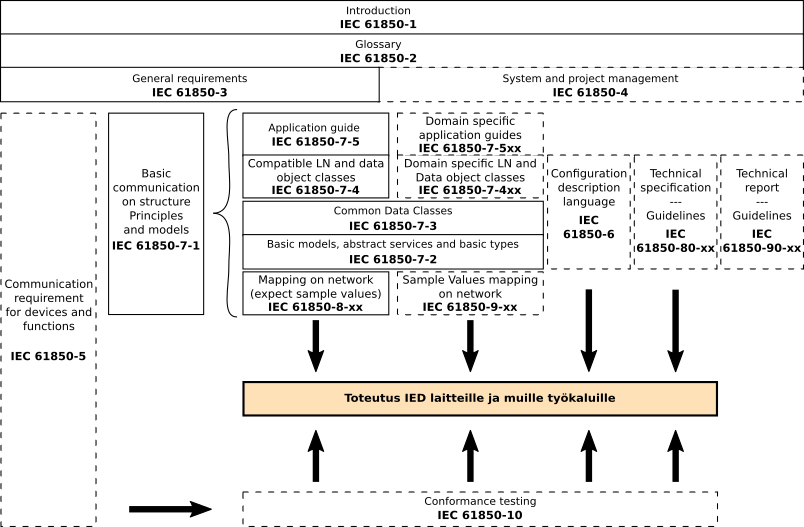
\includegraphics[width=1\textwidth]{pictures/iec61850-series-parts-and-relations.png}
	\caption{IEC 61850 -standardin osat ja niiden väliset relaatiot.}
	\label{fig:iec61850-osat-ja-relaatiot}
\end{figure}

Standardin ensimmäiset osat 1--5 kattavat yleistä kuvaa standardista ja sen vaatimuksista. Osiossa 6 käsitellään IED-laitteiden konfigurointiin käytetty XML (engl. Extensible Markup Language) -pohjainen kieli \cite[s.~7--8]{IEC61850-6}. Tämä osuus ei ole tämän työn kannalta tärkeä ja sitä ei sen tarkemmin käsitellä. Osat 7-1--7-4 käsittelevät standardin abstraktia mallia, niiden palveluita ja kuinka se rakentuu. Abstrahoidut palvelut ja mallit standardissa lyhennetään ACSI (engl. Abstract Communication Service Interface), ja samaa lyhennettä käytetään tässä työssä \cite[s.~72]{IEC61850-7-1}. Osissa 8--9 ja niiden alakohdissa käsitellään abstraktimallien toteuttamista erillisille protokollille, jolloin malleista tulee kyseisestä tekniikasta riippuvaisia. Tässä työssä käytettiin osaa 8-1, joka toteuttaa absrahit mallit MMS-protokollalle. Osa 10 käsittelee testausmenetelmiä, joilla voidaan varmistaa standardin määritysten noudattaminen. Tämä osuus ei myöskään ole tämän työn kannalta tärkeä, ja sitä ei teoriassa sen tarkemmin käsitellä. \cite[s.~15]{IEC61850-7-1}


\subsection{Abstraktimallin käsitteet ja niiden käyttö}
IEC 61850 -standardin lähtökohtana on pilkkoa koko sähköaseman toiminnallisuuden funktiot pieniksi yksilöiksi. Pilkotut yksilöt abstrahoidaan ja pidetään sopivan kokoisina, jotta ne voidaan konfiguroida esitettäväksi erillisellä IED-laiteella. Yksi aseman funktio voidaan hajauttaa monelle eri IED-laitteelle. Esimerkiksi linjan suojaukseen liittyvät komponentit, katkaisija (engl. circuit braker) ja ylivirtasuoja (engl. overcurrent protection). Toimiakseen yhdessä, laitteiden täytyy vaihtaa informaatiota keskenään verkon yli \cite[s.~31]{IEC61850-7-1}. Standardi määrittää seuraavat käsitteet sähköaseman funktioiden mallintamiseen:
\begin{itemize}
	\item fyysinen laite (engl. physical device, lyhennetään PD),
	\item looginen laite (engl. logical device, lyhennetään LD),
	\item looginen noodi (engl. logical node, lyhennetään LN),
	\item dataobjekti (engl. data object, lyhennetään DO),
	\item data-attribuutti (engl. data atribute, lyhennetään DA).
\end{itemize}
Käsiteet muodostavat mallista hiearkisen puurakenteen ja ne on listattu hierarkisessa järjestyksessä. Puun juurena on fyysinen laite, sen alla voi olla yksi tai useampi looginen laite, loogisen laitteen alla yksi tai useampi looginen noodi jne. Käsitteillä standardissa virtualisoidaan aseman funktiot, esimerkiksi suojaus. Kuvassa \ref{fig:substation-abstraction} on esitetty, kuinka sähköaseman fyysiset laitteet voidaan mallintaa standardin määrittämillä käsitteillä. Samaa periaatetta käytetään kaikille aseman laitteille. Kuvassa ensin uloimpana on fyysinen laite, joka ohjaa aseman oikeita laitteita ja tarkkailee niiden toimintaa. Tämä laite voi olla IED-laite, joka on myös samalla kytketty aseman verkkoon ja sillä on IP-osoite. Yksi IED-laite voi olla samaan aikaan kytkettynä aseman moneen muuhun oikeaan laitteeseen. Tämän jälkeen mallinnetaan aseman joukko laitteita loogiseksi laitteeksi. Tällainen voi esimerkiksi olla tietyn jännitetason (engl. bay) komponentit, kuten katkaisijat, muuntajat jne. Kuvassa kaksi muuntajaa on mallinnettu yhdeksi loogiseksi laitteeksi, koska ne kuuluvat samaan jännitetasoon. Looginen laite koostuu loogisista noodeista se mallintaa jotakin aseman ohjattavaa yksittäistä laitetta. Kuvassa kaksi muuntajaa mallinnetaan loogisiksi noodeiksi. Jotta oikeaa fyysistä muuntajaa voidaan kuvata mallilla. Täytyy siitä pystyä esittämään mitattavia tai kuvaavia arvoja, esimerkiksi mitatut jännitteen arvot. Näihin tarkoituksiin käyteään käsitteitä dataobjekti ja data-attribuutti. Looginen noodi koostuu dataobjekteista ja dataobjekti koostuu data-attribuuteista. Data-attribuutti esittää yhtä mitattavaa tai kuvaavaa arvoa laitteesta, esimerkiksi sen hetkinen jännite tai laitteen tila. Dataobjekti on tapa koostaa yhteen kuuluvat data-attribuutit saman käsitteen alle, esimerkiksi mittaukseen tai ohjaukseen liittyvät data-attribuutit. \cite[s.~2]{Camachi2017} \cite[s.~24]{IEC61850-1}

\begin{figure}[ht!]
	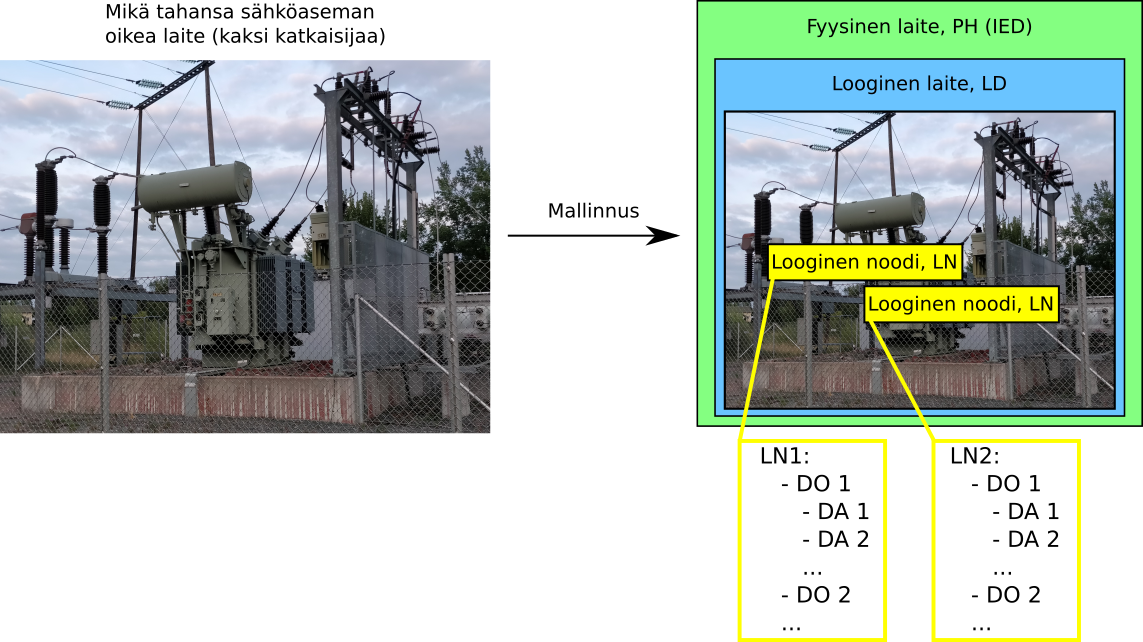
\includegraphics[width=1\textwidth]{pictures/substation-abstraction.png}
	\caption{Sähköaseman fyysisten laiteiden abstrahointi IEC 61850 -standardin käsitteillä (pohjautuu kuvaan \cite[s.~17]{IEC61850-7-1}).}
	\label{fig:substation-abstraction}
\end{figure}

IEC 61850 -standardin käsitteiden avulla sähköaseman laitteet ja funktiot voidaan esittää malleilla. Malleja voidaan käyttää IED-laitteiden konfiguroinnin määrittämiseen ja tietona, jotka voidaan siirtää verkon yli laitteelta toiselle. Jotta käsitteitä voidaan käyttää konfigurointiin ja kommunikointiin, standardi määrittää lisää tarkuutta käsitteisiin ja kuinka niitä käytetään. MMS-protokollan kanssa fyysinen laite yksilöidään IP-osoiteella. Tätä käsitettä ei käytetä kommunikointiin tai konfigurointiin. Fyysisen laitteen käsite on olemassa standardissa, jotta se voidaan pitää abstraktina toteutettavasta tekniikasta. Looginen laite yksilöidään nimellä, joka on yksilöllinen IED-laitteessa. Standardi ei ota kantaa loogisen laitteen nimeämiseen. Looginen noodi yksilöidään IED-laiteella myös nimellä. Looginen noodi esitetään IED-laitteella jonkin standardissa määrittettyjen luokan instanssina. Standardin osassa 7-4 määritetään valmiita luokkia käytettäväksi eri laitteiden esittämiseen. Esimerkiksi katkaija on määritelty luokkaan tyyppiltään XCBR (engl. circuit braker) \cite[s.~105--106]{IEC61850-7-4}. Sähköaseman insinööri, joka konfiguroi IED-laitteen, määrittää konfiguraatiotiedostossa, että kytketty katkaisija esitetään XCBR-luokan instanssina ja nimeää sen standardin ohjeiden mukaan. Näin IED-laite tietää mitä laitetta se esittää ja ohjaa. IED-laitteessa kaikki eri luokkien instanssit yksilöidään nimillä ja niitä käytetään kun olioon viitataan esimerkiksi palvelukutsulla tai konfiguraatiolla. Looginen noodi koostui dataobjekteista. Standardissa dataobjektit on myös määritetty luokkina, joista tehdään instansseja. Erona on, että loogisen noodin luokkan tyyppi määrittää mitä dataobjektin luokkia insansioidaan, ja millä nimellä ne esitettään loogisen noodin instanssissa. Standari määrittää dataobjektien luokkien tyypit standardissa osassa 7-3. Dataobjekti koostuu data-attribuuteista. Kuten loogisen noodin luokan tyyppi, dataobjektin luokka määrittää käytettävät data-attribuutit ja niiden nimet. Tällä kertaa data-attribuutti ei ole välttämättä suoraan ole luokka. Data-attribuutit voivat olla primitiivisiä tyyppejä, kuten integer ja float. Tai ne voivat olla ns. rakennettuja data-attribuutteja (enlg. constructed attribute classes), jotka pitävät sisällään tarkempia data-attribuutteja. Hyvä esimerkki on data attribuutti nimeltään q, jonka tyyppi on Quality. Standardin mukaan tällä tyypillä on vielä aliattribuutteina mm. validity, detailQual jne \cite[s.~11]{IEC61850-7-3}. Standardi ei rajoita sitä, että dataobjektin alla pitää aina data-attribuutteja. Joissakin tapauksissa dataobjektin alla on toinen dataobjekti ja tämän alla vasta data-attribuutit. Kaikkien luokkien tyyppeihin määritetyt kentät ja niiden nimet voi löytyvät standardista. Kappaleessa \ref{ch:luokkien-rakentuminen-instanseista} käydään tarkemmin läpi kuinka luokkien hierarkia standardissa rakentuu. \cite{IEC61850-1, IEC61850-7-1, IEC61850-7-2, IEC61850-7-3}


\subsection{Loogisen noodin luokkien ja attribuuttien rakentuminen}
\label{ch:luokkien-rakentuminen-instanseista}
IEC 61850 -standardissa kaikki luokat määritellään taulukoilla, joissa on standardoitu kentän nimi, tyyppi, selitys ja onko kenttä valinnainen. Tässä teoriaosuudessa mennään syvemmälle luokkien määritykseen. Lisäksi esitetään esimerkkinä kuinka standardin pohjalta instansioitu looginen noodi ja sen alitason dataobjektit ja data-attribuutit rakentuvat. Esimerkissä käytetään kuvan \ref{fig:iec61850-data-modeling} rakennetta. Nimet ja luokkien instanssit konfiguroidaan IED-laitteelle XML-pohjaisella konfiguraatiotiedostolla. Tämä määritellään standardin osassa 6. Kuvassa \ref{fig:iec61850-data-modeling} fyysinen laite on IED-laite ja siihen verkossa viitataan IP-osoitteella 192.192.1.100. IED-laitteelle on konfiguroitu looginen laite nimeltä MyLD. Eri loogiset laitteet IED-laitteella yksilöi vain sen nimi. Loogisella laitteella on kaksi instanssia loogisen noodin luokista nimillä MMXU1 ja XCBR1. MMXU1 instanssi on tyyppiä MMXU (engl. measurement) \cite[s.~57--58]{IEC61850-7-4} ja XCBR1 on tyyppiä XCBR (engl. circuit breaker). Kyseessä on siis vastaavasti mittaukseen liittyvä laite ja aikaisemmin mainittu linjan katkaisija. XCBR1 loogisella noodilla on dataobjekti nimeltään Pos (engl. position), joka on tyyppiä DPC (engl. controllable double point). Ja MMXU1 nimeltään TotW (engl. total active power), joka on tyyppiä MV (engl. measured value). Loogisilla noodeilla on määritetty enemmänkin dataobjekteja eri nimillä, mutta kuvassa \ref{fig:iec61850-data-modeling} on esitetty vai yhdet yksinkertaisuuden takia. Pos dataobjektilla on data-attribuutit nimeltään stVal, q ja t. Ja TotW dataobjektilla on data-attribuutit mag, q ja t. Esimerkin data-attribuutti q on tyyppiä Quality, jolla on alidata-attribuutteja ja attribuutti StVal on tyyppiä boolean.

\begin{figure}[ht!]
	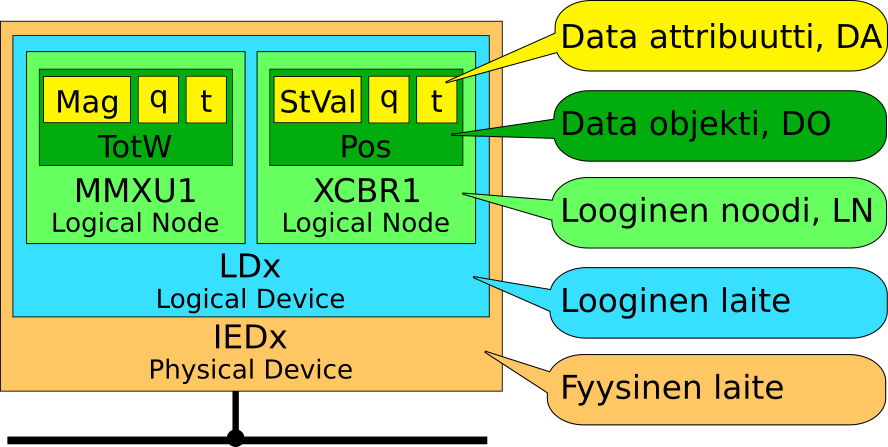
\includegraphics[width=1\textwidth]{pictures/iec61850-data-modeling.png}
	\caption{Standardin käsitteiden hierarkinen rakenne ja niiden nimeämisen esimerkki}
	\label{fig:iec61850-data-modeling}
\end{figure}

Standardissa osassa 7-4 on lista kaikista sen määrittämistä loogisen noodin luokista eri tarkoituksiin. Taulukossa \ref{tab:iec61850-xcbr-class-definition} on esitetty XCBR-luokan määritys. Taulukosta voi nähdä luokan instanssille määritetyt kenttien nimet ja viimeinen sarake M/O/C, kertoo onko kenttä pakollinen (Mandatory, M), valinnainen (Optional, O), vai ehdollinen (Conditional, C) \cite[s.~106]{IEC61850-7-4}. Taulukosta voi nähdä kuvan \ref{fig:iec61850-data-modeling} esimerkin XCBR1-instanssin data-objektin nimeltä Pos ja sen tyypin DPC. Standardissa dataobjektien luokkia kutsutaan yleisiksi luokiksi (engl. Common Data Class, lyhennetään CDC). Näin sen takia, koska samaa dataobjektin luokkaa voidan käyttää monessa eri loogisen noodin luokassa. Standardin dataobjektin luokat on tarkoitettu kerätä yhteen samaan asiaan liittyvät data-attribuutit. CDC-luokkien määritykset löytyvät standardin osasta 7-3 \cite[s.~26]{IEC61850-1}. Joillakin CDC-luokkien attribuutteina voi olla vielä muita CDC-luokkia. Tällöin standardissa puhutaan yleisistä aliluokista (engl. sub data object). Esimerkkinä tästä on CDC-luokka WYE, jolla on attribuuttina phsA niminen kenttä, joka on tyyppiä CMV. CMV on CDC-luokka, jolla on taas omat data attribuuttinsa. \cite[s.~51,61]{IEC61850-7-2} \cite[s.~36]{IEC61850-7-3}

\begin{table}[ht!]
	\caption{IEC 61850 -standardin katkaisijaluokan XCBR -määritys.}
	\label{tab:iec61850-xcbr-class-definition}
	\begin{tabular}{l | l | l | l}
		\hline
		\textbf{Data objektin nimi} & \textbf{Englanniksi} & \textbf{CDC-luokka} & \textbf{M/O/C} \\
		\hline \hline
		\multicolumn{4}{l}{\textbf{Selitys}} \\
		\hline
		EEName & External equipment name plate & DPL & O \\
		\hline
		\multicolumn{4}{l}{\textbf{Tila informaatio}} \\
		\hline
		EEHealt & External equipment health & ENS & O \\
		LocKey & Local or remote key & SPS & O \\
		Loc & Local control behaviour & SPS & M \\
		OpCnt & Operation counter & INS & M \\
		CBOpCap & Circuit breaker operating capability & ENS & O \\
		POWCap & Point on wave switching capability & ENS & O \\
		MaxOpCap & Circuit breaker operating capability & INS & O \\
		Dsc & Discrepancy & SPS & O \\
		\hline
		\multicolumn{4}{l}{\textbf{Mitatut arvot}} \\
		\hline
		SumSwARs & Sum of switched amperes, resettable & BRC & O \\
		\hline
		\multicolumn{4}{l}{\textbf{Kontrollit}} \\
		\hline
		LocSta & Switching authority at station level & SPC & O \\
		Pos & Switch position & DPC & M \\
		BlkOpn & Block opening & SPC & M \\
		BlkCls & Block closing & SPC & M \\
		ChaMotEna & Charger motor enabled & SPC & O \\
		\hline
		\multicolumn{4}{l}{\textbf{Asetukset}} \\
		\hline
		CBTmms & Closing time of braker & ING & O \\
		\hline
	\end{tabular}
\end{table}

Taulukossa \ref{tab:iec61850-DPC-class-definition} on esitetty XCBR-luokan Pos-attribuutin, DPC-luokan määritys \cite[s.~44]{IEC61850-7-3}. Taulukosta voi nähdä kuvan \ref{fig:iec61850-data-modeling} esimerkissä esitetyt data-attribuutit stVal, q ja t ja niiden tyypit. Attribuuttien tyyppejä on paljon enemmänkin ja lukija voi tarvittaessa tarkistaa kaikki tyypit standardista. Tällä periaatteella standardi rakentaa kaikki muutkin luokat hierarkisesti ja sen avulla voidaan selvittää mitä dataobjekteja looginen noodi sisältää, mitä data-attribuutteja kukin data objekti sisältää. Taulukossa \ref{tab:iec61850-DPC-class-definition} on myös määritetty data-attribuuttien funktionaaliset rajoitteet (engl. Functional Constraint, lyhennetään FC), sekä mahdolliset liipaiseimet (engl. trigger options, lyhennetään TrgOp). Nämä kaksi asiaa käsitellään teoriassa myöhemmin.

\begin{table}[ht!]
	\caption{IEC 61850 -standardin DPC-luokan määritys.}
	\label{tab:iec61850-DPC-class-definition}
	\begin{tabular}{l | l | l | l}
		\hline
		\textbf{Data attribuutin nimi} & \textbf{Tyyppi} & \textbf{FC} & \textbf{Liipaisin (TrgOp)} \\
		\hline
		\multicolumn{4}{l}{\textbf{Tila ja ohjaus}} \\
		\hline
		origin & Originator & ST &  \\
		ctlNum & INT8U & ST &  \\
		stVal & CODEC ENUM & ST & dchg \\
		q & Quality & ST & qchg \\
		t & TimeStamp & ST &  \\
		stSeld & BOOLEAN & ST & dchg \\
		opRcvd & BOOLEAN & OR & dchg \\
		opOk & BOOLEAN & OR & dchg \\
		tOpOk & TimeStamp & OR &  \\
		\hline
		\multicolumn{4}{l}{\textbf{Vaihtoehtoinen ja estäminen}} \\
		\hline
		subEna & BOOLEAN & SV &  \\
		subVal & CODED ENUM & SV &  \\
		subQ & Quality & SV &  \\
		subID & VISIBLE STRING64 & SV &  \\
		blkEna & BOOLEAN & BL &  \\
		\hline
		\multicolumn{4}{l}{\textbf{Asetukset, selitys ja laajennos}} \\
		\hline
		pulseConfig & PulseConfig & CF & dchg \\
		ctlModel & CtlModels & CF & dchg \\
		sboTimeOut & INT32U & CF & dchg \\
		sboClass & SboClassses & CF & dchg \\
		operTimeout & INT32U & CF & dchg \\
		d & VISIBLE STRING255 & DC &  \\
		dU & UNICODE STRING255 & DC &  \\
		cdcNs & VISIBLE STRING255 & EX &  \\
		cdcName & VISIBLE STRING255 & EX &  \\
		dataNs & VISIBLE STRING255 & EX &  \\
		\hline
	\end{tabular}
\end{table}

Kaikkien yllämainittujen luokkien kenttien määritysten lisäksi standardi määrittää palveluita jokaiselle luokkatyypille erikseen. Määritetyt palvelut ovat abstrakteja ja ne toteutetaan tekniikalle erillisellä standardin osalla. Palveluita voi ajatella esimerkiksi suoritettavina funktioina. Esimerkkinä palveluista kaikille dataobjekteille on mm. GetDataValues, joka palauttaa kaikki dataobjektin attribuuttien arvot. SetDataValues kirjoittaa annetut data-attribuuttien arvot. Ja GetDataDirectory palauttaa kaikki data-attribuuttien viitteet kyseisessä dataobjekstissa. Näitä ja muita abstrahoituja malleja viitataan standardissa lyhentellä ACSI (engl. abstract communication service interface) \cite[s.~15,45--46]{IEC61850-7-2} \cite[s.~26]{IEC61850-7-1}.


\subsection{Attribuuttien viittaus hierarkiassa}
IEC 61850 -standardi määrittää erilaisia palvelukutsuja eri luokkatyypeille. Jotta kutsuja voitaisiin tehdä verkon yli IED-laitteelle ja sen arvoja lukea ja asettaa hierarkiassa, pitää tiettyyn data-attribuuttiin tai data-objektiin voida viitata yksilöivästi. Siksi standarissa on määritetty viittausformaatti, jota käytetään kun IED-laitteelle tehdään kutsuja. Kutsussa olevan viitteen perusteella IED-laite tietää, mihin instanssiin kutsu kohdistuu ja pystyy toimimaan sen mukaan. Tärkeää on myös mainita, että määritettyjä kutsuja lukemiseen ja asettamiseen voidaan käyttää useaan data-attribuuttiin yhtä aikaa. Kutsuja ei ole rajoitettu käsittelemään yhtä data-attribuuttia kerrallaan. Viitten lisäksi aikaisemmin mainittu funktionaalinen rajoite, kertoo mihin data-attribuutteihin kutsu kohdistuu. Tämä tullaan käsittelemään tarkemmin kappaleessa \ref{ch:fc-and-dataset}. Kuvassa \ref{fig:iec61850-data-reference} on esitetty kuinka standardi määrittää viitteen muodostumisen loogisesta laitteesta data attribuuttiin asti. Viite alkaa loogisen laitteen nimestä ja ei sisällä fyysistä laitetta. Tähän on syynä se, että fyysisellä laitteella ei ole nimeä ja sillä on yksilöivä IP-osoite MMS-protokollan tapauksessa. Fyysinen laite on standardissa abstraktio laitteesta, kuten IED:stä. \cite[s.~93]{IEC61850-7-1}.

\begin{figure}[ht!]
	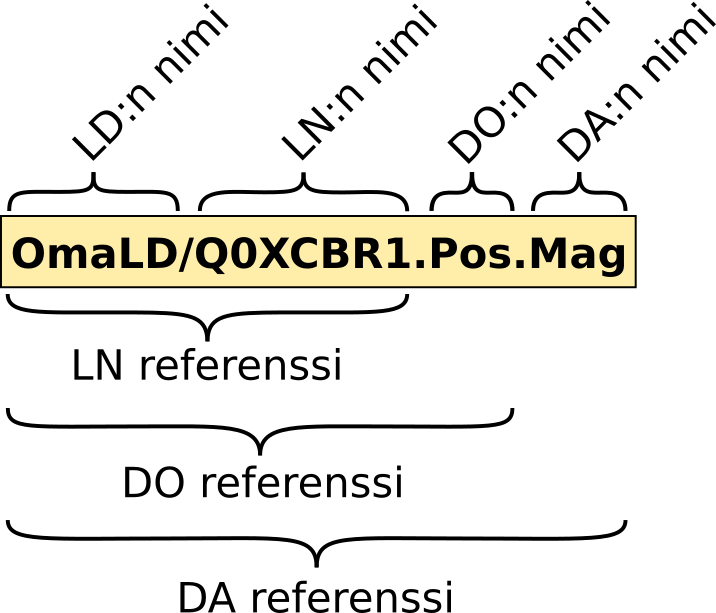
\includegraphics[width=0.5\textwidth]{pictures/iec61850-data-reference.png}
	\caption{IEC 61850 -standardin määrittämä viitteen rakenne.}
	\label{fig:iec61850-data-reference}
\end{figure}

Viite muodostuu suoraan laitteessa olevien luokkien instanssien nimien ja hierarkian mukaan. Loogisen laitteen (LD) ja loogisen noodin (LN) erottimena käytetään kauttaviivaa, ja muiden osien erottimena käytetään pistettä. Loogisella laitteella on aseman insinöörin määrittämä oma nimi, mutta kuitenkin alle 65 merkkiä. Muuten loogisen laitteen nimeen standardi ei puutu. Loogisen noodin instanssin nimi koostuu alku-, keski- ja loppuosasta. Alkuosan käyttäjä voi itse päättää, kuvassa \ref{fig:iec61850-data-reference} Q0. Voi sisältää numeroita ja kirjaimia, mutta täytyy alkaa kirjaimella. Keskiosan täytyy olla loogisen luokan nimi, josta instanssi on tehty. Tässä tapauksessa jo aikaisemmin mainittu katkaisijan luokka, XCBR. Tämä osuus on aina 4 kirjainta pitkä ja on aina isoilla kirjaimilla. Loppuosa on instanssin numeerinen arvo, joka ei sisällä kirjaimia. Loppuosan käyttäjä voi itse päättää, jonka ei tarvitse välttämättä olla juokseva numero. Alku- ja loppuosan yhteenlaskettu merkkien pituus täytyy olla alle 13 merkkiä, eli koko loogisen noodin nimen pituus voi olla maksimissaa 17 merkkiä. Data objektien (DO) ja attribuuttien (DA) niminä käytetään standardin määrittämiä nimiä, jotka määritetään niitä vastaavissa luokissa osissa 7-3 ja 7-4 (katso taulukkot \ref{tab:iec61850-xcbr-class-definition} ja \ref{tab:iec61850-DPC-class-definition}). Riippuen viittauksesta, näistä muodostuu loogisen noodin viite, dataobjektin viite ja data attribuutin viite. Jos data-objektin alla on toinen dataobjekti, jonka alla on vasta itse data-attribuutit. Viittausta vain jatketaan instanssien nimiä liittämällä toisiinsa pisteellä aina data-attribuuttiin asti. Samoin toimitaan kun data-attribuutti on tyypiltään rakennettu tyyppi, kuten Quality, jolla on alidata-attribuutteja. \cite[s.~181--182]{IEC61850-7-2} \cite[s.~93--95]{IEC61850-7-1}

Standardissa määritetään kaksi näkyvyysaluetta (engl. scope) viittaukselle, jotka ovat palvelin- ja looginen laite -näkyvyysalueet. Palvelin tässä yhteydessä tarkoittaa verkkoon kytkettyä laitetta, eli IED-laitetta. Palvelinnäkyvyysalueelle viitataan ottamalla viittauksesta pois loogisen laitteen nimi. Eli kuvassa \ref{fig:iec61850-data-reference} viittaus tulisi muotoon /Q0XCBR1.Pos.stVal. Edellemainittua viittausta käytetään silloin, kun loogisen noodin instanssi sijaitsee loogisen laitteen ulkopuolella, mutta kuitenkin palvelimella. Looginen laite -näkyvyysalueessa viittaus sisältää loogisen laitteen nimen ennen kauttaviivaa, toisin kuin palvelin-näkyvyysalueessa. Esimerkiksi kuvassa \ref{fig:iec61850-data-reference} oleva viittaus OmaLD/Q0XCBR1.Pos.stVal. Loogisen laitteen -näkyvyysaluetta käytetään silloin kun loogisen noodin instanssi sijaitsee loogisen laitteen sisällä sen hierarkiassa. Tässä työssä jatkossa käytetään pelkästään loogisen laitteen -näkyvyysaluetta. \cite[s.~183]{IEC61850-7-2}

Standardi määrittää maksimipituuksia viittauksille. Seuraavaksi kerrotut pituusmääritykset ovat voimassa kummallekin edelle mainitulle näkyvyysalueen viittaukselle. Ennen kauttaviivaa saa olla maksimissaan 64 merkkiä. Tämän jälkeen kauttaviiva, josta seuraa uudelleen maksimissaan 64 merkkiä. Eli koko viittauksen maksimipituus saa olla enintään 129 merkkiä, kauttaviiva mukaan lukien. \cite[s.~24,183]{IEC61850-7-2}


\subsection{Attribuuttien funktionaalinen rajoite ja niistä muodostetut datajoukot}
\label{ch:fc-and-dataset}
Standardin CDC-luokat, määrittävät käytettävät data-attribuutit (katso taulukko \ref{tab:iec61850-DPC-class-definition}). Nämä luokat määrittävät myös jokaiselle data-attribuutille aikaisemmin mainitun funktionaalisen rajoitteen (engl. functional constraint, lyhennetään FC). Funktionaalinen rajoite kuvaa attribuutin käyttötarkoitusta ja sitä mitä palveluita attribuuttiin voidaan käyttää. Esimerkiksi kaikki attribuutit, jotka liittyvät laitteen tilaan (engl. status), niillä on funktionaalinen rajoite ST (standardissa engl. status information). Standardi määrittää paljon erilaisia funktionaalisia rajoitteita, jotka ovat kaikki kahden ison kirjaimen yhdistelmiä. Taulukossa \ref{tab:iec61850-functional-constraints} on esitetty joitain tärkeimpiä funktionaalisia rajoitteita. Funktionaalinen rajoite määrittää myös, onko attribuutti kirjoitettava tai luettava \cite[s.~54]{IEC61850-7-2}.

\begin{table}[ht!]
	\caption{Osa IEC 61850 -standardin määrittämistä funktionaalisista rajoitteitteista (FC).}
	\label{tab:iec61850-functional-constraints}
	\begin{tabular}{l | l | l | l}
		\hline
		\textbf{Lyhenne} & \textbf{Selite} & \textbf{Luettava} & \textbf{Kirjoitettava} \\
		\hline \hline
		ST & Laitteen tilatieto (status) & Kyllä & Ei \\
		MX & Mittaustieto (measurands) & Kyllä & Ei \\
		CF & Laitteen asetusarvo (configuration) & Kyllä & Kyllä \\
		DC & Selitystieto (description) & Kyllä & Kyllä \\
		\hline
	\end{tabular}
\end{table}

Funktionaalista rajoitetta käytetään IED-laitteelle tehtävässä kutsussa viitteen kanssa suodattamaan mitä data-attribuutteja tehty kutsu koskee. Funktionaalinen rajoite on pakollinen tieto kutsuissa, jotka lukevat tai kirjoittavat arvoja. Seuraavaksi esitetään esimerkki kuinka yhdellä kutsulla viitataan moneen data-attribuuttiin. Esimerkkinä otetaan kuvassa \ref{fig:iec61850-data-reference} olevasta viitteestä osa, joka viittaa data-objektiin. Eli OmaLD/Q0XCBR1.Pos, jolloin viite on DO-viite. Kutsun vaikutusalue on aina hierarkiassa alaspäin. Eli nyt viitteellä viitataan Pos-dataobjektin kaikkiin alla oleviin data-attribuutteihin. Katso taulukko \ref{tab:iec61850-DPC-class-definition}, jossa on esitetty kaikki Pos-dataobjektin alla olevat data-attribuutit, johon nyt viitataan. Huomiona, jos viittauksen alla olisi alidata-objekteja, niidenkin data-attribuutit kuuluvat viittauksen piiriin. Viittauksen vaikutuksen voi siis ajatella jatkuvan viittauskohdasta alaspäin rekursiivisesti kaikkiin ali-instansseihin. Funktionaalista rajoitetta käytetään suodattamaan kaikista viitatuista data-attribuuteista ne, jotka halutaan kirjoittaa tai lukea. Esimerkkinä jos kutsuun viitteellä OmaLD/Q0XCBR1.Pos lisättäisiin funktionaalinen rajoite ST. Rajoitettaisiin kutsu koskemaan Pos-dataobjektin alidata-attribuuteista vain niitä attribuutteja, joilla on funktionaalinen rajoite ST. Eli taulukon \ref{tab:iec61850-DPC-class-definition} mukaan attribuutit olisivat origin, ctlNum, stVal, q, t ja stSeld. Muut data-attribuutit suodatetaan pois kutsun vaikutuksesta. Sama suodatus tapahtuu rekursiivisesti hierarkiassa alaspäin kaikille alidata-attribuuteille. Esimerkissä olevat arvot voisi vain lukea, ei kirjoittaa. Tämä sen takia, että taulukon \ref{tab:iec61850-functional-constraints} mukaan funktionaalinen rajoite ST sallii vain lukemisen. IEC 61850 -standardissa määritetään funktionaalinen rajoite XX, joka on sama kuin mikä tahansa muu funktionaalinen rajoite. Kuitenkin standardin osassa 8-1 joka tekee toteutuksen MMS-protokollalle, tämä ei ole tuettu toiminnalisuus. Eli toisin sanoen, jos MMS-protokollan kanssa halutaan lukea kaikki yhden data-objektin data-attribuutit. Joudutaan tekemään kutsu jokaista data-objektin funktionaalista rajoitetta kohti.

Viittauksen ja funktionaalisen rajoitteen avulla siis suodatetaan rekursiivisesti hierarkiassa alaspäin olevia data-attribuutteja. IEC 61850 -standardissa on määritelty nimitykset käytettäväksi kun jotakin viittausta suodatetaan funktionaalisella rajoitteella. Nämä ovat FCD (engl. functional constrained data) ja FCDA (engl. functional constrained data attribute). Nämä nimitykset ovat standardissa vain käsite, joka ei toteudu mitenkään tekniikalla. Taulukossa \ref{tab:fcd-ja-fcda} on esitetty viittauksia eri tyyppisiin instansseihin funktionaalisella rajoitteella. Taulukosta selviää viitattu instanssi dataobjekti (DO) tai data-attribuutti (DA), instanssin tyyppi ja käytetty nimitys viittaukselle FCD tai FCDA. FCD nimitys on silloin kun vain hierarkian ensimmäistä dataobjekti rajoitetaan funktionaalisesti. FCDA nimitys on käytössä kaikille muille viittauksille hierarkiassa alaspäin, joita rajoitetaan funktionaalisesti. Huomaa taulukossa \ref{tab:fcd-ja-fcda} viittaus OmaLD/MMXU1.PhV.phsA, joka viittaa PhV dataobjekin alidataobjektiin. Tämä on FCDA-viittaus, vaikka kyseessä onkin dataobjekti. Ainoa ero FCD:n ja FCDA:n nimitysten välillä on vain se, että FCD-viittaus on aina vain hierarkian ensimmäiseen dataobjektiin ja FCDA-viittaus siitä eteenpäin hierarkiassa. Riippumatta mitä tyyppejä viitatut instanssit hierarkiassa alaspäin ovat. \cite[s.~55]{IEC61850-7-2} \cite[s.~63]{IEC61850-8-1}

\begin{table}[ht!]
	\caption{Viitteen nimeäminen lyhenteellä funktionaalisen rajoitteen kanssa.}
	\label{tab:fcd-ja-fcda}
	\begin{tabular}{l | l | l | l | l}
		\hline
		\textbf{FC} & \textbf{Viite} & \textbf{Instanssi} & \textbf{Tyyppi} & \textbf{Nimitys} \\
		\hline \hline
		ST & OmaLD/XCBR1.Pos & DO & DPC & FCD \\
		ST & OmaLD/XCBR1.Pos.t & DA & TimeStamp & FCDA \\
		ST & OmaLD/XCBR1.Pos.ctlNum & DA & INT8U & FCDA \\
		MX & OmaLD/MMXU1.PhV & DO & WYE & FCD \\
		MX & OmaLD/MMXU1.PhV.phsA & DO & CMV & FCDA \\
		MX & OmaLD/MMXU1.PhV.phsA.t & DA & TimeStamp & FCDA \\
		\hline
	\end{tabular}
\end{table}

Funktionaalista rajoitetta käytetään viitteen kanssa suodattamaan viitatusta kohdasta alaspäin kaikki data-attribuutit. Tätä toiminnallisuutta käytetään hyväksi, kun tehdään kirjoittavia tai lukevia kutsuja ja rajoitetaan kutsulla vaikutettavia data-attribuutteja. Tätä samaa mekanismia käytetään hyväksi kun IED-laitteeseen määritellään datajoukkoja. IEC 61850 -standardissa datajoukko koostuu joukosta IED-laitteessa olemassa olevista data-attribuuteista. Datajoukko on tapa koostaa yhteen kiinnostavat data-attribuutit IED-laitteelta. Datajoukko nimetään ja sijoitetaan IED-laitteen hierarkiaan. Näin siihen voidaan viitata kutsuilla kuten mihin tahansa muuhun hierarkian instanssiin. Datajoukot IED-laitteelle rakennetaan käyttämällä FCD ja FCDA viitteitä. Datajoukko koostuu siis joukosta FCD- ja FCDA -viitteitä. Jokaisella viitteellä on jokin funktionaalinen rajoite, joka suodattaa viitteen alla olevat attribuutit ja sisällyttää ne kyseiseen datajoukkoon. Esimerkkinä datajoukon rakentamisesta taulukon \ref{tab:fcd-ja-fcda} viittet. Näistä viitteistä voitaisiin rakentaa oikea standardin mukainen datajoukko, nimetä se nimellä Testi1, ja lisätä IED-laitteen hiearkiaan kohtaan OmaLD/LLN0.Testi1. Nyt datajoukkoon voisi viitata ja vaikka lukea kaikki sen arvot yhdellä kertaa. Jotta datajoukko saadaan näin tehtyä, tieto tästä pitäisi lisätä IED-laitteen asetustiedostoon. Datajoukkoja IED-laitteessa käytetään muodostamaan joukkoja tärkeistä data attribuuteista, joita voidaan esimerkiksi lukea ja kirjoittaa yhdellä kutsulla. Datajoukkoja käytetään myös tilattavien viestien sisältönä. Viestejä voi standardin mukaan tilata vain datajoukoista olevista data-attribuuteista. \cite[s.~61--68]{IEC61850-7-2}


\subsection{Viestien tilaus ja tilauksen konfigurointi}
\label{ch:viestien-tilaus-ja-tilauksen-konfigurointi}
IEC 61850 -standardi määrittää, kuinka IED-laitteen ulkopuolinen ohjelma voi tilata kiinnostavien data-attribuuttien arvoja verkon yli. Viesti voidaan esimerkiksi lähettää tilaajelle, kun mitatun jännitteen arvo muuttuu. Kyseessä on tilaaja-julkaisija arkkitehtuurimalli, jossa ulkopuolinen ohjelma on tilaaja ja IED-laite julkaisuja. Standardi määrittää, että viestejä voidaan tilata vain datajoukoissa viitatuilla data-attribuuteilta. Milloin viestin lähetys tilaajalle tapahtuu, riippuu siitä kuinka tilaaja liipaisimet asettaa tilauksen yhteydessä. Standardissa määritellään käytettäväksi erilaisia liipaisimia joilla tilaaja voi muokata millä ehdoilla viesti pitäisi lähettää. Standardissa on myös määritetty mekanismit, jolla tilajaa voi pyytää kaikki arvot kerralla tai tilata jaksottaisia viestejä tietyn aikavälein.

Standardissa määritetään luokka, jonka tehtävä on hoitaa tilausta ja sen asetuksia. Tässä kappaleessa käydään läpi luokan yleistä toiminnallisuutta, kappaleessa \ref{rcb-toiminta} käsitellään luokan attribuutteja ja toimintaa syvällisemmin. Niinkuin muutkin luokat standardissa, tästä tehdään instanssi, sille annetaan yksilöivä nimi ja se lisätään IED-laitteen hierarkiaan. Nämä määritellään IED-laitteen asetustiedostossa, kuten kaikki muutkin instanssit. Yksilöivän nimen avulla tilaaja voi viitata kutsulla instanssiin, muuttaa luokan asetuksia ja aloittaa tilauksen. Nämä luokat standardissa ovat puskuroitu viestintäluokka (engl. Buffered Report Control Block, lyhennetään BRCB) ja ei puskuroitu luokka (engl. Unbuffered Report Control Block, lyhennetään URCB). Tekstissä kumpaakin luokkaan viitatessa käytetään lyhennettä RCB. Ainoa ero luokkien toiminnan välillä on, että BRCB puskuroi viestejä jonkin aikaa yhteyden katkettua. Yhteyden palautuessa, se lähettää puskuroidut viestit järjestyksessä asiakkaalle. BRCB takaa viestien järjestyksen ja saatavuuden. URCB lähettää viestejä asiakkaalle ilman puskurointia ja yhteyden katketessa, viestit menetetään. Standardissa määritetään, että yksi RCB-instanssi voi palvella vain yhtä tilaaja kerrallaan. IED-laitteeseen täytyy määrittää instansseja sen tilaajien määrän mukaan.

Kuvassa \ref{fig:iec61850-brcb-communication} on esitetty tilaajan ja IED-laitteen välinen viestien tilauksen prosessi. Kuvassa ensin asiakas tilaa puskuroidun BRCB-instanssin. Ensimmäisessä kutsussa tilaaja kirjoittaa RCB-luokan arvot, kuten käytettävät liipaisimet jne. Kutsussa tilaajan on merkittävä RCB-instanssin varatuksi, jotta tilaus käynnistyy. IED-laite aloittaa viestien julkaisun tilaajalle määritettyjen ehtojen mukaan. Jos tilaaja ja IED-laitteen välinen yhteys katkeaa, BRCB-intanssi puskuroi viestejä johonkin järkevään rajaan asti. Kun yhteys tilaajan palaa, IED lähettää viestit järjestyksessä tilaajalle alkaen ensin puskurista. Tilaaja voi lopettaa tilauksen ja instanssin varauksen merkitsemällä sen taas vapaaksi.

\begin{figure}[ht!]
	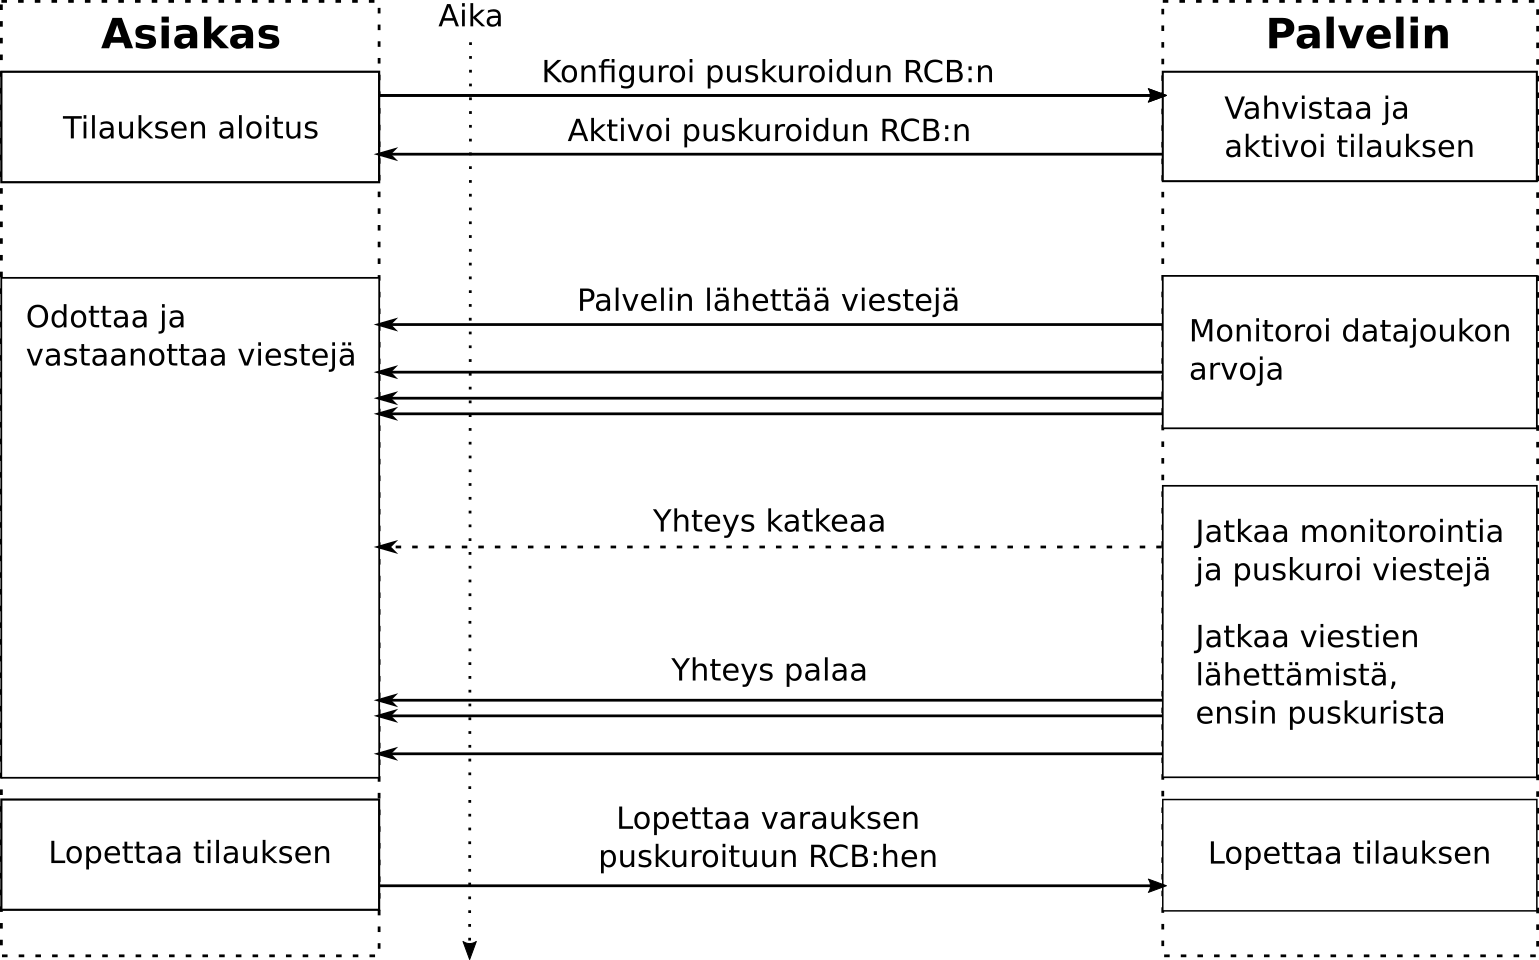
\includegraphics[width=1\textwidth]{pictures/iec61850-brcb-communication.png}
	\caption{Puskuroitu viestien tilausprosessi tilaajan ja IED-laitteen välillä.}
	\label{fig:iec61850-brcb-communication}
\end{figure}

Standardissa määritetään, että viestejä voidaan tilata vain datajoukoista. IED-laitteen asetustiedostossa täytyy myös määrittää mitä datajoukkoa RCB-intanssi käyttää. Tämän jälkeen instanssi tarkkailee datajoukkon attribuuttien muutoksia ja lähettää viestin, jos tilaajan asettama liipaisin täsmää. Koska yksi RCB voi palvella vain yhtä tilaajaa kerrallaan, täytyy samaan datajoukkoon viitata monella eri RCB-instanssilla. Näin monta eri tilaajaa saavat viestin samasta tapahtumasta.

Standardissa on määritetty seuraavat liipaisimet data-attribuuteille, joita RCB tarkkailee ja reagoi:
\begin{itemize}
	\item datan muutos (engl. data change, standardissa lyhenne dchg),
	\item laadun muutos (engl. quality change, standardissa lyhenne qchg), ja
	\item datan päivitys (engl. data update, standardissa lyhenne dupd).
\end{itemize}
Jokaiselle data-attribuutille määritellään erikseen mitä liipaisimia se tukee. Nämä määritellään standardin luokkien määrityksissä. Esimerkkinä aikaisemmin mainittu DPC-luokan määritys taulukossa \ref{tab:iec61850-DPC-class-definition}, jossa TrgOp-sarake kertoo attribuutin liipaisimen. Data muutos ja päivitys liipaisimen ero on, että datan päivitys liipaisee tapahtuman vaikka attribuutin uusi arvo olisi sama. Datan muutos ei liipaise tapahtumaa, jos uusi arvo on sama kuin edellinen arvo. Laadun muutos liipaisin tarkoittaa, että data attribuuttiin liitetty laatuarvo muuttui. Laatuarvo kertoo tilaajalle ja arvojen lukijalle, voiko attribuutien arvoihin luottaa. Laatuarvo on tyyppiä Quality ja tästä voi tarvittaessa lukea enemmän standardista. \cite[s.~90]{IEC61850-7-1}


\subsection{Raportointi-luokan määritys ja toiminta}
\label{rcb-toiminta}
BRCB-luokalla on erilaisia attribuutteja, joita tilaaja voi kirjoittaa ja lukea ennen tilauksen aloittamista. BRCB ja URCB -luokat eivät eroa paljon attribuuteilla toisistaan, joten tässä kappaleessa keskitytään vain BRCB-luokan toimintaan. Tarkka määritys luokkien eroista löytyy standardin osasta 7-2. Taulukossa \ref{tab:iec61850-brcb-class-definition} on esitetty standardin määrittämän BRCB-luokan attribuutit, attribuutin nimi englanniksi ja sen selite. Taulukossa ei ole esitetty attribuuttien tyyppejä, koska ne voi lukija tarvittaessa tarkemmin lukea standardin omasta määrityksestä. Lisäksi tässä kappaleessa käydään läpi luokan atrribuuttien toiminta pääpiirteittäin ja loput tiedot lukija voi tarkistaa standardista. \cite[s.~93--118]{IEC61850-7-2}.

\begin{table}[ht!]
	\caption{BRCB-luokan määritetyt attribuutit ja niiden selitteet.}
	\label{tab:iec61850-brcb-class-definition}
	\begin{tabular}{l | l | l}
		\hline
		\textbf{Attribuutti} & \textbf{Englanniksi} & \textbf{Selite} \\
		\hline \hline
		BRCBName & BRCB name & Objektin nimi \\
		&\\
		BRCBRef & BRCB reference & Objektin viite \\
		&\\
		RptID & Report identifier & \parbox[t]{7.5cm}{RCB-instanssin yksilöivä id lähetettyihin viesteihin, asiakas voi asettaa} \\
		&\\
		RptEna & Report enable & Varaa RCB:n ja aloittaa viestien lähetyksen \\
		&\\
		DatSet & Data set reference & Tarkailtavan datajoukon viite \\
		&\\
		ConfRev & Configuration revision & \parbox[t]{7.5cm}{Juokseva konfiguraation numerointi, muutos kasvattaa numerointia} \\
		&\\
		OptFlds & Optional fields & Mitä valinnaisia kenttiä viestiin lisätään \\
		&\\
		BufTm & Buffer time & \parbox[t]{7.5cm}{Puskurointiaika, ennen viestin lähetystä. Tänä aikana tapahtuvat liipaisut yhdistetään samaan viestiin} \\
		&\\
		SqNum & Sequence number & Juokseva lähetetyn viestin numerointi \\
		&\\
		TrgOps & Trigger options & Millä liipaisimilla viesti lähetetään \\
		&\\
		IntgPd & Integrity period & \parbox[t]{7.5cm}{Periodisen viestien väli millisekunteina, arvolla 0 ei käytössä} \\
		&\\
		GI & General-interrogation & \parbox[t]{7.5cm}{Käynnistää yleiskyselyn, joka sisältää kaikki datajoukon attribuutit seuraavaan viestiin} \\
		&\\
		PurgeBuf & Purge buffer & Puhdistaa lähettämättömät viestit puskurista \\
		&\\
		EntryID & Entry identifier & \parbox[t]{7.5cm}{Puskurissa olevan viimeisimmän viestin id. Arvo 0 tarkoittaa tyhjää puskuria} \\
		&\\
		TimeOfEntry & Time of entry & \parbox[t]{7.5cm}{Puskurissa olevan viimeisimmän viestin aikaleima} \\
		&\\
		ResvTms & Reservation time & \parbox[t]{7.5cm}{Instanssin varausaika sekunteina kun yhteys katkeaa, arvo -1 tarkoittaa konfiguraation aikaista varausta ja 0 että ei varausta} \\
		&\\
		Owner & Owner & \parbox[t]{7.5cm}{Yksilöi varaavan asiakkaan, yleensä IP-osoite tai IED-laitteen nimi. Arvo 0 että RCB on vapaa tai ei omistajaa} \\
		\hline
	\end{tabular}
\end{table}

Tilaaja voi vapaasti RCB-instanssin arvoja kirjoittaa ja lukea ennen tilauksen aloittamista monella peräkkäisellä kutsulla. Tärkein attribuutti luokassa on RptEna, joka on boolean tyyppiä. Kun attribuutti kirjoitetaan arvoon tosi, aloittaa instanssi tilauksen ja varaa sen tilaajalle. Tilauksen ollessa päällä, tilaaja voi edelleen lukea ja kirjoittaa sen arvoja, mutta rajoitetusti. Joidenkin arvojen kirjoitus pitää tapahtua ennen tilausta tai samassa kutsussa kun RtpEna asetetaan arvoon tosi. Tilaaja lopettaa tilauksen jos yhteys on poikki tarpeeksi kauan tai RptEna kirjotetaan arvoon epätosi.

RCB-luokan TrgOps-attribuutti on binääritietue, jossa yksittäinen bitti ilmaisee mikä liipaisin aiheuttaa viestin lähettämisen. Tällä attribuutilla tilaaja voi päättää mitä liipaisimia hän haluaa käyttää. TrgOps sisältää seuraavat liipaisimet:
\begin{itemize}
	\item datan muutos (engl. data change, standardissa lyhenne dchg),
	\item laadun muutos (engl. quality change, standardissa lyhenne qchg), ja
	\item datan päivitys (engl. data update, standardissa lyhenne dupd),
	\item yleinen kysely (enlg. general-interrogation, standardissa lyhenne GI), ja 
	\item jatkuva viestintä väliajoin (engl. intergrity).
\end{itemize}

Kolme ensimmäistä liipaisinta dchg, qchg ja dupd ovat aikaisemmin kappaleessa \ref{ch:viestien-tilaus-ja-tilauksen-konfigurointi} määrittettyjen data attribuuttien liipaisimia. Asiakas voi tilata viestejä esimerkiksi vain datan muutoksista ja ei muista. RCB-luokka määrittää data attribuuttien liipaisimien lisäksi vielä kaksi liipaisinta lisää, yleinen kysely ja jatkuva viestintä väliajoin. Yleinen kysely on viesti, johon RCB sisällyttää kaikki datajoukon attribuutit. Asiakas voi liipaista sen asettamalla luokan attribuutin GI arvoksi tosi ja TrgOps attribuutissa liipaisin on päällä. Tällöin RCB käynnistää viestin generoinnin ja lähettää sen asiakkaalle. Jos liipaisin ei ole päällä TrgOps attribuutissa, ja GI arvoksi asetetaan tosi. RCB ei generoi viestiä. Viestin lähetyksen jälkeen RCB itse asettaa GI:n arvoksi epätosi. Jatkuva viestintä liipaisin on jatkuvaa viestin lähettämistä tilaajalle väliajoin, johon sisältyy kaikki datajoukon attribuutit, kuten yleisessä kyselyssä. Toiminnon saa päälle kun asiakas asettaa RCB-luokassa attribuutit IntgPd arvoksi muu kuin 0, ja TrgOps-attribuutin arvossa kyseinen liipaisin on päällä. Attribuutti IntgPd kertoo minkä väliajoin viesti generoidaan ja lähetetään asiakkaalle. Jos IntgPd arvo on muu kuin 0 ja TrgOps attribuutissa liipaisin ei ole päällä, ei viestiä generoida ja lähetetä asiakkaalle väliajoin.

RCB-luokan attribuuttin OptFlds avulla asiakas voi valita mitä vaihtoehtoisia kenttiä viestiin sisällytetään. Attribuutin OptFlds on binääritietue niin kuin ja TrgOps. Taulukossa \ref{tab:iec61850-optional-fields-definition} on esitetty sen asetettavat arvot \cite[s.~98]{IEC61850-7-2}. Taulukon yksittäinen kenttä vastaa OptFlds arvon yhtä bittiä. Bittien järjestys määräytyy tekniikalle toteutuksen perusteella. Esimerkiksi MMS-protokolla. Taulukon arvoilla tilaaja voi määrittää mitä lisätietoa viestiin sisällytetään. Esimerkiksi asettamalla reason-for-inclusion bitin päälle, liitetään viestin arvon yhteyteen miksi tämä arvo viestiin sisällytettiin. Viestin rakennetta ja kuinka OptFlds-attribuutin arvoilla sen sisältöön voi vaikuttaa käydään läpi tarkemmin kappaleessa \ref{ch:viestin-rakenne}.

\begin{table}[ht!]
	\caption{RCB-luokan OptFlds-attribuutin arvot ja niiden selitteet.}
	\label{tab:iec61850-optional-fields-definition}
	\begin{tabular}{l | l}
		\hline
		\textbf{Arvo} & \textbf{Selite} \\
		\hline \hline
		sequence-number & Jos tosi, sisällytä RCB-luokan attribuutti SqNum viestiin \\
		report-time-stamp & Jos tosi, sisällytä RCB-luokan attribuutti TimeOfEntry viestiin \\
		reason-for-inclusion & Jos tosi, sisällytä syy miksi arvo(t) sisällytettiin viestiin \\
		data-set-name & Jos tosi, sisällytä RCB-luokan attribuutti DatSet viestiin \\
		data-reference & \parbox[t]{10cm}{Jos tosi, sisällytä datajoukon liipaisseen kohdan rakentamiseen käytetty FCD- tai FCDA-viite viestiin} \\
		buffer-overflow & \parbox[t]{10cm}{Jos tosi, sisällytä viestiin tieto onko puskuri vuotanut yli kentällä BufOvfl (engl. buffer overflow)} \\
		entryID & Jos tosi, sisällytä RCB-luokan attribuutti EntryID viestiin \\
		conf-revision & Jos tosi, sisällytä RCB-luokan attribuutti ConfRev viestiin \\
		\hline
	\end{tabular}
\end{table}

Lähetetyt viestit voivat sisältää vaihtelevan määrän sisällytettyjä arvoja. RCB-instanssi mittaa aikaa ensimmäisestä liipaisusta sen attribuutin BufTm verran ja tämän ajan jälkeen pakkaa kaikki liipaisseet attribuutit samaan viestiin. Tilaaja voi muuttaa arvoa jos haluaa käyttää pitempää tai lyhyempää puskurointiaikaa.


\subsection{Viestin rakenne ja kuinka sen sisältö muodostuu}
\label{ch:viestin-rakenne}
IED:n lähettämä viesti on rakenteeltaan hiukan monimutkainen ja lisäksi siihen vaikuttaa RCB-instanssin OptFlds-attribuutin asetetut bitit (taulukko \ref{tab:iec61850-optional-fields-definition}). Tässä kappaleessa käsitellään viestin mallia, joka on tekniikasta riippumaton. Minkälainen viestin rakenne on MMS-protokollan tasolla, siitä ei tarvitse välittää. Toteutetussa ohjelmassa käytettiin kirjastoa, joka hoitaa matalan tason asiat ja tarjoaa helppokäyttöisen rajapinnan viestin sisältöön. Kuitenkin viestin rakenteesta täytyy ymmärtää kuinka vaihtoehtoiset kentät siihen vaikuttavat ja kuinka attribuuttien arvot viestiin sisällytetään. Kuvassa \ref{fig:iec61850-report-format} on esitetty standardin määrittämän viestin rakenne ja mitä kenttiä OptFlds-attribuutti kontrolloi. Viestin rakenteen voisi ajatella koostuvan kahdesta osasta. Ensin viestissä on yleinen tieto ja viimeisenä taulukko datajoukon alkioista 1--n:ään, jotka liipaisevat viestin lähetyksen.

\begin{figure}[ht!]
	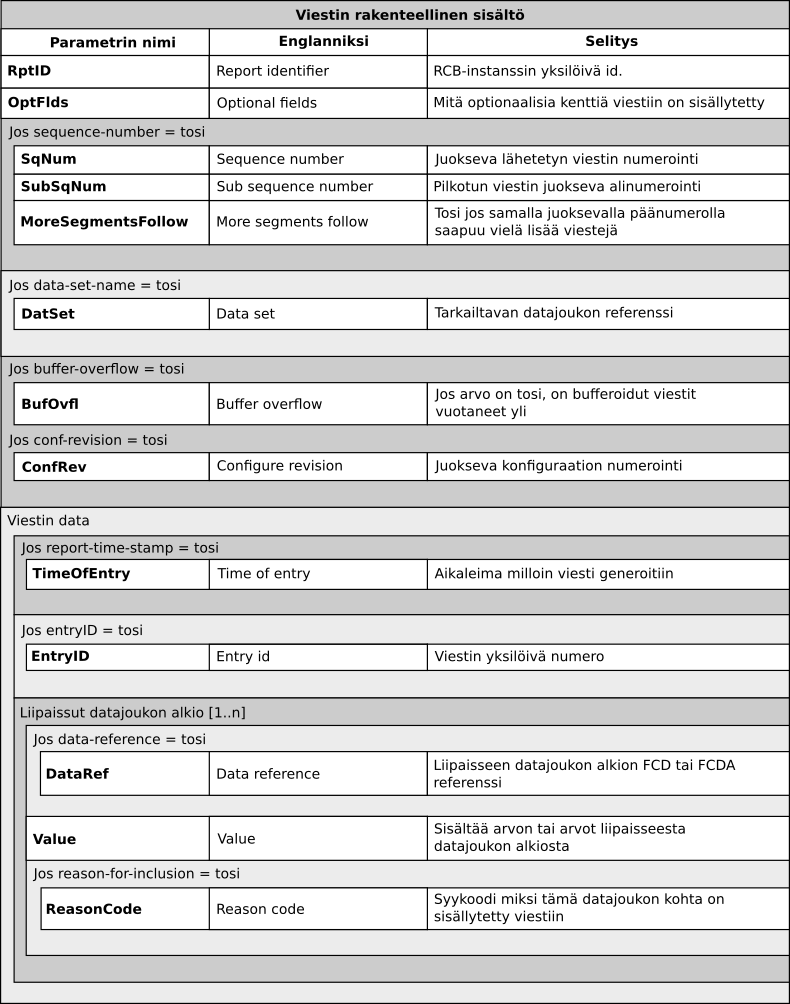
\includegraphics[width=1\textwidth]{pictures/iec61850-report-format.png}
	\caption{Standardin määrittämä lähetetyn viestin rakenne (pohjautuu kuvaan \cite[s.~104]{IEC61850-7-2}).}
	\label{fig:iec61850-report-format}
\end{figure}

Kuvassa \ref{fig:iec61850-data-set-reporting} on esitetty yleinen kuva kahden viestin lähetyksestä liipaisun tapahtuessa. Kuvassa keskellä on kaksi BRCB-instanssia myBRCB01 ja myBRCB02, jotka tarkkailevat datajoukkoja Testi1 ja Testi2 vastaavasti. Kummatkin instanssit lähettävät viestin, jotka ovat kuvassa oikealle. BRCB-instansseista voi nähdä, mitä niille asetetut attribuuttien arvot ovat ja datajoukoista näkee mistä FCD- ja FCDA -viitteistä ne koostuvat. Kuvassa attribuutin MyLD/XCBR1.Pos.stVal arvo muuttuu ja tämä liipaisee viestin lähetyksen kummassakin BRCB-instanssissa. Viesteistä voi nähdä sen sisällön ja myös miten BRCB-instanssien OptFlds-attribuutin arvot vaikuttavat sen sisältöön. Lähetettyjen viestien rakennetta ja sisältöä voi verrata kuvassa \ref{fig:iec61850-report-format} määritetyn viestin rakenteeseen. Kuvassa on esitetty myös kuinka BRCB-instansseihin viitataan MMS-protokollan tapauksessa. Tätä käsitellään tarkemmin kappaleessa \ref{ch:iec61850-mms-mallinnus}.

\begin{figure}[ht!]
	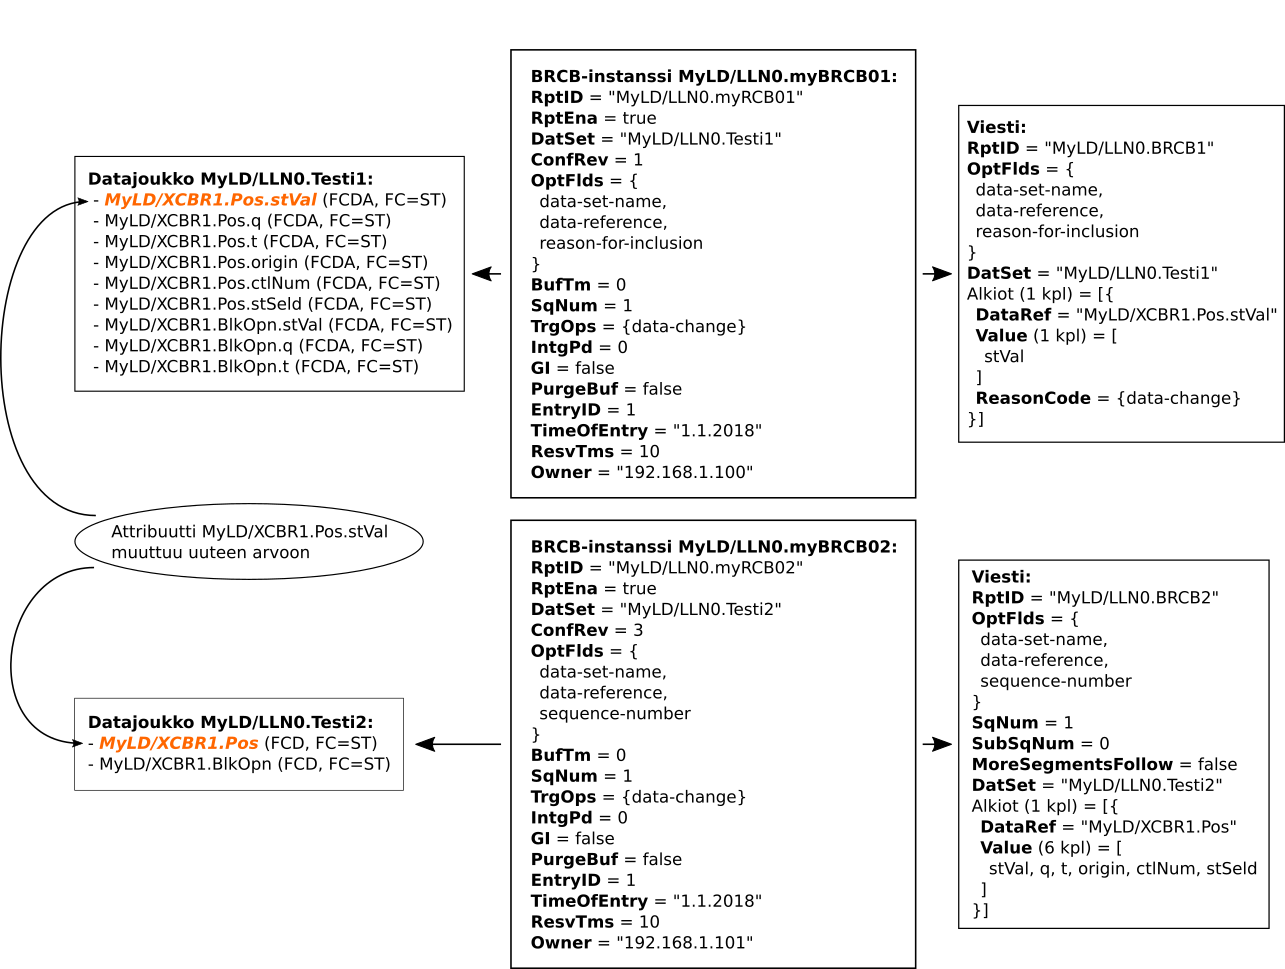
\includegraphics[width=1\textwidth]{pictures/iec61850-data-set-reporting.png}
	\caption{BRCB-instanssi tarkkailee sille määritettyä datajoukoa ja generoi viestin tapahtuman liipaistessa.}
	\label{fig:iec61850-data-set-reporting}
\end{figure}

Viestissä kenttä RptID sisältää viitteen RCB-instanssiin, mistä viestin on peräisin. OptFlds sisältää binääritietueen viestin vaihtoehtoisista kentistä. Tämä kenttä on suoraan verrattavissa viestin kenttiä SqNun, SubSqNum ja MoreSegmentsFollow käytetään kertomaan asiakkaalle, jos päätason viesti on liian pitkä ja se on pilkottu alaosiin. Kenttä SqNum on RCB-instanssin samanniminen kenttä ja on juokseva numerointi päätason viesteille. Kenttä SubSqNum on juokseva numerointi alkaen 0, mikäli kyseessä on päätason viesti, eli saman SqNum arvon sisältävä viesti on pilkottu osiin. Kentän MoreSegmentsFollow ollessa tosi asiakas tietää että päätason viesti on pilkottu osiin ja seuraava osa on odotettavissa palvelimelta. Kun viestin kaikki osat on lähetetty, palvelin asettaa viimeisessä viestissä kentän MoreSegmentsFollow arvoksi epätosi ja seuraavassa päätason viestissä SubSqNum kentän arvoksi 0. Kenttä DatSet sisältää viitteen datajoukkoon mistä viestin on peräisin. Puskuroidussa BRCB-instanssissa kenttä BufOvlf kertoo onko viestipuskuri vuotanut yli. ConfRev kertoo juoksevan konfiguraation numeron, tämä tulee suoraan RCB-instanssin samannimisestä attribuutista. TimeOfEntry kertoo milloin viesti generoitiin IED-laitteen päässä. EntryID on viestin yksilöivä numerointi. Tämä kenttä tulee suoraan RCB-instanssin samannimisestä kentästä. Tämän jälkeen viestissä tulee taulukko, joka sisältää liipaisseet datajoukon alkiot. Jokainen taulukon alkio sisältää Value-kentän ja vaihtoehtoiset DataRef ja ReasonCode kentät. DataRef sisältää datajoukon FCD- tai FCDA-viitteen, joka liipaisi tapahtuman. ReasonCode kenttä kertoo mikä RCB-instanssin TrgOps-attribuutilla asetetuista liipaisimista liipaisi tapahtuman ja aiheutti alkion sisällytyksen viestiin. Kentän mahdolliset arvot ovat samat kuin RCB-instanssin TrgOps-attribuutin arvot.

Value-kentän arvosta on tärkeä ymmärtää, että se voi sisältää yhden tai monta data-attribuutin arvoa. Tämä riippuu viittaako datajoukon liippaissut alkion FCD- vai FCDA-viitteellä useaan data-attribuuttiin. Viittauksen ollessa FCDA-viite, joka viittaa vain yhteen data-attribuutiin, sisältää Value-kenttä vain kyseisen data attribuutin arvon. Jos viittaus on FCD- tai FCDA-viite joka viittaa moneen attribuuttiin hierarkiassa alaspäin. Viittaus sisältää Value-kenttä kaikki nämä viitatut arvot, vaikka niistä olisi liipaissut vain yksi attribuutti. FCD- ja FCDA-viittauksen toimintaa ja mitä attribuutteja se viittaa hierarkiassa alaspäin, käydään läpi kappaleessa \ref{ch:fc-and-dataset}. Esimerkki tästä on kuvassa \ref{fig:iec61850-data-set-reporting}, jossa liipaisu yhdessä attribuutissa aiheuttaa eri määrän arvoja kumpaankin viestiin. Tähän vaikuttaa kuinka liipaisevaan attribuuttiin on viitattu datajoukossa. Kuvassa datajoukossa Testi1 attribuuttiin MyLD/XCBR1.Pos.stVal on viitattu FCDA-viitteellä, jossa funktionaalinen rajoite on ST. Eli FCDA-viite viittaa vain stVal attribuuttiin, ei muihin. Tämän takia myBRCB01-instanssilta tuleva viestin Value-kenttä sisältää vain stVal-attribuutin arvon. Kun taas datajoukossa Testi2 attributtiin MyLD/XCBR1.Pos.stVal sisältyy datajoukon ensimmäiseen FCD-viitteeseen funktionaalisella rajoitteella ST. Koska FCD-viite viittaa kaikkiin Pos-instanssin alla oleviin attribuutteihin, joilla funktionaalinen rajoite on ST. Lisätään kaikki nämä attribuutit viestiin, joka lähetetään tilaajalle. BRCB-instansilta myBRCB02 tuleva viestin Value-kenttä sisältää kaikki viitatut attribuutit ja viestin DatRef-kenttä sisältää datajoukossa käytetyn viitteen. Dataobjektin Pos kaikki attribuutit voi tarkistaa taulukosta \ref{tab:iec61850-DPC-class-definition}. \cite[s.~40--44]{IEC61850-7-1} \cite[s.~108]{IEC61850-7-2}


\subsection{Abstraktimallin sovitus MMS-protokollaan}
\label{ch:iec61850-mms-mallinnus}
Tähän asti käsitellyt IEC 61850 -standardin mallit ja palvelut ovat olleet abstrahoituja ja tekniikasta riippumattomia. Tässä työssä käytetiin IEC 61850 -standardin MMS-protokollan toteutusta (engl. Manufacturing Message Specification). Tästä toteutuksesta on tarkemmin määritetty IEC 61850 -standardin osassa 8-1. MMS-protokolla on maailmanlaajuinen ISO 9506 -standardi viestintään, joka on määritetty toimivaksi TCP/IP:n pinon päällä \cite{MMS-protocol-stack-and-API}. Tämän työn kannalta lukijan ei ole tarvitse ymmärtää MMS-protokollaa ja sen toimintaa. Suunnitellussa ohjelmistossa käytettiin apuna kirjastoa, joka hoitaa matalan tason kommunikoinnin IED-laitteen kanssa. Tässä osiossa käsitellään työn kannalta tärkeitä tietoja, mitä toteutksesta MMS-protokollalle kuitenkin tarvitsee tietää. \cite{Introduction-to-the-MMS}

IEC 61850 -standardin mallinnuksessa aikaisemmin esitetty instanssien viittaus hierarkiassa muuttuu ja nyt viittaus sisältää myös funktionaalisen rajoitteen. Esimerkkinä kuvassa \ref{fig:iec61850-data-reference} oleva viite "OmaLD/Q0XCBR1.Pos.stVal" funktionaalisella rajoitteella ST, muuttuu muotoo "OmaLD/Q0XCBR1\$ST\$Pos\$stVal". Tässä viittauksessa pisteet (.) korvataan dollari-merkillä (\$). Ja kaksikirjaiminen funktionaalinen rajoite sijoitetaan loogisen noodin ja ensimmäisen data objektin nimien väliin. Muuten viittaus säilyy identtisenä alkuperäiseen ja samat rajoitteet ja nimeämiskäytännöt ovat voimassa edelleen. \cite[s.~34--35, 111]{IEC61850-8-1}

Tämän uuden viittauksen takia jokaiselle viitattavalle kohteelle täytyy olla funktionaalinen rajoite. Niinpä esimerkiksi RCB-luokkien instansseille täytyy olla myös funktionaalinen rajoite. Puskuroitua RCB-instanssia viitataan funktionaalisella rajoitteella BR. Ja puskuroimatonta funktionaalisella rajoitteella RP. Esimerkin tästä viittauksesta voi nähdä aikaisemmin mainitusta kuvasta \ref{fig:iec61850-data-set-reporting}. \cite[s.~32--34, 75]{IEC61850-8-1}


\section{Advanced Message Queuing Protocol (AMQP)}
Työssä toteutetussa ohjelmistossa IED-laitteelta verkon yli tilatut viestit ohjelma prosessoi ja lähetti viestin eteenpäin välittäjälle (engl. message broker). Välittäjä on verkossa oleva erillinen palvelin, mistä muut ohjelmat pystyivät tilaamaan viestejä tarpeidensa mukaan. Kuvassa \ref{fig:implemented-system-communication} on esitetty lopullisen toteutuksen tietoliikenne eri osapuolten välillä. Tässä työssä toteutettu ohjelmisto on merkitty kuvaan katkoviivalla. Toteutuksessa oli kyse julkaisu ja tilaus -arkkitehtuurimallista (engl. publish-subscribe pattern), jossa työn toteutettu ohjelmisto oli tilaaja yhdeltä IED-laitteelta ja julkaisija välityspalvelimelle. Ja välityspalvelimen toisessa päässä olevat ohjelmistot olivat tilaajia. Tässä teoriaosuudessa perehdytään viestien välittäjän teoriaan, ja mitä siitä täytyy tietää ohjelmistokehityksen kannalta.

\begin{figure}[ht!]
	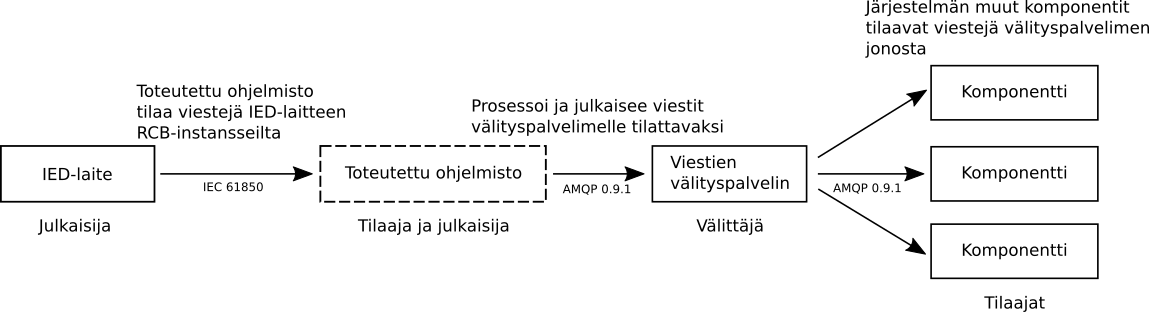
\includegraphics[width=1\textwidth]{pictures/implemented-system-communication.png}
	\caption{Toteutetun ohjelmiston osuus ja rooli käytettävässä kokonaisuudessa tietoliikenteen kannalta.}
	\label{fig:implemented-system-communication}
\end{figure}

Työssä välittäjänä käytettiin RabbitMQ-ohjelmistoa\footnote{\url{https://www.rabbitmq.com/}}, joka on avoimen lähdekoodin välittäjäpalvelin ja perustuu avoimeen AMQP-standardiin\footnote{\url{https://www.amqp.org/}} (engl. Advanced Message Queuing Protocol). AMQP määrittää yhteisen protokollan viestintään eri ohjelmistojen välillä verkon yli välityspalvelimen avulla. Verkon ansiosta välityspalvelin voi sijaita eri koneella kuin sitä käyttävät ohjelmistot. Ajan saatossa standarista on julkaistu monta eri versiota, ja työn tekohetkellä viimeisin versio oli 1.0. Kuitenkin RabbitMQ-ohjelmisto oli suunniteltu käytettäväksi suoraan standardin version 0.9.1 kanssa, ilman asennettuja lisäosia. Versioiden välinen ero oli suuri ja siirto suoraan uuteen ei olisi mahdollista, koska standardin versiot eivät olleet keskenään yhteensopivat. RabbitMQ tuki versiota 0.9.1 ja sen kehittäjät mieltävät standardin version 1.0 kokonaan eri protokollaksi \cite{RabbitMQ-Compatibility-and-Conformance}. Kuvassa \ref{fig:implemented-system-communication} on tietoliikenteen kohtiin merkitty mikä standardi vaikuttaa minkäkin osapuolen kommunikointiin. Tässä työssä välityspalvelin ja siihen yhteydessä olevat ohjelmistot käyttävät AMQP-standardista versiota 0.9.1.


\subsection{Advanced Message Queuing -malli ja sen osat}
AMQP-standardi määrittä komponentteja, joiden läpi viestin täytyy kulkea julkaisijalta tilaajalle. Standardissa nämä komponentit määrittää AMQ-malli (engl. AMQ-model). Kuvassa \ref{fig:amq-model-parts} on esitetty viestin kulku julkaisijalta tilaajalle mallin eri  komponenttien läpi. Mallin komponentit ovat \emph{vaihde} (engl. \emph{exchange}), \emph{jono} (engl. \emph{queue}) ja näiden välinen \emph{sidonta} (engl. \emph{binding}). Välityspalvelimen tehtävän voi tiivistää niin, että se ottaa vastaan viestejä julkaisijoilta vaihteeseen. Vaihde reittitää viestejä tilaajille jonoihin jonon ja vaihteen välisten sidosten mukaan. Jos tilaaja ei ehdi prosessoida viestejä tarpeeksi nopeasti, palvelin pitää viestit jonossa tilaajelle. Vaihde voi välittää viestin moneen eri jonoon ja yhtä jonoa voi tilata monta eri asiakasta.

\begin{figure}[ht!]
	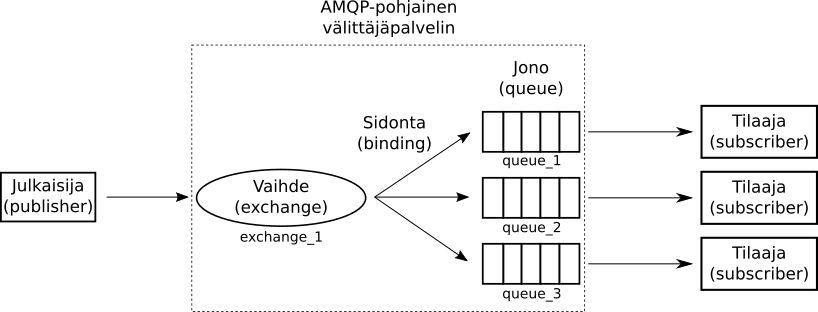
\includegraphics[width=1\textwidth]{pictures/amq-model-parts.png}
	\caption{AMQ-mallin osat ja viestin kulku niiden läpi julkaisijalta tilaajalle (pohjautuu kuvaan \cite[s.~11]{AMQP-specification}).}
	\label{fig:amq-model-parts}
\end{figure}

AMQP on ohjelmoitava protokolla siinä mielessä, että julkaisija ja tilaaja voivat määrittää komponentteja ja reitityksiä palvelimelle verkon yli ajon aikana tarpeidensa mukaan. Välittäjäpalvelin ei määritä kuin oletusvaihteet valmiiksi käytettäväksi. Toisin sanoen julkaisuja voi luoda vaihteita ja tilaaja voi luoda jonoja ja sidoksia vaihdeiden ja jonojen välille. Voidaan sanoa että julkaisija ja tilaaja tekevät uusia instansseja AMQ-mallin komponenteista palvelimelle. Vaihteiden ja jonojen instansseilla täyttyy olla välityspalvelimella yksilöivät nimet, jokainen nimi asetetaan instanssin luonnin yhteydessä. Esimerkkinä kuvassa \ref{fig:amq-model-parts} on AMQ-mallin komponenttien alla niille määritetyt nimet. Vaihteella on esimerkiksi nimi exchange\_1 ja ylimmällä jonolla queue\_1. Tällä ohjelmoitavalla ominaisuudella välityspalvelin voidaan konfiguroida toteuttamaan erilaisia skenaarioita vapaasti ja se antaa kehittäjille vapautta toteutukseen.


\subsection{Vaihde (exchange) ja reititysavain (routing-key)}
Jotta viesti voidaan välittäjäpalvelimen läpi kuljettaa, täytyy julkaisijan aloittaa määrittämällä sen käyttämä vaihde (engl. exchange) ja sen tyyppi, tai käyttää palvelimen oletusvaihdetta. Vaihde on komponentti, joka ottaa vastaan viestejä ja reitittää niitä jonoihin vaihdetyypin (engl. exchange type) ja sidosten mukaan. Vaihteet eivät ikinä tallenna viestejä. Vaihde voi tiputtaa viestin, jos se ei täsmää minkään määritetyn reitityksen kanssa. AMQ-malli määrittää seuraavat käytettävät vaihdetyypit:
\begin{itemize}
	\item suoravaihde (engl. direct exchange),
	\item hajautusvaihde (engl. fanout exchange),
	\item aihepiirivaihde (engl. topic exchange) ja
	\item otsikkovaihde (engl. header exchange).
\end{itemize}

Näitä tyyppejä ja kuinka ne toimivat käydään tarkemmin läpi tulevissa kappaleissa. Tyypin lisäksi vaihteella on myös attribuutteina nimi (engl. name), kestävyys (engl. durability), automaattinen poisto (engl. auto-delete). Nimi yksilöi vaihteen palvelimella ja tilaaja käyttää tätä nimeä sidoksen tekemiseen jonon ja vaihteen välille. AMPQ-standardissa oletetaan, että nimi on jo tiedossa etukäteen julkaisijalla ja tilaajalla. AMPQ ei tarjoa toiminnallisuutta instanssien nimien noutamiseen. Kestävyys parametrilla julkaisija voi kertoa palvelimelle, että välitäjä säilyttää vaihteen uudelleenkäynnistysten jälkeen. Jos ei, julkaisijan täytyy määrittää vaihde uudelleen käynnistyksen jälkeen. Automaattinen poisto kertoo poistaako välittäjä vaihteen automaattisesti, kun viimeinen siihen sidottu jono on poistettu ja julkaisija ei ole enää yhteydessä.

Kaikki julkaisijan ja tilaajan kutsut välittäjäpalvelimelle, jotka tekevät uuden instanssin komponentista, ovat esitteleviä (engl. declare). Tarkoittaa että palvelin tekee tarvittaessa uuden instanssin komponentista, jos sitä ei ole jo olemassa, ja vastaa samalla tavoin onnistuneesti molemmissa tapauksissa. Tilanne tulee esimerkiksi silloin kun kaksi julkaisijaa käyttävät samaa vaihdetta keskenään. Toinen ei tiedä onko toinen jo määrittänyt instanssin vaihteesta palvelimelle, esimerkiksi silloin kun ohjelmat käynnistyvät eri aikaan. Jos kummatkin julkaisijat eksplisiittisesti määrittävät saman käytettävän vaihteen. Palvelin vastaa kummallekin onnistuneesti ja tuloksena palvelimella on vain yksi instanssi halutusta vaihteesta. Sama toiminta pätee kaikkiin välittäjäpalvelimen kutsuihin, jotka tekevät uusia instansseja komponenteista.

Vaihde reitittää viestejä jonoihin sen sidosten ja tyypin mukaan. Kuitenkin reititykseen liittyy yksi tärkeä asia kuin reititysavain (engl. routing-key). Reititysavain on kuin virtuaalinen osoite viestissä, jonka julkaisija liittää viestiin julkaisun yhteydessä. Tilaaja käyttää myös reititysavainta jonon määrityksen yhteydessä. Vaihde, tyypistä riippuen, voi käyttää tätä avainta reititykseen eri jonoihin. Viestin reititysavainta voi hyvin verrata lähetettävän sähköpostin saaja-kenttään. Saaja kertoo vastaanottajan sähköpostiosoitteen, johon viesti on tarkoitus lähettää. Reititysavain toimii juurikin näin suorassa viestin lähetyksessä, mutta eroaa muissa.


\subsection{Suoravaihde (direct exchange)}
Julkaisija voi määrittää vaihteen instanssin tyypiksi suoravaihteen (engl. direct exchange). Suoravaihde reitittää viestin jonoihoin suoraan vastaavan reititysavaimen perusteella. Suoravaihde reitittää seuraavasti:
\begin{itemize}
	\item tilaaja määrittää sidoksen reititysavaimella K,
	\item julkaisija julkaisee viestin reititysavaimella R,
	\item vaihde välittää viestin jonoon jos K = R,
	\item muuten vaihde tiputtaa tai palauttaa viestin lähettäjälle.
\end{itemize}
Kuvassa \ref{fig:amqp-direct-exchange} on esitetty suoravaihteen toiminta. Vaihteeseen on tehty sidoksia reititysavaimilla \emph{error} ja \emph{info}. Yksi tilaaja voi luoda sidoksia samaan vaihteeseen monella eri reititysavaimella. Näin tilaaja voi tilata viestejä mistä on kiinnostunut. Kuvassa \ref{fig:amqp-direct-exchange} julkaisija julkaisee viestin reititysavaimella info. Viesti päätyy molempiin queue\_1 ja queue\_2 jonoon. Reititysavaimella error, viestit päätyvät vain jonoon queue\_1. Välittäjäpalvelin tarjoaa suoravaihteesta oleutusvaihteen nimeltä amq.direct. \cite[s.~27]{AMQP-specification}

\begin{figure}[ht!]
	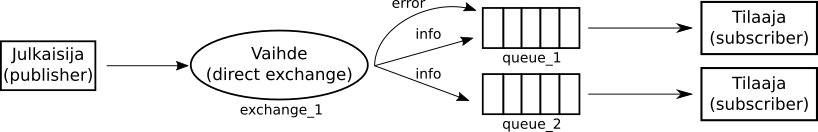
\includegraphics[width=1\textwidth]{pictures/amqp-direct-exchange.png}
	\caption{Suoravaihde (engl. direct exchange), reitittää suoraan sidoksen reititysavaimen mukaan (pohjautuu kuvaan \cite{RabbitMQ-Tutorial-Routing}).}
	\label{fig:amqp-direct-exchange}
\end{figure}


\subsection{Hajautusvaihde (fanout exchange)}
Julkaisija voi määrittää vaihteen instanssiksi hajautusvaihteen (engl. fanout exchange). Hajatusvaihde reitittää viestit kaikkiin sen jonoihin reititysavaimesta välittämättä. Hajautusvaihde toimii seuraavasti:
\begin{itemize}
	\item tilaaja määrittää sidoksen vaihteeseen reititysavaimella K,
	\item julkaisija julkaisee viestin reititysavaimella R,
	\item vaihde välittää viestin kaikkiin siihen sidottuihin jonoihin, reititysavaimesta riippumatta.
\end{itemize}
Kuvassa \ref{fig:amqp-fanout-exchange} on esitetty hajautusvaihteen toiminta. Vaihteeseen exchange\_1 on tehty kolme eri sidosta jonoihin queue\_1, queue\_2 ja queue\_3. Julkaisijan lähettämä viesti lähetetään kaikkiin kolmeen sidottuun jonoon, viestin ja jonojen reititysavaimista riippumatta. Välittäjäpalvelin tarjoaa hajautusvaihteesta oletusvaihteen nimeltä amq.fanout. \cite[s.~27]{AMQP-specification}

\begin{figure}[ht!]
	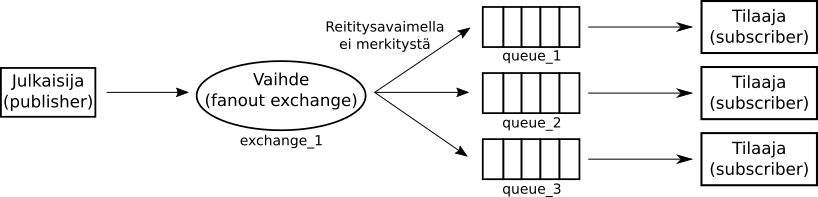
\includegraphics[width=1\textwidth]{pictures/amqp-fanout-exchange.png}
	\caption{Hajautusvaihde (engl. fanout exchange) reitittää kaikkiin siihen sidottuihin jonoihin riippumatta reititysavaimesta (pohjautuu kuvaan \cite{RabbitMQ-AMQP-0-9-1-Model-Explained}).}
	\label{fig:amqp-fanout-exchange}
\end{figure}


\subsection{Aihepiirivaihde (topic exchange)}
Aihepiiri vaihdetyyppi (engl. topic exchange) reitittää viestejä sidottuihin jonoihin reititysavaimen mukaan, kuten suoravaihde, mutta tarjoaa lisäksi sääntöjä monen avaimen samanaikaiseen yhteensopivuuteen. Sidoksen reititysavaimen sijaan voidaan puhua reitityskaavasta (engl. routing pattern). Aihepiiri vaihde toimii seuraavasti:
\begin{itemize}
	\item tilaaja määrittää sidoksen vaihteeseen reitityskaavalla P,
	\item julkaisija julkaisee viestin reititysavaimella R,
	\item vaihde välittää viestin jonoon, jos sen reitityskaava P sopii reititysavaimeen R.
\end{itemize}
Aihepiirivaihteen yhteydessä AMQP-standardi määrittää että viestin reititysavain täytyy olla lista sanoja jotka ovat erotettu pisteillä ja ovat yhdessä maksimissaan 255 merkkiä pitkä \cite[s.~35]{AMQP-specification}. Sanat saavat sisältää kirjaimia A-Z ja a-z, ja numeroita 0-9. Yleensä avaimeen sijoitetaan sanoja mitkä liittyvät viestin sisältöön. Tilaajan määrittämä sidoksen reitityskaava voi olla samaa muotoa kuin reititysavain, mutta sanojen tilalla voidaan käyttää seuraavia erikoismerkkejä:
\begin{itemize}
	\item \textbf{*} (tähti), voi vastata mitä tahansa yhtä sanaa,
	\item \textbf{\#} (risuaita), voi vastata nolla tai monta sanaa. \cite[s.~27]{AMQP-specification}
\end{itemize}

Kuvassa \ref{fig:amqp-topic-exchange} on esitetty aihepiirivaihteen toiminta. Vaihteeseen exchange\_1 on sidottu jono queue\_1 reitityskaavoilla \textbf{app1.\#} ja \textbf{*.*.warn}. Ja jono queue\_2 reitityskaavalla \textbf{*.log.*}. Oletetaan että julkaisija lähettää viestejä avaimella muodossa \emph{ohjelma.kanava.taso}, jossa sana ohjelma kuvaa julkaisijan nimeä. Kanava, kuvaa lokitusväylää ja taso kuvaa viestin tasoa (warning, error, info jne.). Voisi sanoa että queue\_1 on kiinnostunut kaikista ohjelmalta app1 tulevista viesteistä ja myös kaikista varoitustason (warning) viesteistä kaikilta ohjelmilta. Jono queue\_2 on taas kiinnostunut kaikista log-väylän viesteistä.

\begin{figure}[ht!]
	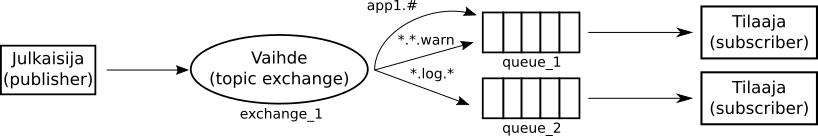
\includegraphics[width=1\textwidth]{pictures/amqp-topic-exchange.png}
	\caption{Aihepiirivaihde (engl. topic exchange), reitittää kaikkiin siihen sidottuihin jonoihin, joiden reitityskaava sopii viestin reititysavaimeen (pohjautuu kuvaan \cite{RabbitMQ-Tutorial-Topics}).}
	\label{fig:amqp-topic-exchange}
\end{figure}

Nyt jos julkaisija lähettää viestin avaimella \textbf{app1.debug.warn}. Vaihde välittää viestin jonoon queue\_1, mutta ei jonoon queue\_2. Avaimella \textbf{app2.log.info} viesti välitetään vain jonoon queue\_2. Avaimella \textbf{app1.log.warn} viesti lähetään molempiin jonoihin. Kun taas avaimella \textbf{app2.debug.info} viestiä ei lähetetä yhteenkään jonoon.

Aihepiirivaihde on vaihdetyypeistä monimutkaisin, mutta kattaa ison määrän erilaisia käyttötapauksia. Vaihteen avulla tilaajat voivat tilata viestejä, joista ovat esimerkiksi kiinnostuneita. Aihepiirivaihdetta voi käyttää kuin aikaisempia vaihdetyyppejä. Jos jono sidotaan reitityskaavalla \textbf{\#}, se vastaanottaa kaikki viestit kyseiseltä vaihteelta ja käyttäytyy kuin hajautusvaihde. Jos jono sidotaan ilman merkkejä \textbf{*} ja \textbf{\#}, niin se käyttäytyy samalla tavalla kuin suoravaihde. \cite{RabbitMQ-Tutorial-Topics}


\subsection{Otsikkovaihde (headers exchange)}
Otsikkovaihde (engl. headers exchange) on vaihdetyyppi joka ei käytä reititysavainta ollenkaan reititykseen, vaan reititys perustuu viestin ja sidoksen otsikkotietoihin. Otsikkotiedot koostuvat avain--arvo-pareista. Otsikkovaihde toimii seuraavasti:
\begin{itemize}
	\item tilaaja määrittää sidoksen vaihteeseen otsikkotiedoilla H,
	\item julkaisija julkaisee viestin otsikkotiedoilla O,
	\item vaihe välittää viestin jonoon jos otsikkotiedot O vastaavat otsikkotietoja H, riippuen sidoksen otsikkotiedoissa olevasta \textbf{x-match} kentän arvosta.
\end{itemize}
Jonon sidoksen määrityksen yhteydessä tilaaja voi asettaa kentän \textbf{x-match} otsikkotietoihin ja sille arvon kahdesta eri mahdollisuudesta \textbf{all} tai \textbf{any}. Arvot toimivat seuraavasti:
\begin{itemize}
	\item \textbf{all} kertoo vaihteelle, että jokainen viestin otsikkotieto täytyy vastata sidoksen otsikkotietoja (boolen algebrassa AND-operaatio), jotta viestin lähetetään jonoon,
	\item \textbf{any} kertoo vaihteelle, että mikä vain viestin otsikkotiedoista löytyy sidoksen otsikkotiedoista (boolen algebrassa OR-operaatio), lähetetään viesti jonoon. \cite[s.~28]{AMQP-specification}
\end{itemize}

Otsikkotiedoissa arvot ovat vaihtoehtoisia asettaa. Jos kentän arvoa ei ole asetettu, vastaavuus on kun kentän nimet ovat samat. Jos kentän arvo on asetettu, vastaavuus on jos molemmat nimi ja arvo vastaavat toisiaan. \cite[s.~28]{AMQP-specification}


\subsection{Jonon määritys ja viestien kuittaaminen}
AMQ-mallissa jono (engl. queue) on vaihteen ja tilaajan välissä oleva puskuri (kuva \ref{fig:amq-model-parts}), joka tallentaa tilaajalle tulevia viestejä. Jono pitää viestejä jonossa tilaajalle, kunnes tämä ehtii prosessoida ne. Yksi jono voi puskuroida viestejä monelle eri tilaajalle. Tilaaja sitoo (engl. binding) jonon nimellä johonkin palvelimella jo olevaan vaihteeseen mistä viestejä haluaa. Tilaajan täytyy tietää vaihteen nimi. Jonolla tilaaja voi määrittää attribuutteja. Jotkin attribuutit ovat samoja kuin vaihteella. Tilaaja voi määrittää jonolle nimen (engl. name), kestävyyden (engl. durable), poissulkevuuden (engl. exclusive) ja automaattisen poiston (auto-delete). Nimi yksilöi jonon palvelimella. Tilaaja voi halutessaan pyytää palvelinta generoimaan yksilöivän nimen jonolle automaattisesti. Kestävyys-attribuutti säilyttää jonon palvelimella uudelleenkäynnistyksen jälkeen. Poissulkeva rajoittaa jonon vain yhdelle tilaajalle ja palvelin poistaa jonon kun yhteys tilaajaan katkeaa. Automaattinen poisto poistaa jonon palvelimelta automaattisesti kun yhteys viimeiseen tilaajan on katkennut. \cite{RabbitMQ-AMQP-0-9-1-Model-Explained}

Jono lähettää viestin vain yhdelle jonossa olevalle tilaajalle. Sama viesti lähetetään ainoastaan toiselle tilaajalle jos se edelleenlähetetään virheen tai peruutuksen seurauksena. Jos samassa jonossa on monta eri tilaajaja, jono lähettää viestejä monelle tilaajalle kiertovuorottelun (engl. round-robin) periaatteen mukaan. \cite[s.~11--12]{AMQP-specification}

Tilaajan täytyy määrittä jonolle sen käyttämä viestin kuittaamisen (engl. acknowledge) malli ennen kuin jono poistaa viestin puskurista. Malleja on kaksi:
\begin{itemize}
	\item automaattinen, jolloin palvelin poistaa viestin jonosta heti kun se on lähetetty tilaajalle,
	\item eksplisiittinen, jolloin palvelin poistaa viestin vasta kun tilaaja on lähettänyt kuittauksen palvelimelle.
\end{itemize}
Tilaaja voi lähettää viestistä kuittauksen milloin vain prosessoinnin aikana. Heti kun viesti on vastaanotettu tai silloin kun viesti on prosessoitu. \cite[s.~29]{AMQP-specification}
\chapter{Projektin lähtökohdat}
\label{ch:projektin-lähtökohdat}
Tarkoituksena tässä diplomityössä oli toteuttaa ohjelmistokomponentti osaksi isompaa järjestelmää. Isompi järjestelmä liittyi sähköasemien toimintaan ja niiden tarkkailuun. Ohjemistokomponentin tarkoituksena oli tilata viestejä sähköaseman IED-laitteen RCB-instansseilta IEC 61850 -standardin mukaisesti. Standardin mukainen viesti prosessoitiin ja jaettiin järjestelmän muiden komponenttien kanssa. Esimerkiksi viesti voi sisältää mittaustietoa, joka halutaan näyttää loppukäyttäjälle käyttöliittymässä. Käyttöliittymän päivittävä komponentti tarvitsee mittaustiedon IED-laitteelta.

Ennen tämän työn aloittamista yrityksessä oli jo kehitetty ensimmäinen versio ohjelmasta. Ohjelma kykeni tilaamaan viestejä IED-laitteen kaikilta RCB-instansseilta, prosessoimaan viestit ja tallentamaan ne relaatiotietokantaan myöhempää käyttöä varten. Tässä ohjelmistossa oli havaittuja ongelmia ja se ei myöskään tukenut kaikkia IEC 61850 -standardin viesteihin liittyviä ominaisuuksia. Tämän ohjelmiston toimintaperiaate ja siinä olleet ongelmat toimivat pohjana uuden version suunnittelulle ja toteutukselle. Tarkoituksena oli poistaa havaitut ongelmakohdat ja miettiä olisiko jokin muu arkkitehtuuri parempi kyseiseen toteutukseen. Ensimmäistä toteutusta ohjelmasta voisi nimittää ensimmäiseksi protoversioksi tai demovaiheeksi (engl. proof of concept), jonka pohjalta tultiin tekemään toimiva lopullinen versio. Tekstissä eteenpäin sanoilla demo ja demoversio viitataan tähän ohjelmistoon.

Tässä osiossa pohjustetaan työn alkua lukijalle ja mistä lähdettiin liikkeelle. Lisäksi kuvataan mitä ongelmia demovaiheen toteutuksessa ja oli ja analysoidaa niitä. Demovaiheen ohjelmasta käsitellään sen arkkitehtuuria, mitkä olivat sen komponentit ja niiden toiminnallisuus. Tässä käsitellyt ongelmat toimivat pohjana uuden version suunnittelulle ja auttavat tekemään siihen liittyviä ratkaisuja.


\section{Demon arkkitehtuuri}
\label{ch:demoversio-ja-sen-toiminta}
Demoversio oli ohjelmoitu Ruby-ohjelmointikielellä. Ohjelman arkkitehtuuri oli yksinkertainen. Kuvassa \ref{fig:demo-architecture} on esitetty demoversion arkkitehtuuri korkealla tasolla ja kuinka viesti IED-laitteelta kulkee tietokantaa. Yksi ajettu demoversion prosessi pystyi tilaamaan yhden IED-laitteen kaikki RCB-luok\-ki\-en instanssit. Instanssien tiedot luettiin relaatiotietokannasta. Ohjelmisto prosessoi viestit ja tallentamaan ne relaatiotietokantaan myöhempää käyttöä varten. Ruby-ohjelmistossa tärkeässä osassa oli \emph{libIEC61850}-kirjasto \cite{libIEC61850-homepage}. libIEC61850-kirjasto on avoimen lähdekoodin C-kielellä toteutettu kirjasto, joka abstrahoi IEC 61850 -standardin matalan tason määrittämiä palvelukutsuja ja datarakenteita helppokäyttöiseksi rajapinnaksi. Kirjasto tarjosi toiminnallisuuden IED-laitteella olevan palvelinohjelmiston, sekä IED-laittetta käyttävän asiakaohjelmiston toteuttamiseen. IED-laitteen palvelimelle kirjasto tarjosi funktioita ja rakenteita IEC 61850 määrittämien luokkien ja hierarkian rakentamiseen ja käsittelyyn. IED-laitteen asiakasohjelmalle kirjasto tarjosi funktioita ja rakenteita standardin määrittämiin palveluihin, kuten arvojen lukuun ja asettamiseen, datajoukkojen käyttöön ja viestien tilaamiseen. Tätä samaa kirjastoa käytettiin myös tässä työssä toteutetussa ohjelmistokomponentissa. Demossa ja lopullisessa ohjelmistokomponentissa käytettiin vain kirjaston tarjoamia IED-laitteen asiakasohjelmiston ominaisuuksia

\begin{figure}[ht!]
	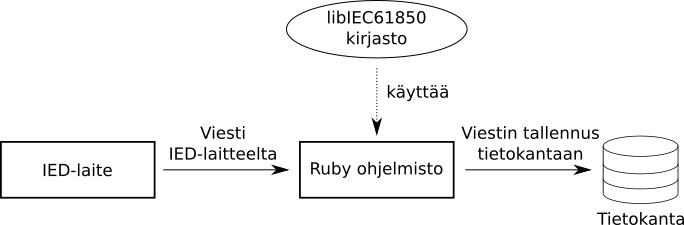
\includegraphics[width=1\textwidth]{pictures/demo-architecture.png}
	\caption{Rubylla toteutetun demoversion arkkitehtuuri ja tiedonsiirto.}
	\label{fig:demo-architecture}
\end{figure}

LibIEC61850-kirjasto on rakennettu käyttämään MMS-protokollaa tiedonsiirrossa IED-laitteen ja sen asiakasohjelman välillä, kuten IEC 61850 -standardin osassa 8-1 määritetään. Kuvassa \ref{fig:libiec61850-layer-architecture} on esitetty kirjaston kerrosarkkitehtuuri asiakasohjelmalle. Kirjastoon on toteutettu \emph{laiteabstraktiokerros} (engl. \emph{Hardware Abstraction Layer}, lyhennetään \emph{HAL}). HAL:in avulla kirjasto voi toimia monella eri laitealustalla, ja käyttäjä voi tarvittaessa lisätä oman HAL-implementaation. Demoversiota suoritettiin Linux-käyttöjärjestelmällä, joten kirjastosta käytettiin olemassa olevaa Linux HAL -toteutusta. Kuvassa \ref{fig:libiec61850-layer-architecture} on punaisella merkitty laatikot, jotka kirjaston käyttäjä voi tarjota itse, keltaisella kirjaston uudelleenkäytettävät MMS-protokollan osuudet ja sinisellä IEC 61850 -standardin toteuttavat osuudet. Kuvaan on merkitty vihreällä demoon toteutetut osuudet, eli Ruby-kielelle liitos C-kieleen ja tämän päälle Rubylla tehty ohjelmisto.

\begin{figure}[ht!]
	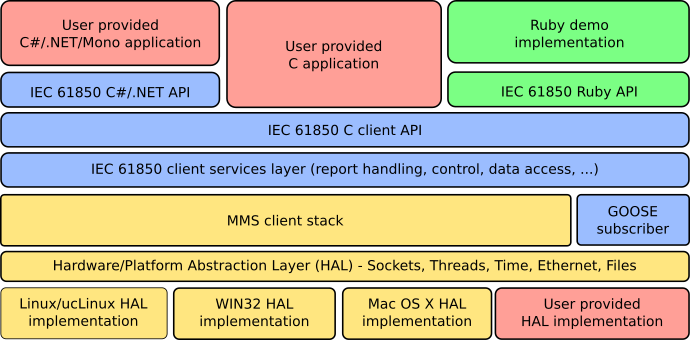
\includegraphics[width=1\textwidth]{pictures/libiec61850-layer-architecture.png}
	\caption{libIEC61850-kirjaston kerrosarkkitehtuurin komponentit, vihreällä Ruby toteutukseen lisätyt osat (pohjautuu kuvaan \mbox{\cite{libIEC61850-api-overview}}).}
	\label{fig:libiec61850-layer-architecture}
\end{figure}

Ruby-koodista C-kielen funktioiden kutsuminen ei ole suoraan mahdollista, vaan kielten väliin täytyy toteuttaa liitos. Demoversiossa liitos oli tehty käyttäen Rubylle saatavaa \emph{ruby-ffi} -kirjastoa \cite{ruby-ffi-repo} (engl. \emph{Foreign Function Interface}, lyhennetään \emph{FFI}). Liitoksen avulla Ruby voi kutsua C-kielen funktioita ja käyttää sen struktuureita ja muuttujia. Demossa kirjasto huolehti matalan tason IEC 61850 asiat, ja Ruby-koodi keskittyi liitoksen avulla korkean tason viestin jäsentämiseen ja tallennukseen tietokantaan.


\section{Demon toiminta ja sen ongelmat}
\label{ch:ongelmakohdat-ja-analysointi}
Demo oli toteutettu käyttäen \emph{Ruby on Rails} -kehystä, lyhennetään \emph{RoR}. RoR on tarkoitettu web-sovellusten toteuttamiseen Ruby-kielellä. Se tarjoaa \emph{Active Record} nimisen \emph{ORM}-kerroksen (engl. \emph{Object-Relational Mapping}) tietokannan käsittelyn helpottamiseen. ORM-kerros abstrahoi relaatiotietokannan käyttämisen oliopohjaiseksi ja kyselyitä tietokantaan voi tehdä suoraan Ruby-kielellä. Demo käytti RoR:in ORM-kerrosta tietokannan käyttämiseen. Demossa päädyttiin käyttämään RoR-kehystä, koska muu järjestelmä oli toteutettu tällä kehyksellä. Ennen suorittamista ohjelmaan täytyi ladata RoR:in ympäristö muistiin, jonka seurauksena yksinkertaisen ohjelman piti varata iso määrä muistia.

Ohjelman toiminta on esitetty sekvenssikaavioissa \ref{fig:sequence-diagram-report-subscription} ja \ref{fig:sequence-diagram-report-subscription-processing}. Sekvenssikaavio \ref{fig:sequence-diagram-report-subscription} jatkuu kuvassa \ref{fig:sequence-diagram-report-subscription-processing}. Kuvissa ohjelman kaksi eri silmukkaa on esitetty loop-laatikoilla. Sekvenssikaaviossa osallisena ovat tietokanta, Ruby-ohjelma, libIEC61850-kirjasto, libIEC61850-kirjaston natiivisäie ja IED-laiteen palvelinohjelma. Rubyn ja libIEC61850-kirjaston liitos oli tehty ruby-ffi -kirjastolla ja kirjaston natiivisäie on vastuussa yhteyden ylläpidosta ja datan siirtämisestä. Sekvenssikaavioon on merkitty paksulla suorituksessa olevat palkit, esimerkiksi IED-laitteen palvelinohjelmisto on koko ajan suorituksessa. Tulevassa tekstissä viitataan molempien kuvien kohtiin numeroilla.

\begin{figure}[ht!]
	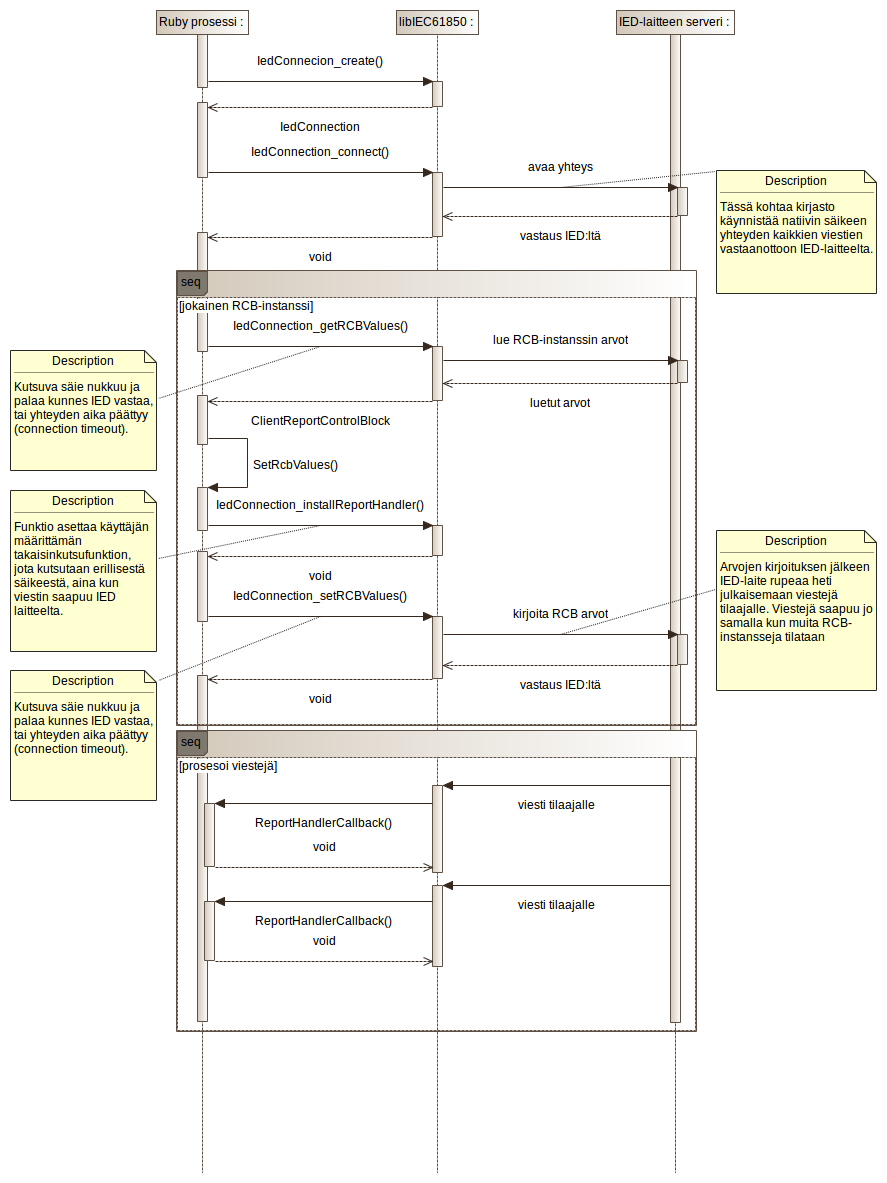
\includegraphics[width=1\textwidth]{pictures/sequence-diagram-report-subscription.png}
	\caption{Sekvenssikaavio kuinka Ruby-ohjelma avaa yhteydet ja tilaa kaikki IED-laitteen RCB-instanssit (jatkuu kuvassa \ref{fig:sequence-diagram-report-subscription-processing}).}
	\label{fig:sequence-diagram-report-subscription}
\end{figure}

\begin{figure}[ht!]
	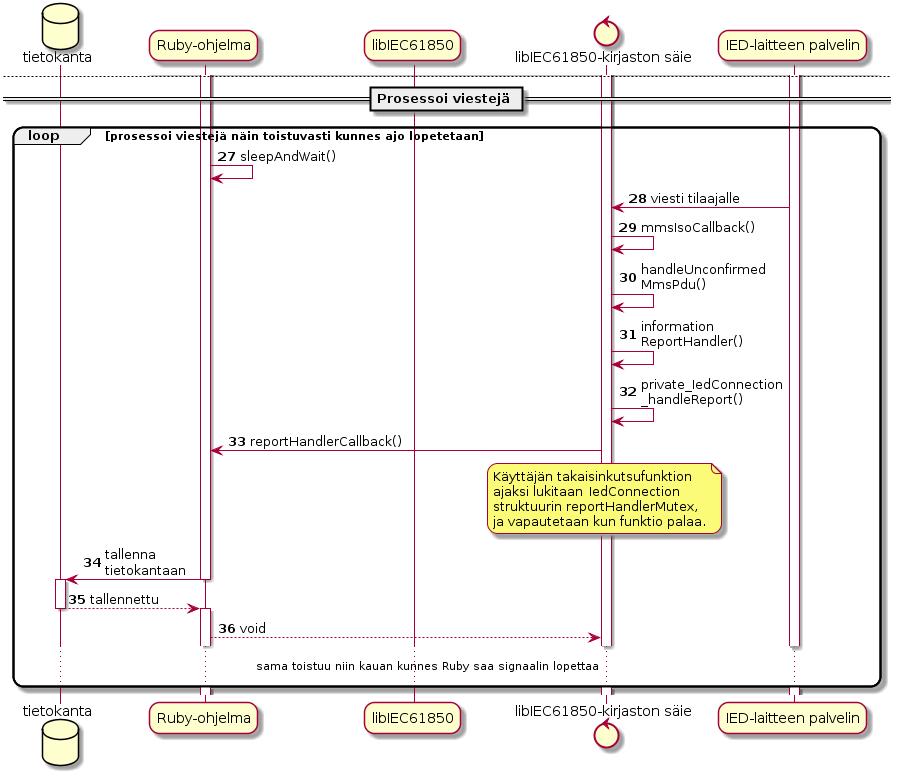
\includegraphics[width=1\textwidth]{pictures/sequence-diagram-report-subscription_001.png}
	\caption{Sekvenssikaavio kuinka Ruby-ohjelma prosessoi ja tallentaa viestejä libIEC61850-kirjastoa käyttäen (jatkuu kuvasta \ref{fig:sequence-diagram-report-subscription}).}
	\label{fig:sequence-diagram-report-subscription-processing}
\end{figure}

Ensimmäisenä ohjelma luki tietokannasta IED-laitteen, sekä sen kaikki RCB-instanssien tiedot. Tämän avulla ohjelma tiesi mikä IED-laitteen IP-osoite on ja mitkä olivat RCB-instanssien viitteet (kohdat 1--2). Ohjelmaan pystyi syöttämään eri tietoja ainoastaan tietokannan kautta ennen suoritusta. Tämän jälkeen ohjelma pystyi muodostamaan yhteyden IED-laitteelle tekemällä instanssin \texttt{IedCon\-nec\-ti\-on} struktuurista funktiolla \texttt{Ied\-Con\-nec\-ti\-on\_crea\-te\-()} (kohdat 3--4). Tämän jälkeen struktuuri annetaan \texttt{Ied\-Con\-nec\-ti\-on\-\_\-con\-nect\-()} funktiolle, joka avaa yhteyden IED-laitteelle ja palaa vasta kun vastaus saapuu (kohdat 5--11). Tässä vaiheessa libIEC61850-kirjasto käynnistää erillisen natiivisäikeen yhteyden viestien vastaanottoon. Tätä säiettä kirjasto käyttää tulevien viestien vastaanottoon ja lähettämiseen. Yhteyden avauksen jälkeen jokainen RCB-instanssi tilataan lukemalla ensin sen arvot IED-laitteelta funktiolla \texttt{Ied\-Con\-nec\-ti\-on\-\_\-get\-RCB\-Va\-lu\-es\-()} (kohta 12). Funktiokutsu nukkuu ja palaa vasta kunnes erillinen säie ilmoittaa että vastaus on saapunut, tai yhteyden aika ylittyy. Kirjaston funktio  \texttt{send\-Re\-qu\-est\-And\-Wait\-For\-Res\-pon\-se\-()} nukkuu ja odottaa vastausta (kohdat 13--16). RCB-arvot luettuaan, kirjasto palauttaa struktuurin \texttt{Cli\-ent\-Re\-port\-Cont\-rol\-Block}, joka sisältää luetut tiedot RCB-instanssista (kohta 17). Samaa struktuuria käytetään arvojen muuttamiseen ja niiden takaisin kirjoittamiseen IED-laitteelle. Ennen muunneltujen RCB-arvojen takaisin kirjoittamista ja viestien tilaamista, täytyy kirjastolle asettaa takaisinkutsufunktio, jota kirjasto kutsuu aina kun tilattu viesti saapuu IED-laitteelta. Takaisinkutsufunktioksi asetetaan funktiolla \texttt{Ied\-Con\-nec\-ti\-on\-\_\-ins\-tall\-Re\-port\-Hand\-ler\-()} (kohdat 19--20). Asetuksen ajaksi kirjasto lukitsee \texttt{re\-port\-Hand\-ler\-Mu\-tex}:in. Tätä samaa lukitusta käytetään kun viesti takaisinkutsufunktiota kutsutaan viestin saapuessa (kohdat 33--36). Tilanteessa jossa takaisinkutsufunktiota asetetaan samalla kun viesti on saapunut, joutuu toinen osapuoli odottamaan lukituksen vapautumista. Tämä lukitus on tärkeä huomio myöhemmin kun käydään läpi ohjelman huonoa suorituskykyä. Tämän jälkeen arvot kirjoitetaan takaisin IED-laitteelle funktiolla \texttt{Ied\-Con\-nec\-ti\-on\-\_\-set\-RCB\-Va\-lu\-es\-()} (kohdat 21--26). Tämä funktio palaa vasta kun IED vastaa tai yhteyden aika ylittyy. Heti arvojen kirjoitusten jälkeen IED aloittaa lähettämään viestejä tilaajalle. Eli samalla kun muita RCB-instansseja tilataan, tilatut RCB-instanssit lähettävät jo viestejä ja aiheuttavat takaisinkutsufunktion suorittamisen. Kun kaikki RCB-instanssit on tilattu, ohjelma jää viimeiseen silmukkaan odottamaan ja prosessoimaan viestejä (kohdat 27--36). Kun viesti saapuu, säie kutsuu ensin sisäisesti \texttt{mms\-I\-so\-Call\-back\-()} funktiota, joka kutsuu muita kirjaston sisäisiä funktioita ja lopuksi asetettua takaisinkutsufunktiota (kohdat 28--33). Takaisinkutsufunktio on liitetty Ruby funktioon ja funktio tallentaa raportin tiedot tietokantaan (kohdat 33--36). Ruby-funktion suorituksen ajaksi kirjasto lukitsee \texttt{re\-port\-Hand\-ler\-Mu\-tex}:in, ja vapautetaan kunnes Ruby-funktion suoritus palaa. Tätä jatkuu niin kauan kun ohjelmalle lähetetään jokin signaali joka lopettaa sen suorituksen. \mbox{\cite{Kozlovski2017, Storimer2013, libIEC61850-repo}}

Demossa isoimpana ongelmana oli sen huono suorituskyky ja toiminnan epävarmuus RCB-instanssien määrän ollessa enemmän kuin muutama. RCB-instanssien määrän ollessa liian suuri ohjelma saattoi epäonnistui joidenkin tilaamisessa, koska yhteys aikakatkaistiin arvojen kirjoituksessa tai luvussa. Lisäksi ongelmaksi muodostui usean RCB instanssin tilaamisen kulunut aika. Yhteensä aikaa saattoi kulua 30 sekuntia kaikkien instanssien tilaamiseen.

Huonoon suorituskykyyn oli syynä muutama asiaa. Yksi niistä oli Ruby-kielen huonompi suorituskyky verrattuna natiivisti käännettyyn C-kieleen. Ruby on tulkattava kieli kuten esimerkiksi Python, joka tulkataan rivi kerrallaan ja suoritetaan. Lähdekoodia ei käännetä kokonaan ensin konekäskyiksi erillisellä kääntäjällä, kuten C-kielessä. Valmiiksi käännetty lähdekoodi tarvitsee vain ajaa, kun taas tulkattavassa kielessä rivi täytyy ensin tulkata ja sitten ajaa. Rubyssa käytettiin sen oletustulkkia \emph{MRI/YARV} (engl. \emph{Matz's Ruby Interpreter}, lyhennetään \emph{MRI} tai \emph{Yet another Ruby VM}, lyhennetään \emph{YARV}). Ruby versiosta 1.9 eteenpäin käyttää YARV-tulkkia. Toinen syy oli Ruby-kielen oletustulkissa oleva \emph{globaali tulkkilukitus} (engl. \emph{Global Interpreter Lock}, lyhennetään \emph{GIL}, tai \emph{Global Virtual Machine Lock}, lyhennetään \emph{GVL}). GIL pakottaa Ruby-ohjelman ajoon vain yhdellä ytimellä ja vain yksi säie vuorossa kerrallaan ja on täysin riippumaton käyttöjärjestelmän vuorottajasta \mbox{\cite[s.~131--133]{Odaira2014}}. Kuvassa \ref{fig:ruby-gil} on esitetty kuinka Ruby-tulkki vuorottaa kahta ajossa olevaa säiettä. Kuvassa demon Ruby-koodi kutsuu \texttt{Ied\-Con\-nec\-ti\-on\-\_\-set\-RCB\-Va\-lu\-es\-()} funktiota, ajo jää kesken ja tapahtuu vaihto, koska viesti saapui. Takaisinkutsufunktio suoritetaan ja suoritus palaa takaisin aikaisempaan funktion suoritukseen. Tässä vaiheessa jos vaihto on huonolla hetkellä ja kesti liian kauan, tulee yhteyden aikakatkaisu ja RCB-instanssi jää tilaamatta. Huonoon suorituskykyyn mahdollisesti vaikutti myös lukitus \texttt{re\-port\-Hand\-ler\-Mu\-tex} jota kirjastossa käytetään kun takaisinkutsufunktio asetetaan ja takaisinkutsufunktio suoritetaan. Lukitus aiheuttaa säikeen nukkumisen niin kauan kun lukitus vapautuu. Tässä tapauksessa jos viestin prosessointi kestää kauan (kuvassa \ref{fig:sequence-diagram-report-subscription-processing} kohdat 33--36) ja vielä muita RCB-instansseja tilataan silmukassa (kuvassa \ref{fig:sequence-diagram-report-subscription} kohdat 12--26). Säie joutuu odottamaan lukituksen vapautusta kun takaisinkutsufunktioita asetetaan (kohdat 19--20). Ratkaisuna tähän olisi pitää takaisinkutsufunktio mahdollisimman lyhyenä suoritusajan suhteen.

\begin{figure}[ht!]
	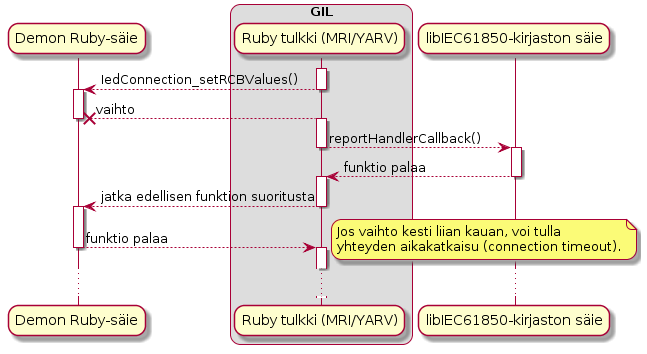
\includegraphics[width=1\textwidth]{pictures/ruby-gil.png}
	\caption{Ruby-tulkin globaalin lukituksen toiminta, joka vuorottaa ajossa olevia säikeitä riippumatta käyttöjärjestelmän vuorottajasta.}
	\label{fig:ruby-gil}
\end{figure}

Tämän lisäksi demototeutuksessa oli muistivuoto. Muistivuoto on tilanne missä ohjelma varaa kokoajan lisää muistia ja ei vapauta sitä takaisin käyttöjärjestelmälle uudelleen käyttöön. Muistivuoto johtui todennäköisesti jostakin ohjelmointivirheestä ruby-ffi -kirjaston liitoksen kanssa. Kun liitos Rubysta tehdään C-kieleen, täytyy ohjelmoijan miettiä roskien keruuta tarkasti. Tätä ei normaalisti tarvitse miettiä Rubyssä, koska tulkki implementoi automaattisen roskien keruun. Muistivuoto havaittiin kun ohjelma jätettiin suoritukseen pitemmäksi aikaa ja ohjelma oli varannut melkein kaiken käyttöjärjestelmän muistista itselleen. Lisäki jos ohjelmaa ajaa ja tarkkailee Linuxin \emph{htop}-ohjelmalla, voi \emph{MEM\%}-sarakkeesta huomata prosentuaalisen osuuden kasvavan koko käyttöjärjestelmän muistista.

Näiden lisäksi tiedon jako järjestelmän muiden komponenttien kanssa oli huono. Ohjelma prosessoi viestit relaatietokantaan. Muiden komponenttien täytyi kysellä tietoa tietokannasta tasaisin väliajoin, ilman tietoa milloin uusi tieto on saatavissa. Komponenttien määrästä riippuen tietokanta on turhan rasituksen alaisena jatkuvasti. Tulevaisuutta ajatellen lopullinen tiedon tallennuspaikka ei ole muiden tietoa tarvitsevien ohjelmien kannalta järkevä. Tarvittaisiin keino, jolla komponentit voisivat saada tiedon uudesta viestistä erikseen, ilman että sitä täytyisi kysellä väliajoin.
\chapter{Suunnittelu}
\label{ch:suunnittelu}
\begin{it}
	Pitäisikö tähän kirjoittaa ohjelman ajosta ja siihen liittää sekvenssikaavio perustoimminnasta? Kirjoita jos tuntuu että tarvetta.
\end{it}
Tässä osuudessa käydään toteutetun ohjelman suunnittelu läpi ja kerrotaan miten ja miksi ratkaisuihin päädyttiin. Kappaleissa vertaillaan eri vaihtoehtoja ja peilataan demoversion ongelmia ja niiden perusteella yritetään löytää toimiva ratkaisu ongelmaan. Ensin suunnitellusta ohjelmasta annetaan kattava kokonaiskuva lukijalle ja tämän jälkeen tulevissa kappaleissa mennään jokaisen kohdan yksityiskohtiin tarkemmin.


\section{Kokonaiskuva}
Aikaisemmin kappaleessa \ref{ch:demoversio-ja-sen-toiminta} kuvassa \ref{fig:demo-architecture} esiteltiin demoversion arkkitehtuuri ja sen toiminta. Kuinka viestit IED-laitteelta kulkee ohjelman läpi ja tallennetaan tietokantaan. Tietokannasta muut ohjelmat lukevat tietoa kyselemällä sitä erikseen. Suunnittelun jälkeen demoversion järjestelmästä päätyttiin kuvassa \ref{fig:planned-system-architecture} olevaan järjestelmän arkkitehtuuriin. Kuvassa katkoviivalla on merkitty tässä kappaleessa suunniteltu ohjelmisto. Ja kuvan yläreunassa oleva viiva kuvaa viestin kulkua järjestelmän eri osapuolten läpi ja missä muodossa viesti on missäkin kohtaa.

\begin{figure}[ht!]
	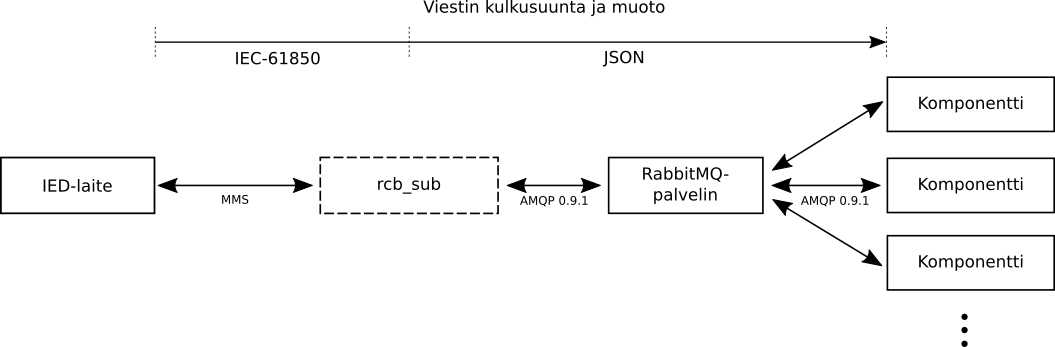
\includegraphics[width=1\textwidth]{pictures/planned-system-architecture.png}
	\caption{Suunnitellun järjestelmän toiminta ja viestin kulkeminen ja muoto eri osapuolten välillä.}
	\label{fig:planned-system-architecture}
\end{figure}

Suunnitellussa arkkitehtuurissa C-kielellä toteutettu ohjelma on komentorivipohjainen ja ei käyttänyt tietokantaa. Kaikki ohjelman ajoon annettavat parametrit annetaan komentoriviparametreille ennen ohjelman käynnistämistä, verrattuna demoversion toteutukseen, joka luki tiedot tietokannasta. C-ohjelma voi tilata yhdellä IED-laitteella olevia RCB-instansseja. Tilattuaan RCB-instanssit, ohjelma odottaa viestejä IED-laitteelta IEC 61850 -standardin määrittämässä muodossa. Kun viesti saapuu, ohjelma prosessoi sen ja julkaisee AMPQ-standardin pohjaiselle jonopalvelimelle JSON-muodossa (engl. JavaScrip Object Notation). Lopullisessa toteutuksessa jonopalvelimena käytettiin RabbitMQ-nimistä ohjelmistoa, joka pohjautuu AMPQ-standrdin versioon 0.9.1. Jonopalvelimelta muut tilaavat ohjelmat voivat tilata viestejä, ja viestin saapuessa palvelin ilmoittaa siitä asiakkaalle. Toteutettu C-ohjelmisto käytti edelleen demoversiosta tuttua libiec61850-kirjastoa hoitamaan matalan tason IEC 61850 -standardin määrittämän funktionaalisuuden.


\section{Järjestelmän hajautus ja arkkitehtuuri}
\label{ch:järjestelmän-hajautus-ja-arkkitehtuuri}
Järjestelmän hajauttaminen oli vaatimus uudelle arkkitehtuurille, joka täytyisi ottaa huomioon. Hajautuksella tarkoitetaan että viesteistä kiinnostuneet ohjelmat, pystyisivät niitä tilaamaan ja ottamaan vastaan helposti. Ongelmia ei saisi tulla jos asiakasohjelmia olisi tulevaisuudessa enemmänkin. Demossa erilliset ohjelmat joutuivat lukemaan viestejä jatkuvasti tietokannasta, ilman tietoa siitä milloin uusi viesti olisi saapunut. Tällainen ratkaisu ei tulisi toimimaan pitemmän päälle ja tilanne olisi pahentunut jos tietoa tarvitsevia ohjelmia olisi enemmänkin tulevaisuudessa. Lisäksi tässä toteutuksessa tietokanta on jatkuvan turhan lukemisen ja kuormituksen kohteena. Tilanteeseen tarvittaisiin ratkaisu, jossa tilaava ohjelma voisi tilata viestin ja saada ilmoituksen kun tieto on saatavilla, tilaaja-julkaisija -arkkitehtuuri.

Ratkaisuna olisi voinut ajatella että tietoa tarvitsevat ohjelmat, olisi voineet suoraan tilata viestit IED-laitteelta. Näin kaikki ohjelmat saisivat saman viestin. Kuitenkin tässä esteenä on, että IEC 61850 -standardin määrityksen mukaan yksi RCB-instanssi voi olla vain tilattuna yhdellä asiakkaalle kerrallaan, niinkuin teorian kappaleessa \ref{ch:viestien-tilaus-ja-tilauksen-konfigurointi} käsiteltiin. Ja IED-laitteiden RCB-instanssit ovat rajalliset ja päätetty laitteen konfiguroinnin yhteydessä. Lisäksi IED-laitteet pystyvät rajoittamaan päällä olevien yhteyksien määrää johonkin lukuun. Tavoitteena siis olisi minimoida avoimet yhteydet IED-laitteelle, ja samalla tarjota sama viesti mahdollisimman monelle siitä kiinnostuneelle ohjelmalle. Näistä vaatimuksista päästään ratkaisuun, missä yksi ohjelma tilaa kaikki halutut RCB-instanssit yhdeltä IED-laitteelta. Odottaa viestejä ja lähettää ne edelleen muille niitä tarvitseville ohjelmille. Viestejä tarvitsevien ohjelmien määrä voi vaihdella tarpeen mukaan. Tästä päästään vaatimukseen, että IED-laitteelta viestejä tilaavan ohjelmiston ei tarvitsisi tietää muista tilaavista ohjelmista mitään. Ohjelman pitäisi pystyisi julkaisemaan viestit eteenpäin, välittämättä siitä kuka viestejä vastaanottaa.

Ratkaisuna yllä mainittuihin vaatimuksiin oli sijoittaa IED-laitteen ja muiden tilaavien ohjelmien väliin väliohjelmisto, kuten kuvassa \ref{fig:planned-system-architecture} on C-ohjelma sijoitettu. Näin pystyttiin minimoimaan yhteyksien määrä IED-laitteelle yhteen. Lisäksi sijoittamalla C-ohjelman ja muiden tilaavien ohjelmien väliin jonopalvelin, saadaan aikaan joustavuus mitä haluttiin. C-ohjelman ei tarvitse välittää siitä kuka viestejä vastaanottaa ja jonopalvelimen avulla yhden julkaisijan voi tilata monta erillistä tilaaja. Jonopalvelimen avulla jokainen tilaaja saa saman alkuperäisen viestin, mutta kopiona. Koska standardi ei määrittänyt muita viestien tilaamisen mahdollisuuksia, tämä suunnitelma arkkitehtuurista täytti kaikki sille asetetut vaatimukset.

Demoversiossa ohjelma luki IED-laitteen tiedot kuten IP-osoitteen ja RCB-instanssien referenssit tietokannasta ja tallensi saapuneet viestit tietokantaan. Nyt kun viestit julkaistiin erilliselle jonopalvelimelle, niin tietokantaa ei siihen enää tarvinnut. C-ohjelman tarkoitus oli vain olla väliohjelma viestien välittämiseen eteenpäin, joten siihen ei tarvittu käyttöliittmääkään. Ohjelmasta päätettiin tehdä komentorivipohjainen toteutus, jolle kaikki tiedot voitaisiin syöttää komentorivillä parametereillä käynnistyksen yhteydessä. Tällä suunnitelmalla toteutus ei tarvitsisi tietokantaa ollenkaan, joten se voitiin tiputtaa pois suunnitelmasta.


\section{Suorituskyky ja kielen valinta}
Demoversio oli ohjelmoitu Ruby-kielellä ja siinä oli paikoin suoritukseen liittyviä ongelmia ja epävarmuutta, etenkin viestien ja RCB-instassien määrän olessa suurempi. Syitä ja ongelmia käytiin läpi kappaleessa \ref{ch:ongelmakohdat-ja-analysointi}. Oli selvää että ohjelman suorituskykyä täytyi saada parannettua ja siinä olevat ongelmat korjattua esimerkiksi muistivuoto. Ennen koko ohjelman uudelleenkirjoitusta, Ruby-ohjelmaa kokeiltiin saada toimimaan JRuby\footnote{\url{http://jruby.org/}} nimisellä Ruby-tulkilla. Tavoitteena saada demoversion toteutus toimimaan ilman GIL:iä ja säikeet suoritukseen rinnakkain. JRuby on Ruby-koodin tulkki, joka suorittaa Ruby-lähdekoodia Java virtuaalikoneen (engl. Java Virtual Machine, lyhennetään JVM) päällä. JRuby mahdollistaa säikeiden suorituksen rinnakkain JVM:n omilla säikeillä ja näin ollen suorituksen pitäisi olla nopeampaa \cite{Youssef2013}. Jos tämä lähtökohta olisi toiminut, olisi edelleen järjestelmän arkkitehtuuria pitänyt muuttaa samaan suuntaan, kuin kappaleessa \ref{ch:järjestelmän-hajautus-ja-arkkitehtuuri} kuvattiin. Tämän lisäksi demossa oleva muistivuoto olisi pitänyt korjata. JRuby ei kuitenkaan toiminut ja nopean yrityksen jälkeen päätettiin vain palata suunnitelmaan kirjoittaa koko ohjelma uudestaan. Syynä tähän oli että demoversio oltiin tehty osaksi isompaa Rails projektia, joka toimi Rubyn oletustulkin päällä. Ja JRuby ei tukenut kaikkia projektin kirjastoja mitä se käytti. Rubyssä kirjastoja kutsutaan jalokiviksi (engl. gem). Seurauksena olisi ollut saman projektin ylläpitäminen kahdelle eri tulkille tai asennettavien pakettien erottaminen. Kuitenkaan yrittämisen jälkeen tätäkään ei saatu toimimaan loppupelissä. Kysymksenä tämän aikana tuli ajan käyttö ja fakta että demosta olisi pitänyt korjata ja paikata monta asiaa. Päätyttiin toteuttamaan koko ohjelmisto uudestaan erillisellä kielellä jossa ei olisi suorituskykyongelmia. Samalla uudessa toteutuksessa ohjelman pystyi alusta asti tekemään asetetut tavoitteet mielessä ja demoversion ongelmia ei tarvitsisi korjata.

Uuden toteutuksen kieleksi valittiin C-kieli. Isona syynä kielen valintaan oli tekijän iso mieltymys matalan tason ohjelmointiin ja C-kieleen. Lisäksi C-kieli käännetään alustalle suoraan konekäskyiksi, joiden suoritus on nopeampaa kuin tulkattavan kielen, kuten Ruby ja Python. Kielen valinnan yhteydessä kuitenkin oli hyvä varmistaa kaikkien suunniteltujen liitosten mahdollisuus. C-kielelle löytyi kirjastoja RabbitMQ-jonopalvelimen käyttämiseen ja lisäksi JSON rakenteen muodostamiseen. Hyötynä vielä C-kielen valinnasta oli, että demossa käytettyä libIEC61840 kirjastoa pystyi käyttämään suoraan ilman erillistä liitosta, koska kirjasto oli myös tehty C-kielellä. Tarkemmin käytettyihin kirjastoihin ja toteutukseen mennään kappaleessa \ref{ch:toteutus}.


\section{Prosessoidun viestin muoto ja rakenne}
Saapuva viesti esitettiin libIEC61850-kirjastossa ClientReport struktuurin instanssina. Stuktuuri sisältää viestin datan ja sen voi lukea käyttämällä kirjaston tarjoamia funktioita \cite{libIEC61850-doc}. Saapunut viesti haluttiin jakaa jonopalvelimen läpi muille osapuolille, joten viestin täytyi olla helposti luettavassa muodossa muille ohjelmille. Viesti päädyttiin muuttamaan helposti ymmärrettäväksi JSON-rakenteeksi. JSON-rakenteen voi helposti ihminen lukea ja se on nykypäivänä paljon käytetty tiedonsiirtomuoto erilaisissa web-palveluissa ja rajapinnoissa. Myöskin JSON-rakenteiden lukemiseen on monelle eri kielellä olemassa valmiita kirjastoja sen monikäyttöisyyden takia \cite{Patrizio2016}.

Liitteessä \ref{ch:report-json-format} on esitetty prosessoidun JSON-rakenteen muoto johon tässä työssä päädyttiin. Ja minkä tässä työssä toteutettu C-ohjelma lopulta julkaisi RabbitMQ-jonopalvelimelle. Standardin määrittämää viestin rakennetta ja sisältöä käytiin läpi kappaleessa \ref{ch:viestin-rakenne}. JSONin rakenne pääasissa noudattaa standardin määrittämää viestin rakennetta, mutta joitakin asioita on tehty toisin. Lisäksi C-ohjelma myös lisäsi viestiin lisää tietoa attribuuteista selkeyden takia kuten viitteen, tyypin ja koon. Kuinka tämä toteutettiin käsitellään tarkemmin kappaleessa \ref{ch:toteutus}.

Standardin viestin kenttien määrää pystyi säätämään RCB-instanssin OptFlds-attribuutilla. JSONiin kuitenki haluttiin lisätä kaikki mahdolliset kentät selkeyden vuoksi. Joten jos kenttä viestistä puuttui, asetettiin sen arvoksi JSONissa null. Esimerkiksi liitteessä \ref{ch:report-json-format} kentän confRevision arvo on null. Eli tällöin RCB-instanssissa OptFlds-attribuutin conf-revision on olut epätosi. Sama käytäntö toistettiin kaikille muillekin vaihtoehtoisille kentille. Tällä periaatteella viestin OptFlds-kenttä voitiin jättää pois JSONista. JSON:iin päädyttin lisäämään FCD- ja FCDA-viitteiden alla viitatut oikeat attribuutien viitteet, tyyppit ja koot arvojen lisäksi. Tämä toteutettiin selkeyden takia, mitkä arvot oikeasti kuuluvat viestiin ja mitkä ovat niiden viitteet. Standardissa viesti sisälsi vain datajoukon FCD- tai FCDA-viitteen ja taulukon arvoja mitä sen alla viitattiin. Liitteessä \ref{ch:report-json-format} oleva JSONin rakenteessa ensimmäinen values-attribuutti on siis lista datajoukon FCD- tai FCDA-viitteitä ja siihen liittyvät kentät mitä viestin rakenteessa oli (kuva \ref{fig:iec61850-report-format}). Eli viestin Reason Code on laitettu reasonForInclusion attribuuttiin. Viestin DataRef-kenttä on pilkottu kolmeen eri kenttään mmsReference, reference ja functionalConstraint. Viestien viitteet tulevat MMS-protokollamäärityksen muodossa, eli pisteet (.) on korvattu dollarilla (\$) ja viite sisältää funktionaalisen rajoitteen. Nyt mmsReference sisältää viestin alkuperäisen MMS-viitteen, reference sisältää standardin abstraktin viitteen ja functionalConstraint sisältää funktionaalisen rajoitteen. Nämä on erotettu selkeyden takia, koska todennöisesti jotkin asiakasohjelmat tarvitsivat standardin käyttämää abstraktia viitettä. Tällä asiakasohjelma välttää teksimuunnokset. JSONin sisempi values-attribuutti sisältää taulukon itse viestin arvoista, mutta C-ohjelma lisäsi niihin niiden oikeat viitteet, tyypin ja koon. Poikkeuksena boolean ja utc-time tyypit, jolla ei ole kokoa ollenkaan. Koko kertoo monellako bitillä kyseinen attribuutti esitetään ja se voi vaihdella saman tyypin välillä (esimerkiksi bit-string). Myöskin bit-string tyypille päädyttiin lisäämään kaksi eri arvoa valueLittleEndian ja valueBigEndian. Tämä sen takia, koska tavujärjestys ei ole vältämättä tiedossa missä järjestyksessä bitit muuttujassa ovat. Päätettiin tarjota kummatkin vaihtoehdot asiakkaalle. Ajat päätettiin antaa suoraan siinä formaatissa ja tyyppinä mitä ne tulevat viestistä. Eli viestin päätason aikaleima on millisekunteja UNIX-ajanlaskun alusta 1. tammikuuta 1970 klo 00:00:00 UTC tähän hetkeen. Attribuuteissa tyypiltään utc-time, luku on sekunteja samasta UNIX-ajanlakusta tähän hetkeen \cite[s.~26--27]{IEC61850-7-2}.
\chapter{Toteutus}
\label{ch:toteutus}
Tässä osiossa käydään läpi kappaleessa \ref{ch:suunnittelu} suunniteltun ohjelman toteuttaminen. Toteutus alkaa yleiskuvalla sen komponenteista ja niiden toiminnasta. Yleiskuvan jälkeen mennään tarkemmin ohjelman yksityiskohtiin kuten kirjastoihin ja niiden toimintaan. Lopuksi mietitään jatkokehitysideoita, eli mitä olisi voinut lisätä, tehdä toisin ja mahdollisia puutteita.


\section{Yleiskuva}
\label{ch:rcb-sub-yleiskuva}
Työssä toteutetiin komentorivipohjainen ohjelma C-kielellä. Ohjelman tarkoitus oli tilata IED-laitteen viestit ja prosessoida ne JSON-muotoon RabbitMQ-palvelimelle. RabbitMQ:lta muut ohjelmat pystyivät tilaamaan JSON-viestejä. Kuvassa \ref{fig:rcb-sub-komponenttikaavio} on esitetty komponenttikaavio  toteutetusta ohjelmasta ja siihen käytetyistä kirjastoista. Toteutettu komponentti on kuvassa keskellä keltaisella ja nimeltään \emph{rcb\_sub}. Kuvasta voi nähdä miten eri komponentit ovat relaatiossa keskenään rcb\_sub-ohjelman kanssa. Kuvassa on myös esitetty IED-laite ja RabbitMQ-palvelin.

\begin{figure}[ht!]
	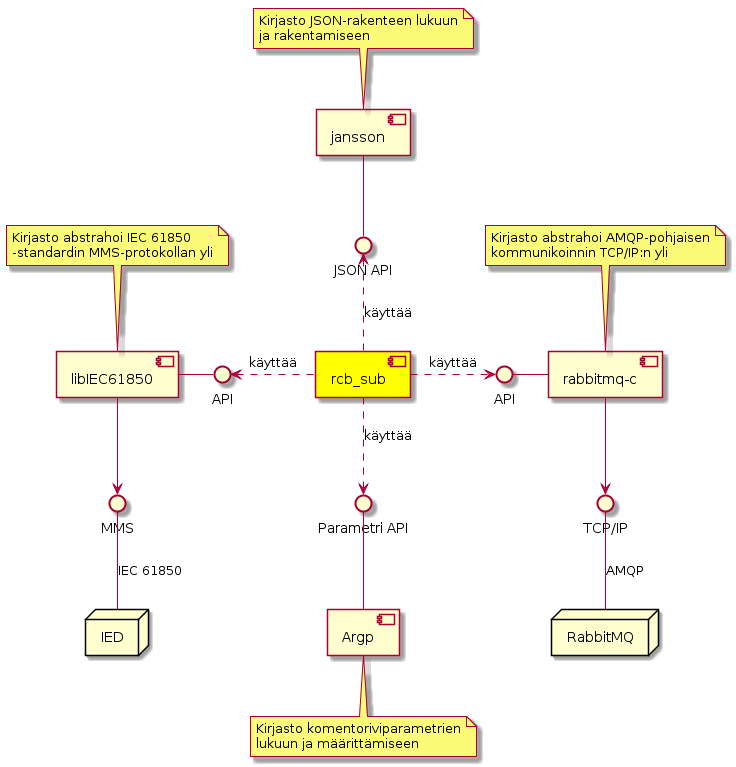
\includegraphics[width=1\textwidth]{pictures/rcb-sub-component-diagram.png}
	\caption{Toteutuksen komponenttikaavio sen osista ja relaatioista toisiinsa.}
	\label{fig:rcb-sub-komponenttikaavio}
\end{figure}

Toteutuksessa käytettiin seuraavia kirjastoja:
\begin{itemize}
	\item \emph{libiec61850},
	\item \emph{rabbitmq-c},
	\item \emph{jansson}, ja
	\item \emph{Argp}.
\end{itemize}
Kaikki käytetyt kirjastot on toteutettu C-kielellä, kuten rcb\_sub. Kirjastojen tarkoitus on abstrahoida jonkin asian käyttö, ja tarjota käyttäjälle siitä helppokäyttöinen ja ymmärrettävä rajapinta. Rajapintaa käyttämällä kirjasto hoitaa matalan tason toiminnan ilman, että sen käyttäjän tarvitsee siitä välittää. Libiec61850-kirjasto abstrahoi IEC 61850 -standardin käyttöä ja hoitaa matalan tason MMS-protokollan kommunikoinnin \mbox{\cite{libIEC61850-repo}}. Samaa kirjastoa käytettiin demoversiossa (kappale \ref{ch:demoversio-ja-sen-toiminta}) ja kirjaston kerrosarkkitehtuuri esitettiin aikaisemmin kuvassa \ref{fig:libiec61850-layer-architecture}. Kuvassa \ref{fig:rcb-sub-komponenttikaavio} libiec61850 kommunikoi suoraan IED-laitteen kanssa MMS-protokollaa käyttäen. Rabbitmq-c-kirjasto abstrahoi RabbitMQ-palvelimen käyttöä ja hoitaa matalan tason AMQP-pohjaisen kommunikoinnin \mbox{\cite{rabbitmq-c-repo}}. Toteutuksessa rabbitmq-c kommunikoi suoraan RabbitMQ-palvelimen kanssa. Jansson-kirjasto abstrahoi JSON-rakenteiden lukua ja käsittelyä C-kielelle \mbox{\cite{jansson-repo}}. Kirjastoa käytettiin rakentamaan IED-\-lait\-teel\-ta saapuneesta viestistä JSON-muotoinen viesti. JSON-rakenne on nähtävissä liitteessä \ref{ch:report-json-format}. Argp-kirjasto auttaa ohjelman komentoriviparametrien määrittämisessä ja käsittelyssä \mbox{\cite{argp-glibc-guide}}. Kirjasto auttaa toteuttamaan ohjelmalle \emph{UNIX}-tyyliset parametrit. Eli vaaditut parametrit ja vaihtoehtoiset lyhyet ja pitkä parametrit. Vaadituista parametreista esimerkiksi Linux:in komento \texttt{mv foo.txt bar.txt}, jossa \emph{foo.txt} ja \emph{bar.txt} ovat vaadittuja parametreja. Vaihtoehtoisista parametreista esimerkkinä pitkä muoto \texttt{-{}-bytes} ja lyhyt muoto \texttt{-b}. Lisäksi kirjasto lisää ohjelmaan automaattisesti Linux:ista käyttäjille tutut \texttt{-{}-help} ja \texttt{-{}-version} vaihtoehtoiset parametrit. Komennolla \texttt{-{}-help} kirjasto tulostaa Linux:ilta tutun ohjelman aputekstin käyttäjälle, jossa on esitetty ohjelman kaikki parametrit ja niiden selitteet \mbox{\cite{step-by-step-into-argp}}.

Kuvassa \ref{fig:rcb-sub-sekvenssikaavio} on esitetty rcb\_sub-ohjelman sekvenssikaavio pääpiirteisestä toiminnasta. Toteutus noudattaa suurinpiirtein samoja periaatteita kuin demo (kuva \ref{fig:sequence-diagram-report-subscription}). Tässä kohtaa käydään läpi ohjelman pääpiirteinen toiminta ja myöhemmin tarkemmin läpi kappaleessa \ref{rcb-sub-toiminta}. Ensin ohjelman suoritus alkaa lukemalla annetut parametrit Argp-kirjastolla (kohdat 1--2). Parametreissa tulee tiedot yhteyden muodostamiseen IED-laitteelle ja RabbitMQ-palvelimelle (kohdat 3--6). Parametreissa on myös tiedot RCB-instansseista jotka halutaan IED:ltä tilata. Yhteyksien muodostamisen jälkeen jokainen parametrina annettu RCB käydään läpi silmukassa ja sen arvot ja datajoukon viitteet luetaan IED:ltä (kohdat 7--12). Tämän jälkeen sisäkkäisessä silmukassa luetaan datajoukon viitteiden muuttujien \emph{spesifikaatiot} (kohdat 11--12). Spesifikaatio antaa tiedot muuttujien pituudesta ja tyypistä. Näitä tietoja käytettiin JSON-rakenteessa täydentämään viestiä (esimerkkinä liiteessä \ref{ch:report-json-format} rivit 21--22). Tämän jälkeen tehdään toinen silmukka, jossa jokainen RCB-instanssi tilataan ja niille asetetaan takaisinkutsufunktio (kohdat 13--16). Arvojen kirjoitushetkellä (kohta 15) RCB varataan ja se aloittaa viestien lähettämisen rcb\_sub-ohjelmalle. Jokaisen RCB:n kirjoituksen jälkeen ohjelma jää loputtomaan silmukkaan ottamaan viestejä vastaan (kohdat 17--22). Viestin saapuessa kutsutaan asetettua takaisinkutsufunktiota, jonka parametrina on saapunut viesti (kohta 17). Viesti muutetaan JSON-muotoon jansson-kirjastolla ja julkaistaan RabbitMQ-palvelimelle rabbitmq-c-kirjastolla (kohdat 18--21).

\begin{figure}[ht!]
	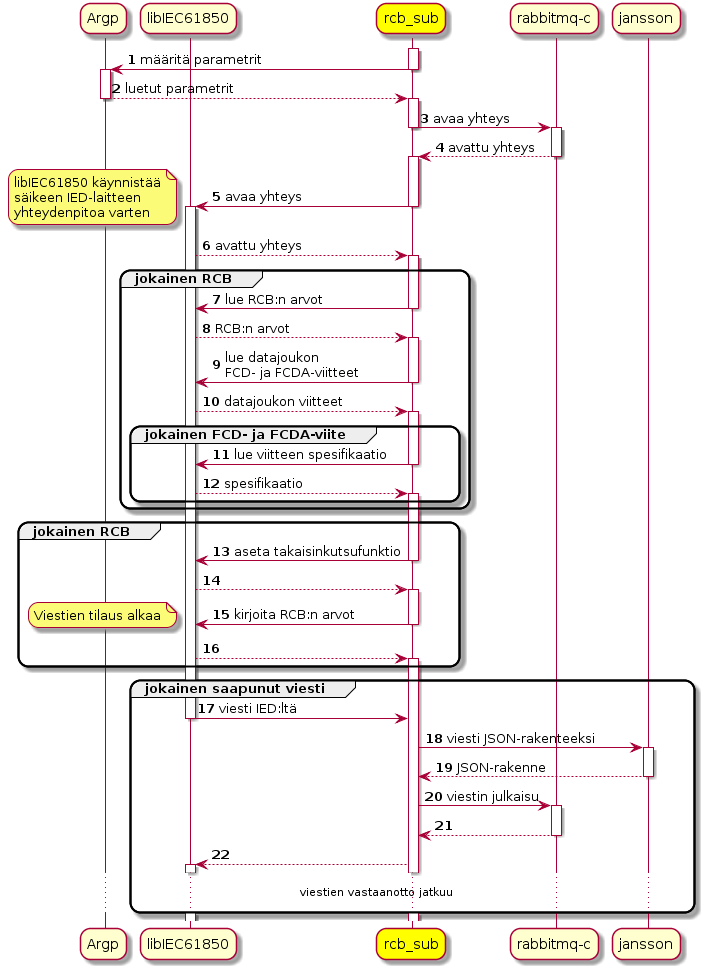
\includegraphics[width=1\textwidth]{pictures/rcb-sub-general-sd.png}
	\caption{Sekvenssikaavio rcb\_sub-ohjelman kokonaistoiminnasta.}
	\label{fig:rcb-sub-sekvenssikaavio}
\end{figure}


\section{Ohjelman toiminta}
\label{rcb-sub-toiminta}
Tulevissa kappaleissa käydään läpi yksityiskohtaisemmin rcb\_sub-ohjelman toimintaa, joka esiteltiin pääpiirteittäin kappaleessa \ref{ch:rcb-sub-yleiskuva}. Kappaleiden järjestys noudattaa kuvassa \ref{fig:rcb-sub-sekvenssikaavio} olevan sekvenssikaavion järjestystä. Toisin sanoen ohjelmaa käydään tarkemmin läpi sen suorituksen järjestyksessä.


\subsection{Parametrisointi}
Ohjelma parametrisoitiin Argp-kirjastolla. Kirjasto tarjoaa rajapinnan komentoriviparametrien käsittelyyn ja määrittämiseen. Parametrien muodot ovat tutut muista Linux-käyt\-tö\-jär\-jes\-tel\-män parametreista ja samaa periaatetta käytettiin tässäkin ohjelmassa. Kirjasto myös lisäsi ohjelmaan automaattisesti aputekstin käyttäjää varten. Aputeksti sisältää tietoa ohjelman parametreista ja niiden käytöstä. Aputekstin pystyi tulostamaan parametrilla \texttt{-{}-help}. Liitteessä \ref{ch:rcb-sub-help-output} on esitetty miltä ohjelman aputeksti näyttää. Liitteestä voi myös nähdä kaikki ohjelman parametrit ja lyhyen selityksen mihin kutakin käytetään.

Ohjelmiston parametrien voidaan ajatella koostuvan kolmesta eri ryhmästä. Ensin päätason vaihtoehtoiset parametrit \texttt{OPTIONS}. Pakolliset parametrit \texttt{EXCHANGE} ja \texttt{ROUTING\_KEY}. Viimeisenä n-kappaletta \texttt{RCB\_REF} ja \texttt{RCB\_OPTIONS} parametreja ryhmissä. Suurin osa \texttt{OPTION} parametreista on itsestäänselviä. Esimerkkinä \texttt{-{}-amqp-host}, joka kertoo A\-M\-Q\-P-pal\-ve\-li\-men IP-osoitteen, ja \texttt{-{}-ied-host}, joka kertoo IED-laitteen IP-osoitteen. Parametrit \texttt{EXCHANGE} ja \texttt{ROUTING\_KEY} määrittävät nimet RabbitMQ-palvelimen vaihteelle ja reititysavaimelle. Ryhmässä ensimmäinen \texttt{RCB\_REF} määrittää viitteen tilattavaan RCB-instanssiin IED-laitteella. Tätä seuraa vaihtoehtoinen \texttt{RCB\_OPTIONS} parametri. Se määrittää arvot, jotka kirjoitetaan edeltävä RCB-instanssille ennen tilausta. RCB-instanssin parametri \texttt{RCB\_OPTIONS} määrittää käytetyt vaihtoehtoiset kentät (\texttt{-{}-opt-fields}), käytetyt liipaisimet (\texttt{-{}-trigger}) ja pyydetäänkö yleistä kyselyä ennen muita viestejä (\texttt{-{}-gi}). Liipaisimet ja vaihtoehtoiset kentät asetetaan numeerisella arvoilla, jotka löytyvät myös aputekstistä (liite \ref{ch:rcb-sub-help-output}). Numeerisia arvoja voidaan summata yhteen, jotta voidaan asettaa monta arvoa yhtä aikaa. Liipaisimien nimet vastaavat aikaisemmin kappaleessa \ref{ch:rcb-toiminta} esitettyjä arvoja ja numeeriset arvot tulevat libIEC61850 -kirjastosta. Vaihtoehtoisten kenttien nimet vastaavat aikaisemmin taulukossa \ref{tab:iec61850-optional-fields-definition} esitettyjä arvoja ja numeeriset arvot tulevat myös libIEC61850-kirjastosta.

\subsection{Yhteyksien muodostus}
Parametrien luvun jälkeen ohjelma muodosti yhteydet ensin RabbitMQ-palvelimelle ja sen jälkeen IED-laitteelle. Kuvassa \ref{fig:rcb-sub-open-connections} on esitetty sekvenssikaavio, joka näyttä mitä kirjaston funktioita ohjelma kutsuu missäkin järjestyksessä. Funktiot ja niiden parametrit voi tarkemmin tarkistaa kirjaston omasta dokumentaatiosta. Tämä tarkentaa yleiskuvasta \ref{fig:rcb-sub-sekvenssikaavio} kohdat 3--6. Kaaviossa ohjelma muodostaa yhteydet vain kerran. Ohjelma on kuitenkin toteutettu niin, että se yrittää muodostaa yhteydet uudestaan vikatilanteissa. Jos muodostus ei onnistu, ohjelma kirjoittaa lokin tapahtuneesta ja odottaa hetken ennen uudelleen yritystä.

\begin{figure}[ht!]
	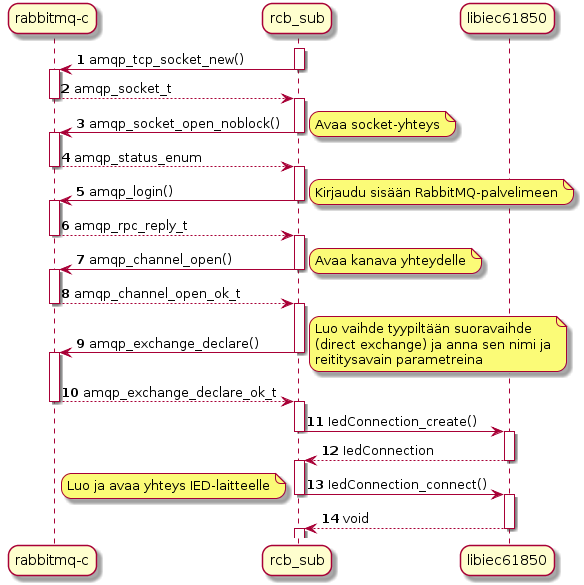
\includegraphics[width=1\textwidth]{pictures/rcb-sub-open-connections.png}
	\caption{Sekvenssikaavio kuinka rcb\_sub avaa yhteydet RabbitMQ-palvelimelle ja IED-laitteelle.}
	\label{fig:rcb-sub-open-connections}
\end{figure}

Yhteyden avauksen ja sisäänkirjautumisen jälkeen ohjelma avaa kanavan kohdassa 7--8. Kanava on yhteyden päälle avattu oma erillinen kommunikointiväylä, joka ei sotkeudu muihin kanaviin. Yhteen avattuun yhteyteen voi olla avattuna monta eri kanavaa. Kanavat mahdollistavat monen eri säikeen jakaa sama yhteys, ilman että tieto voi vuotaa toiseen säikeeseen. Kohdassa 9 kutsutaan funktiota \texttt{amqp\_exchange\_declare()}. Funktio määrittää vaihteen tyyppiä suoravaihde RabbitMQ-palvelimelle. Suoravaihde käsiteltiin kappaleessa \ref{ch:direct-exchange}. Ohjelmaan ei toteutettu parametria vaihdetyypin määrittämiseen, koska katsottiin että suoravaihde on riittävä nykyisten vaatimusten täyttämiseksi. Tulevaisuudessa voidaan tarvittaessa lisätä parametrit vaihdetyypin vaihtamiseen.


\subsection{IED:n attribuuttien tyyppin ja koon luku}
Yhteyksien muodostamisen jälkeen ohjelma käy läpi silmukassa jokaisen parametrina annetun RCB:n viitteen. Lukee RCB:n datajoukon viitteet ja selvittää jokaisen viitatun attribuutin spesifikaatiot, eli sen oikean viitteen, tyypin ja koon. Kuvassa \ref{fig:rcb-sub-reading-specifications} on esitetty sekvenssikaavio kuinka rcb\_sub tämän tekee libiec61850-kirjaston avulla. Kuva tarkentaa yleiskuvassa \ref{fig:rcb-sub-sekvenssikaavio} kohtia 7--12.

\begin{figure}[ht!]
	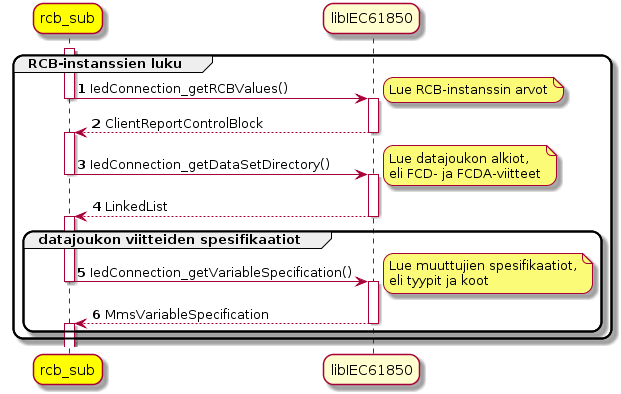
\includegraphics[width=1\textwidth]{pictures/rcb-sub-reading-specifications.png}
	\caption{Sekvenssikaavio kuinka rcb\_sub lukee RCB-instanssin arvot ja muuttujien spesifikaatiot.}
	\label{fig:rcb-sub-reading-specifications}
\end{figure}

Ensin RCB:sta luetaan sen tiedot IED-laitteelta (kohdat 1--2). RCB:ltä saadaan tieto mihin datajoukkoon se on liitetty. Tätä käsiteltiin kappaleessa \ref{ch:rcb-toiminta} ja taulukossa \ref{tab:iec61850-brcb-class-definition} kenttä \emph{DatSet}, joka kertoo käytetyn datajoukon viitteen. Tällä tiedolla ohjelma voi lukea datajoukon FCD- ja FCDA-viitteet (kohdat 3--4). Tästä saadaan jokainen viite listassa, joka käydään läpi silmukassa kohdissa 5--6. Jokaiselle viitteelle luetaan sen spesifikaatio. Spesifikaatiorakenne sisältää sisäkkäisiä spesifikaatioita, jos viite viittaa moneen muuttujaan IED-laitteen hierarkiassa. Tämä tapahtuu samalla periaatteella, jolla FCD- ja FCDA-viitteet viittaavaat moneen muuttujaan hierarkiassa alaspäin. Kuinka FCD- ja FCDA-viitteet toimivat käsiteltiin kappaleessa \ref{ch:fc-and-dataset}. Jokainen luettu viite tallennetaan ja niitä käytetään myöhemmin viestin kanssa JSON-rakenteessa. Esimerkkinä liitteessä \ref{ch:report-json-format} riveillä 21--22 tyyppi ja koko -tiedot.


\subsection{Viestien tilaus}
Ohjelman luettua kaikki muuttujien spesifikaatiot. Ohjelma tilaa silmukassa kaikki parametrina annetut RCB-instanssit. Kuvassa \ref{fig:rcb-sub-subscribe-reports} on esitetty sekvenssikaavio, kuinka rcb\_sub tilaa RCB-instanssit libiec61850-kirjaston avulla. Kuvan tarkentaa yleiskuvassa \ref{fig:rcb-sub-sekvenssikaavio} kohtia 13--16.

\begin{figure}[ht!]
	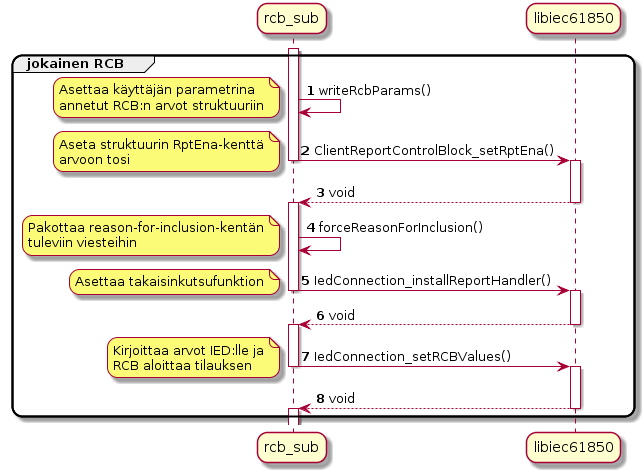
\includegraphics[width=1\textwidth]{pictures/rcb-sub-subscribe-reports.png}
	\caption{Sekvenssikaavio kuinka rcb\_sub tilaa RCB-instanssit.}
	\label{fig:rcb-sub-subscribe-reports}
\end{figure}

Ohjelma käsittelee libiec61850-kirjaston tarjoamaa \emph{ClientReportControlBlock} struktuurin instanssia. Kirjasto palauttaa struktuurin instanssin, kun RCB:n arvot luetaan IED-laitteelta. Kaikki RCB:lle kirjoitettavat arvot asetetaan instanssiin ennen IED-laitteelle kirjoitusta. Näitä arvoja ovat ohjelmalle parametreina annetut arvot, kuten liipaisimet ja vaihtoehtoiset kentät. Tämän ohjelma tekee kutsumalla omaa funktiota \texttt{wri\-teRcb\-Pa\-rams\-()} (kohta 1). Tämän jälkeen ohjelma asettaa RCB:n \emph{RptEna}-kentän arvoksi tosi (kohdat 2--3). Tämä kenttä kontrolloi RCB-instanssin varausta ja onko tilaus päällä. Seuraavaksi ohjelma pakottaa viestiin vaihtoehtoisen kentän \emph{reason-for-inclusion} (kohta 4). Tätä kenttää tarvitaan, jotta aikaisemmin luetut spesifikaatiotiedot saadaan yhdistettyä saapuneeseen viestiin. Tämän jälkeen asetetaan takaisinkutsufunktio, jota kirjasto kutsuu kun viesti saapuu (kohdat 5--6). Viimeisenä struktuurin arvot kirjoitetaan IED:llä olevalle RCB:lle (kohdat 7--8). Tämä varaa RCB-instanssin kirjoittavalle asiakkaalle, ja aloittaa tilauksen jos RptEna-kentän arvo oli tosi. RCB tulee lähettämään viestejä ohjelmalle samalla kun silmukan muilla kierroksilla käsitellään tilaamattomia RCB-instansseja.


\subsection{JSON:nin muodostaminen ja julkaisu}
Viestin saapuessa libiec61580-kirjasto kutsuu asetettua takaisinkutsufunktiota. Takaisinkutsufunktio muuttaa viestin JSON-muotoon ja lisäsi siihen aikaisemmin luetut muuttujien oikeat viittet, tyypit ja koot. Tämän jälkeen JSON-julkaistiin RabbitMQ-palvelimelle. Kuvissa \ref{fig:rcb-sub-report-to-json-1} ja \ref{fig:rcb-sub-report-to-json-2} on esitetty sekvenssikaaviolla kuinka ohjelma muuttaa viestin JSON:iksi ja julkaisee RabbitMQ:lle. Kuva \ref{fig:rcb-sub-report-to-json-1} jatkuu kuvassa \ref{fig:rcb-sub-report-to-json-2}. Kuva \ref{fig:rcb-sub-report-to-json-1} tarkentaa yleiskuvan \ref{fig:rcb-sub-sekvenssikaavio} kohtia 17--19 ja kuva \ref{fig:rcb-sub-report-to-json-2} kohtia 20--22.

\begin{figure}[ht!]
	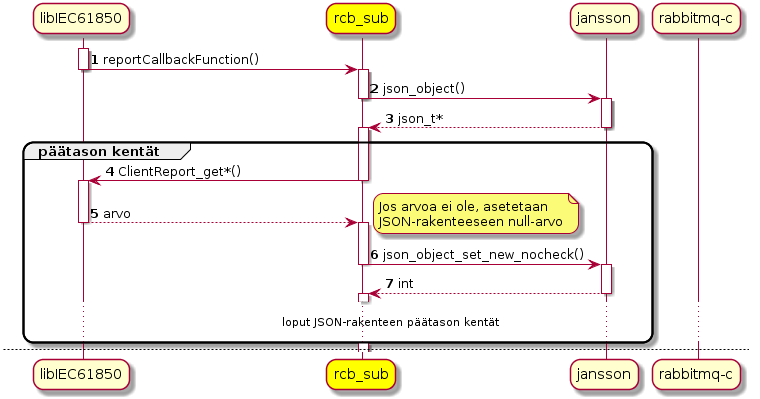
\includegraphics[width=1\textwidth]{pictures/rcb-sub-report-to-json.png}
	\caption{Sekvenssikaavio kuinka rcb\_sub muodostaa JSON:nin päätason kentät.}
	\label{fig:rcb-sub-report-to-json-1}
\end{figure}

Kuvassa \ref{fig:rcb-sub-report-to-json-1} suoritus alkaa kun libiec61850-kirjasto kutsuu takaisinkutsufunktiota. Funktiolle annetaan parametrina saapunut viesti \emph{ClientReport}-struktuurin instanssina (kohta 1). Tämän jälkeen ohjelma käy läpi viestin jokaisen päätason kentän ja lisää ne JSON-rakenteeseen. Osa viestin kentistä on vaihtoehtoisia riippuen siitä, mitä käyttäjä asetti \texttt{-{}-opt\--\-fields} parametrilla. Jos arvoa viestissä ei ole, korvataan se null-arvolla JSON:iin. Esimerkkinä liiteessä \ref{ch:report-json-format} rivillä 4 oleva \texttt{confRevision} muuttuja, jonka arvo on null. Tämän jälkeen suoritus jatkuu kuvasta \ref{fig:rcb-sub-report-to-json-1} kuvaan \ref{fig:rcb-sub-report-to-json-2}.

\begin{figure}[ht!]
	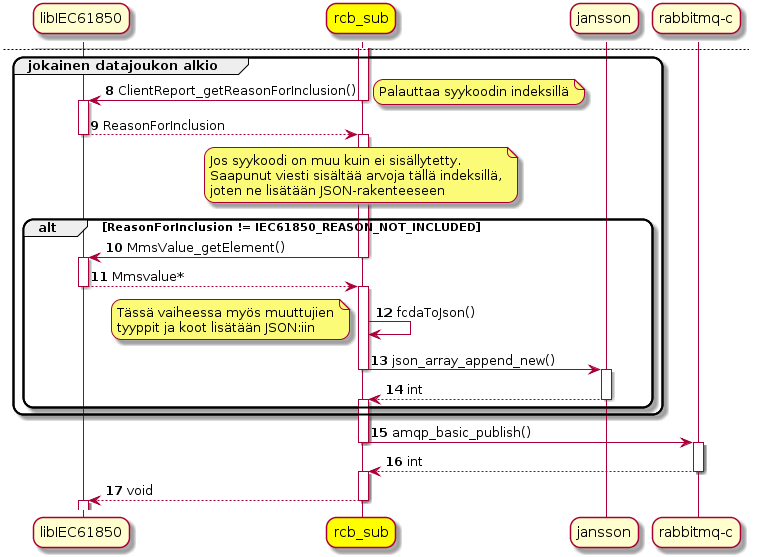
\includegraphics[width=1\textwidth]{pictures/rcb-sub-report-to-json_001.png}
	\caption{Sekvenssikaavio kuinka rcb\_sub lisää JSON:iin muuttujat viestistä.}
	\label{fig:rcb-sub-report-to-json-2}
\end{figure}

Päätason viestin kenttien jälkeen ohjelma käy läpi silmukassa viestin datajoukon indeksit (kuvassa \ref{fig:rcb-sub-report-to-json-2} kohdat 8--14). Viesti oikeasti sisältää vain ne datajoukon alkiot, jotka sisältyivät viestiin. Ongelmana tässä on se, että viesti ei sisällä indeksiä tai tietoa siitä mikä datajoukon alkio on kyseessä. Jotta tästä saadaan tieto, ohjelma pakottaa syykoodin päälle viestiin. Tämän avulla kun silmukassa käydään kaikki datajoukon indeksit läpi, voidaan jokaiselle indeksille ensin kysyä syykoodi viestistä (kohdat 8--9). Jos datajoukon alkio ei ole viestissä, palauttaa kirjaston funktio \texttt{Cli\-entRe\-port\-\_\-get\-Rea\-son\-For\-Inc\-lu\-si\-on\-()} arvon \texttt{IEC61850\_REASON\_NOT\_INCLUDED}. Tätä tietoa voidaan käyttää löytämään oikea datajoukon indeksi. Jos datajoukon indeksi on viestissä, suoritetaan kohdat 10--14, muuten mennään seuraavaan indeksiin ja toistetaan kohdat 8--9. Datajoukon indeksi tarvitaan, jotta aiemmin luetut spesifikaatiot saadaan yhdistettyä attribuutteihin arvojen kanssa. Datajoukon indeksillä, viestin arvoilla ja muuttujien tyypeillä ja koolla saadaan rakennettua loppuosa JSON-rakenteesta. Kuvassa \ref{fig:rcb-sub-report-to-json-2} oleva silmukka rakentaa liitteessä \ref{ch:report-json-format} olevan values-taulun alkaen riviltä 7. JSON:in sisempi values-taulu (rivi 13) on lista FCD- tai FCDA-viitteen muuttujia, mitä se viittaa arvoineen. Tämä taulukko muodostetaan kuvan \ref{fig:rcb-sub-report-to-json-2} kohdassa 12 funktiolla \texttt{fcdaToJson()} ja lisätään JSON:iin kohdassa 13. Lopuksi viesti lähetetään RabbitMQ-palvelimelle funktiolla \texttt{amqp\_basic\_publish()} ja takaisinkutsufunktio palaa (kohdat 15--17).

\section{Jatkokehitys}
Ohjelma jätettiin työssä pisteeseen, missä se saavutti kaikki sille asetetut vaatimukset. Kuitenkin tulevaisuudessa ohjelmaa voidaan lisätä ominaisuuksia tarpeen vaatiessa. Isoin puute ohjelmassa oli testiympäristö ja sen yksikkötestit. C:ssä ei ole suoraan tukea yksikkötestien kirjoittamiseen. Ympäristön pystytys vaatii erillisen kirjaston projektin yhteyteen, millä yksikkötestit kirjoitetaan. Tämä jäi tulevaisuuden kehitystyöksi ja ei sisältynyt tähän työhön. Yksikkötestit ovat kuitenkin tärkeä osa ohjelman ylläpitoa ja toiminnan varmistamista muutosten jälkeen. Testit tullaan tarvitsemaan ennemmin tai myöhemmin.

Ohjelma toteutettiin nyt niin, että se aina käyttää suoraa vaihdetyyppiä RabbitMQ-pal\-ve\-li\-mel\-la. Tämä täytti työlle asetetut vaatimukset. Jos tulevaisuudessa tarvitaan joustavuutta, voidaan ohjelmaan tehdä muutoksia ja parametreja lisätä helposti lisämään toiminnallisuutta. Esimerkkinä käyttäjä voisi valita käytettävän vaihteen tyypin parametrilla.
\chapter{Arviointi}
\label{ch:arviointi}
Kirjoitta tähän arviota työn tuloksista. Peilataanko tässä kysymyksiä vai tuloksissa? Mikä tämän kappaleen ero on tuloksiin nähden?
\chapter{Tulokset}
\label{ch:tulokset}
\begin{it}
	Kirjoita tähän lopputuloksen analysoinnista ja peilaa saatuja tuloksia työlle alussa asetettuihin kysymyksiin. Mitä jäi saavuttamatta, mitä saavutettiin ja miten hyvin? Mitä olisi voinut parantaa? Voi jakaa aliotsikoihin jos tarvetta.
\end{it}
\chapter{Yhteenveto}
\label{ch:yhteenveto}
% Diplomityön tuloksena saatiin ohjelmistokomponentti osaksi muuta sähköasemiin liittyvää järjestelmää.
Diplomityön tuloksena saatiin ohjelmistokomponentti osaksi isompaa sähköasemiin liittyvää järjestelmää. Komponentti kykeni tilaamaan viestejä IED-laitteelta IEC 61850 -stan\-dar\-din mukaisesti, muuntamaan viestit JSON-muotoon ja jakamaan sen muun järjestelmän kanssa. Viestien jako järjestelmässä toteutettiin AMQP-standardiin pohjautuvalla välittäjäpalvelimella, joka käyttää julkaisija-tilaaja- ja viestijono-kom\-mu\-ni\-koin\-ti\-pa\-ra\-dig\-mo\-ja. Toteutetun systeemin arkkitehtuuri esitettiin kuvassa \ref{fig:planned-system-architecture}. Arkkitehtuurissa muu järjestelmä on vastuussa tilauksien orkestroinnissa ja rcb\_sub-prosessien suorituksesta.

% Yhteenveto asetetuista vaatimuksista ja kuinka ne saavutettiin.
Diplomityön alussa asetettiin vaatimuksia jotka toteutuksen pitäisi pystyä täyttämään. Taulukossa \ref{tab:requirements-met} on esitetty yhteenveto asetetuista vaatimuksista ja kuinka ne tuontantoversiossa on täytetty. Taulukossa vaatimukset on esitetty niiden tunnuksilla, jotka asetettiin aikaisemmin kappaleessa \ref{ch:vaatimukset}.

\begin{table}[ht!]
	\caption{Yhteenveto asetetuista vaatimuksiin ja kuinka ne täytettiin.}
	\label{tab:requirements-met}
	\begin{tabular}{p{0.11\linewidth} | p{0.82\linewidth}}
		\hline
		\textbf{Vaatimus\-tunnus} & \textbf{Kuinka vaatimus täytettiin} \\
		\hline
		% viestien tilaus sähköasemalta IEC 61850 -standardin mukaisesti
		V1 & Viestit tilattiin käyttämällä libIEC61850-kirjastoa, joka hoitaa standardin mukaisen matalan tason kommunikoinnin. \\
		\hline
		% tilattujen viestien jakaminen järjestelmässä siitä kiinnostuvien komponenttien kanssa
		V2 & Viestien jakamiseen käytettiin viestijono- ja julkaisija-tilaaja-kommunikointiparadigmoja, jotka toteutettiin AMQP-standarin mukaisella RabbitMQ-välittäjäohjelmistolla. \\
		\hline
		% tilattuja viestejä haluavien komponenttien määrä pitää pystyä muuttumaan järjestelmän tarpeiden mukaan
		V3 & Komponentit pystyvät tilaamaan viestejä RabbitMQ-välittäjältä julkaisija-tilaaja-paradigman mukaan. Tilaajien määrää ei ole rajoitettu. \\
		\hline
		% muu järjestelmä ohjaa milloin viestien tilaus sähköasemilta aloitetaan ja lopetetaan
		V4 & Järjestelmä ajaa rcb\_sub-ohjelmaa taustaprosessina ja antaa tilauksen tarvittavat tiedot sille komentoriviparametreillä. \\
		\hline
		% komponenttien täytyy saada ilmoitus uudesta viestistä ilman erillistä kyselyä
		V5 & RabbitMQ-välittäjä tarjoaa ilmoituksen tilaajalle kun uusi viesti julkaistaan. \\
		\hline
		% viestit puskuroidaan myöhempää käsittelyä varten jos komponentti ei ehdi niitä heti käsitellä
		V6 & RabbitMQ-välittäjä tarjoaa viestijonoparadigman mukaisen jonon, jos tilaaja ei ehdi viestiä käsitellä. \\
		\hline
		% komponentin pitää pystyä suodattamaan viestit sen lähteen identiteetin perusteella
		V7 & Rcb\_sub julkaisee viestit RabbitMQ-välittäjälle IED-laitteen tunnisteella, jolloin tilaaja voi tilata haluamansa viestit. \\
		\hline
		% viestien jakamisen muoto pitää olla helposti ymmärrettävä järjestelmän osapuolien kesken
		V8 & IEC 61850 -standardin mukainen binääritason viesti muutettiin JSON-muotoon, joka on helpommin luettavissa ohjelmistolle ja ihmiselle. \\
		\hline
		% sähköasemalta tilattavien viestien määrä pitää pystyä muuttumaan tilauksien välillä
		V9 & Rcb\_sub-ohjelmaa ajetaan taustaprosessina ja järjestelmä voi muuttaa tilauksen tietoja (RCB-instassien määrä) syöttämällä eri komentoriviparametrit käynnistyksen yhteydessä. \\
		\hline
		% viestien välitystekniikka järjestelmässä täytyy tukea verkkopalvelun tapauksessa TCP/IP-protokollamäärityksiä
		V10 & MMS-protokolla ja valittu AMQP-standardi toimivat TCP/IP-protokollaperheen päällä. \\
		\hline
		% tiedonsiirrossa lähetystakuu ei ole välttämättömyys
		V11 & AMQP tarjoaa lähetystakuumekanismit julkaisijoiden ja tilaajien välille. \\
		\hline
	\end{tabular}
\end{table}

% Lähtökohtien avulla huomattiin että järjestelmän kommunikointiin tarvittiin viestijonoparadigma ja joukkokommunikointi tai julkaisija-tilaaja.
Työssä ratkaisua lähdettiin etsimään tarkastelemalla ensin hajautetun järjestelmän teoriaa, sen kommunikointiparadigmoja ja IEC 61850 -standardin määrityksiä. Saatuja tietoja apuna käyttäen suunniteltiin arkkitehtuuri osaksi muuta järjestelmää. Huomattiin, että viestijonoparadigma tarvittiin viestien puskurointiin ja kommunikointiin sopi jouk\-ko\-kom\-mu\-ni\-koin\-ti- tai julkaisija-tilaaja-paradigma.

% Toteutuksen tekniikaksi valittiin AMQP-standardi ja viesti päädyttiin muuntamaan JSON-muotoon.
Järjestelmän kommunikointiin valittiin AMQP-standardi, jonka myötä julkaisija-tilaaja-paradigma päätyi toteutukseen joukkokommunikoinnin sijaan. AMQP ei suoraan ollut tarkoitettu joukkokommunikoinnin toteuttamiseen. IEC 61850 -standardi määritti, että viestit IED-laitteelta tilataan julkaisija-tilaaja-paradigman mukaan. Toteutetun ohjelmiston ja valittujen paradigmojen voidaan sanoa jatkavan IED-laitteen tilausmekanismia ja näin ollen sopivat toteutukseen. Toteutus sallii monen tilaajan tilata sama viesti, mitä IEC 61850 -standardi ei ilman erillistä RCB-instanssia mahdollistanut. Viestin sisältö päädyttiin muuttamaan JSON-muotoon helpomman luettavuuden takia verrattuna MMS-protokollan binääriseen esitysmuotoon. Ohjelman tekemä JSON-muoto on nähtävissä liitteessä \ref{ch:report-json-format}. Edellä mainittujen pohjalta näiden osalta asetettuihin vaatimuksiin päästiin hyvin ja ne saatiin täytettyä. Nämä myös antavat vastaukset tutkimuskysymyksiin T1, T2 ja T3.

% Demon ongelmat ja niiden syyt.
Ennen diplomityön aloitusta tekijä oli yrityksessä toteuttanut demon ohjelmiston toimivuudesta. Demo oli tie oppia IEC 61850 -standardin toimintaa ja perehtyä aiheeseen tarkemmin ennen oikeaa toteutusta. Demossa oli kuitenkin ongelmia, mitkä haittasivat sen jatkokehitystä. Diplomityössä analysoitiin demon ongelmia, joita olivat huono suorituskyky, muistivuoto ja toiminnan epävarmuus. Toiminnan epävarmuuteen ja huonoon suorituskykyyn oli syynä Ruby-kielen oletustulkissa oleva globaali tulkkilukitus (GIL/GVL). Ja muistivuoto aiheutui huonosta Ruby-koodin ja C-kielen integraatiosta.

% Kuinka tekniset ongelmat ratkottiin toteutetussa ohjelmistossa.
Toteutetun ohjelman suorituskykyä saatiin paremmaksi valitsemalla matalamman tason C-ohjelmointikieli. C on käännettävä kieli verrattuna Ruby:n tulkattavaan kieleen. Lisäksi C voi hyödyntää käyttöjärjestelmän säikeitä ilman rajoituksia verrattuna Ruby-tulkin globaaliin lukitukseen. Muistivuoto saatiin korjattua huolellisella ohjelmoinnilla ja varmistamalla, että muisti vapautettiin, kun sitä ei enää tarvittu. Kielen valinnalla ohjelman muistinkäyttö saatiin entiseen nähden pienemmäksi. Ruby:llä toteutettu demo käytti muistia noin 150 Mt ja rcb\_sub käytti noin 4 kt. Toteutetussa ohjelmassa ei ollut demossa havaittavia ongelmia ja on osoittautunut tuotannossa toimivaksi muun järjestelmän kanssa. Edellä mainittujen perusteella demon analyysi onnistui ja sen pohjalta toteutukseen tehtiin oikeita teknisiä valintoja. Tämä myös vastaa tukimuskysymykseen T4.

% Toteutettu ohjelma on toiminut hyvin ja päästiin asetettuihin tavoitteisiin.
Toteutettu ohjelmisto on tuotannossa osana muuta järjestelmä ja diplomityön kirjoittamisen valmiiksi saamiseen asti on toiminut ongelmitta. Kappaleessa \ref{ch:arviointi} arvioitiin ja pohdittiin saatuja tuloksia. Näiden pohjalta voidaan sanoa, että diplomityössä suunniteltu toteutus pääsi asetettuihin tavoitteisiin ja tutkimuskysymyksiin löydettiin vastaus. Toteutus ei kuitenkaan ole täydellinen ja siinä on parannettavaa. Näihin kohtiin tullaan yrityksessä palaamaan tulevaisuudessa ja muuttamaan niitä, mikäli tarve vaatii. Tämän diplomityön tulokset tarjoavat myös apua samankaltaisten järjestelmien suunnitteluun ja toteutukseen.


% This can be deleted later.
\begin{it}
	Kommentteja työtä aloittaessa:
	\begin{itemize}
		\item Olisiko hyvä, että lähdet työssäsi erilaisista hajautus paradigmoista (push vs pull; message queue), perustelet valintasi ja sitten menet suunnitteluun ja toteutukseen?
		\item Ja olisi hyvä, että työ perustelee miksi tuota MQ arkkitehtuuria yleensä (ja rabbitMQ:ta) käytetään.
	\end{itemize}
	
	Things to do now:
	\begin{itemize}
		\item Laittaa aihe hyväksyntään.
		\item Lähde kirjoittamaan teoriaa ja ennen sitä yleistä tasoa missä ollaan. Yleinen korkea taso sen takia, että lukija ymmärtää mistä edes on kyse. Pidä koko ajan kirjoittaessa mielessä top-down lähestymistapa! Erittäin tärkeä!!!
		\item Loppu otsikoida niin että ensin on tulokset, niiden arviointi ja yhteenveto mainitussa järjestyksessä.
		\item Kirjoittaessa miettiä asioita mistä kirjoitetaan ja pitää kontekstista kiinni.
		\item Pidä lauseet simppelineinä ja helppolukuisina! Älä turhaan vaikeuta hommaa lukijalle ja se ei tuo työhön yhtään mitään lisäarvoa! Todella tärkeä asia ajatella! Jos lause käsittää monta asiaa, pilko se pienempiin erillisiin lauseisiin.
		\item Muihinkin lähteisiin voi viitata kuin tieteellisiin. Toki yritä löytää tieteellisiä julkaisuja mahdollisuuksien mukaan. Osoittaa että olet perehtynyt asiaan paremmin.
		\item Kun kirjoitat asiaa esim. että entisessä ohjelmassa oli ongelma että ei skaalaudu helposti tai on huono suorityskyky. Kerro mistä johtopäätös tulee. Tämä ei ole lukijalle selvää tietoa.
		\item Teorien ja yleisen osuuden kirjoittamisen jälkeen, sovi palaveri Karin kanssa.
		\item Työn otsikko on hyvä, ei tarvitse olla erikseen "ohjelmallisesti" sanaa.
		\item Työn päätason otsikoita laittaa enemmän kuvaavimmiksi kuin "Alkutilanne" ja "Teoria".
		\item Käytä työssä viesti sanaa raportin sijaan. Tuo lukijalle esille että se tarkoittaa standardin mukaisia raportteja.
	\end{itemize}
	
	Huomioituja asioita toisten dipoissa:
	\begin{itemize}
		\item Tärkeät sanat esitellään tekstissä ensimmäisen kerran kursiivilla painottamisen takia. Tämän jälkeen ei enää samaa sanaa kursivoida.
		\item Todella paljon erilaisia lähteitä käytetty! Blogiposteja, kirjoja, ja tapahtumien kirjoituksia (IEEE). On myös nettisivuja käytetty lähteenä kun mainitaan esim. Git ja jotain muita sivuja. Nämä tietysti voi olla myös alaliitteenä sivulla.
		\item Tosi hyvin kirjoitettu! Todella selkeää tekstiä ja etenee hyvin ja on lukijalle ystävällinen.
		\item Johdanto on pilkottu otsikoihin työn alkutilanteen selvittämiseksi hyvin ennen teoriaa. Ja teoriaosuus alkaa joustavasti johdannon jälkeen järkevästi.
		\item Kun listataan tekstiä, sana on ensin \emph{kursiivilla} ja on selitetty asiaa. Kohta loppuu puolipisteeseen (;). Tämän jälkeen jatkuu pienellä seuraava aihe ja päättyy myös puolipisteeseen. Viimeinen kohta alkaa myös pienellä, mutta päättyy pisteeseen normaalisti. Seuraava kappale alkaa normaalisti. Listassa lauseet muokkautuvat yhteen esim. käyttäen ja sanaa.
		\item Kysymys teoriassa mikä työssä on jäljellä oli kirjoitettu \emph{kursiivilla}.
	\end{itemize}
\end{it}


% This adds used sources chapter.
\addto\extrasenglish{\btxifchangecaseoff} % Controls the case-changing for English titles. Make sure that case is preserved for abbreviations and proper nouns, e.g. title={The {ABC} of {Tex}: An Introduction to the Typesetting System}

\ifnameyear
  \bibliographystyle{babapaliktutnat}
\else
  \bibliographystyle{bababbrtut}
\fi
\bibliography{references}


% Starts the appendix part.
\appendix

% Appendix chapters here.
%\chapter{Testiliite}
%\label{ch:classdocumentation}


\end{document}